\documentclass[a4paper,12pt]{article}
\usepackage[utf8]{inputenc}
\usepackage{graphicx}
\usepackage{amsmath}
\usepackage{hyperref}
\usepackage{longtable}
\usepackage{fancyhdr}
\usepackage{float}
\usepackage{geometry}
\geometry{margin=1in}
\usepackage{natbib}





\begin{document}
% Title Page
\begin{titlepage}
    \begin{center}
        % University Logo
        
\includegraphics[width=0.8\textwidth]{graphs/uni_logo.png} \\[1.5cm]  
        
        
        \textbf{\Large CMP5352 Data Visualization} \\[0.5cm]
        \textbf{\large Dry Bean Dataset Visualization} \\[0.5cm]
        
       
        \textbf{Prepared by: Solomon Silwal} \\[0.5cm]
        \textbf{Student Id: 23189650} \\[0.5cm]
    \end{center}
\end{titlepage}

\tableofcontents
\listoffigures


\newpage

\section{Introduction}
The Dry Bean Dataset used in this analysis comes from the UCI Machine Learning Repository. It includes several physical measurements of seven different types of beans: BARBUNYA, BOMBAY, CALI, DERMASON, HOROZ, SEKER, and SIRA. This report aims to explore and visualize the dataset to better understand the relationships between the features, using various visualization techniques \cite{chawathe2021classification}. The insights obtained can help improve our understanding of the characteristics that differentiate these bean types, which can further be applied to practical classification problems in agriculture.

\subsection{Background}
The dataset contains detailed geometric features such as Area, Perimeter, Major Axis Length, Minor Axis Length, Compactness, Eccentricity, Solidity, and several shape factors. These measurements allow for the study of bean morphology and their distinguishing characteristics \cite{pena2021morphometry}.Understanding these features is critical for identifying variations among different bean types, which can ultimately aid in developing more efficient classification models.

\subsection{Dataset Description}
The dataset contains 13 features and 7 classes of beans, with over 13,000 records. The large number of records ensures a comprehensive analysis of the bean types, providing ample data to identify meaningful patterns and trends. The main objective of this analysis is to explore the dataset in detail and identify patterns among different classes using a variety of statistical and visualization methods. Such exploration will provide valuable insights that can be used in machine learning models for accurate classification.

\subsection{Data Features}
The dataset includes numeric features such as Area, Perimeter, Compactness, Eccentricity, Shape Factors, and more. These features help in classifying different bean types by capturing various aspects of their geometry. For example, Area and Perimeter provide information on the size, while Compactness and Eccentricity describe the shape and form of the beans. Analyzing these features in depth allows us to determine which attributes are most significant in distinguishing between bean classes.

\subsection{Purpose of Study}
The aim of this report is to analyze the dataset and gain insight into which features best differentiate between the bean classes. This knowledge is useful for building models for classification or clustering purposes. By understanding the relationships between features and their impact on classification, we can develop more effective predictive models. Additionally, these insights can contribute to improvements in agricultural practices, such as automated sorting and quality control of dry beans, ultimately enhancing efficiency and reducing manual labor.


\newpage
\section{Literature Review}

The use of data visualization and machine learning is critical in agricultural data analysis, especially for classification and quality control tasks.

\subsection{Data Visualization Techniques}
Data visualization techniques like scatter plots and heatmaps aid in understanding feature relationships and identifying patterns. \citet{chawathe2021classification} highlighted how visualizations can uncover trends in agricultural datasets. Similarly, \citet{pena2021morphometry} noted the role of visualization in detecting outliers and distribution patterns.

\subsection{Machine Learning for Agricultural Classification}
Feature selection is vital for enhancing model performance. \citet{gautam2022feature} emphasized the benefits of dimensionality reduction methods like PCA for classification accuracy improvement. Various machine learning techniques, including decision trees and ensemble methods, have shown effectiveness in agricultural classification tasks.

\subsection{Agricultural Automation and Quality Control}
Automation significantly reduces manual labor while ensuring consistent quality in agriculture. \citet{sandeep2022modern} discussed the impact of automation on sorting and grading, although challenges remain due to variability in product characteristics.

\subsection{Challenges and Future Directions}
Challenges include handling data variability and noise. Future directions suggest using deep learning techniques like convolutional neural networks and adopting methods such as model ensembling and hyperparameter tuning for robust model performance \cite{khan2023comparison}.



\newpage

\section{Motivation and Objectives}
The motivation behind this work is to explore agricultural datasets and gain insights into the morphometric features of dry beans, which are crucial in agriculture and food industries. By analyzing these features, we aim to contribute towards automation in quality control, improving classification models, and advancing agricultural practices. Efficient sorting and classification of agricultural products are essential to enhance productivity and reduce manual labor, making this study highly relevant.

Understanding the characteristics of different bean types also aids in optimizing processes from harvest to market, ensuring quality standards. This motivates our exploration of data to identify key attributes that differentiate between bean classes, ultimately improving decision-making in the agricultural sector.

The objectives of this study are as follows:
\begin{itemize}
    \item \textbf{To explore and visualize the Dry Bean Dataset}: Conduct an in-depth exploration of the dataset to uncover trends, patterns, and outliers, enhancing our understanding of the data.
    
    \item \textbf{To identify correlations and patterns between features}: Analyze relationships between features to understand their structure and determine which attributes are most important for classification.
    
    \item \textbf{To generate insights for machine learning models}: Use the findings to support the development of machine learning models for bean classification, focusing on effective feature selection and engineering \cite{gautam2022feature}.
    
    \item \textbf{To contribute to agricultural automation}: Apply insights to automate sorting and grading processes, reducing manual labor while ensuring consistent quality.
\end{itemize}

Overall, this study aims to apply data-driven techniques to improve classification, automation, and quality control in the agricultural sector, with a specific focus on dry beans.

\section{Methodology}
The methodology adopted in this report consists of data preprocessing, exploration, visualization, and analysis. The major steps include:
\begin{enumerate}
    \item Loading and cleaning the dataset.
    \item Checking for missing and duplicate values.
    \item Exploring relationships between features using visualizations such as density plots, box plots, scatter plots, and heatmaps.
    \item Using interactive visualizations to aid in a more in-depth understanding of the dataset.
\end{enumerate}

\newpage

\section{Data Exploration}
\subsection{Dataset Overview}
The dataset consists of 13 features describing the morphometric properties of different bean types. Each feature provides information that can help distinguish one type from another.

\subsection{Handling Missing Values}
During the exploration process, no missing values were found in the dataset. A summary of the dataset was created to check the distribution of each variable.

\begin{figure}[H]
    \centering
    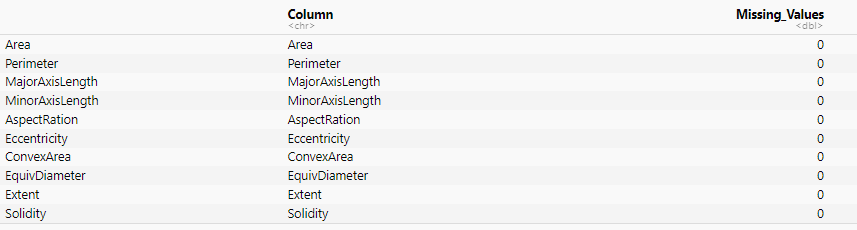
\includegraphics[width=0.8\textwidth]{graphs/missing1.png}
    \caption{Summary of Missing Values - Part 1}
    \label{fig:missing_values_1}
\end{figure}

\begin{figure}[H]
    \centering
    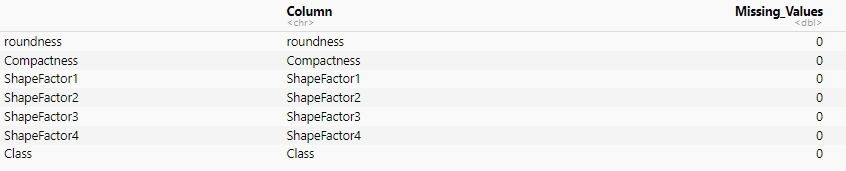
\includegraphics[width=0.8\textwidth]{graphs/missing2.png}
    \caption{Summary of Missing Values - Part 2}
    \label{fig:missing_values_2}
\end{figure}

\subsection{Duplicate Values}
Duplicate values were identified and removed, as they could affect the analysis. The dataset initially contained a small percentage of duplicates, which were dropped before proceeding with the analysis.

\begin{figure}[H]
    \centering
    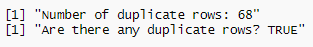
\includegraphics[width=0.5\textwidth]{graphs/duplicate.png}
    \caption{Summary of Duplicate Values}
    \label{fig:duplicate_values}
\end{figure}

\newpage

\section{Data Visualization}
To gain a comprehensive understanding of the dataset, several visualizations were created.An interactive Shiny app dashboard has also been developed to explore these visualizations in a more dynamic way. You can access the dashboard here: \url{https://solomonsilwal.shinyapps.io/Dry_Bean_Visualization_SolomonSilwal/}.


\subsection{Distribution Plot of Bean Classes}
\noindent\textbf{Objective:} This plot helps to understand the distribution of the different bean classes in the dataset. It answers the question: "How are the various bean types represented in the data?"

\noindent\textbf{Explanation:} By examining the number of instances for each class, the plot highlights any class imbalances that could impact the accuracy of classification models. Understanding class distribution helps to anticipate potential challenges in model training.
\begin{figure}[H]
    \centering
    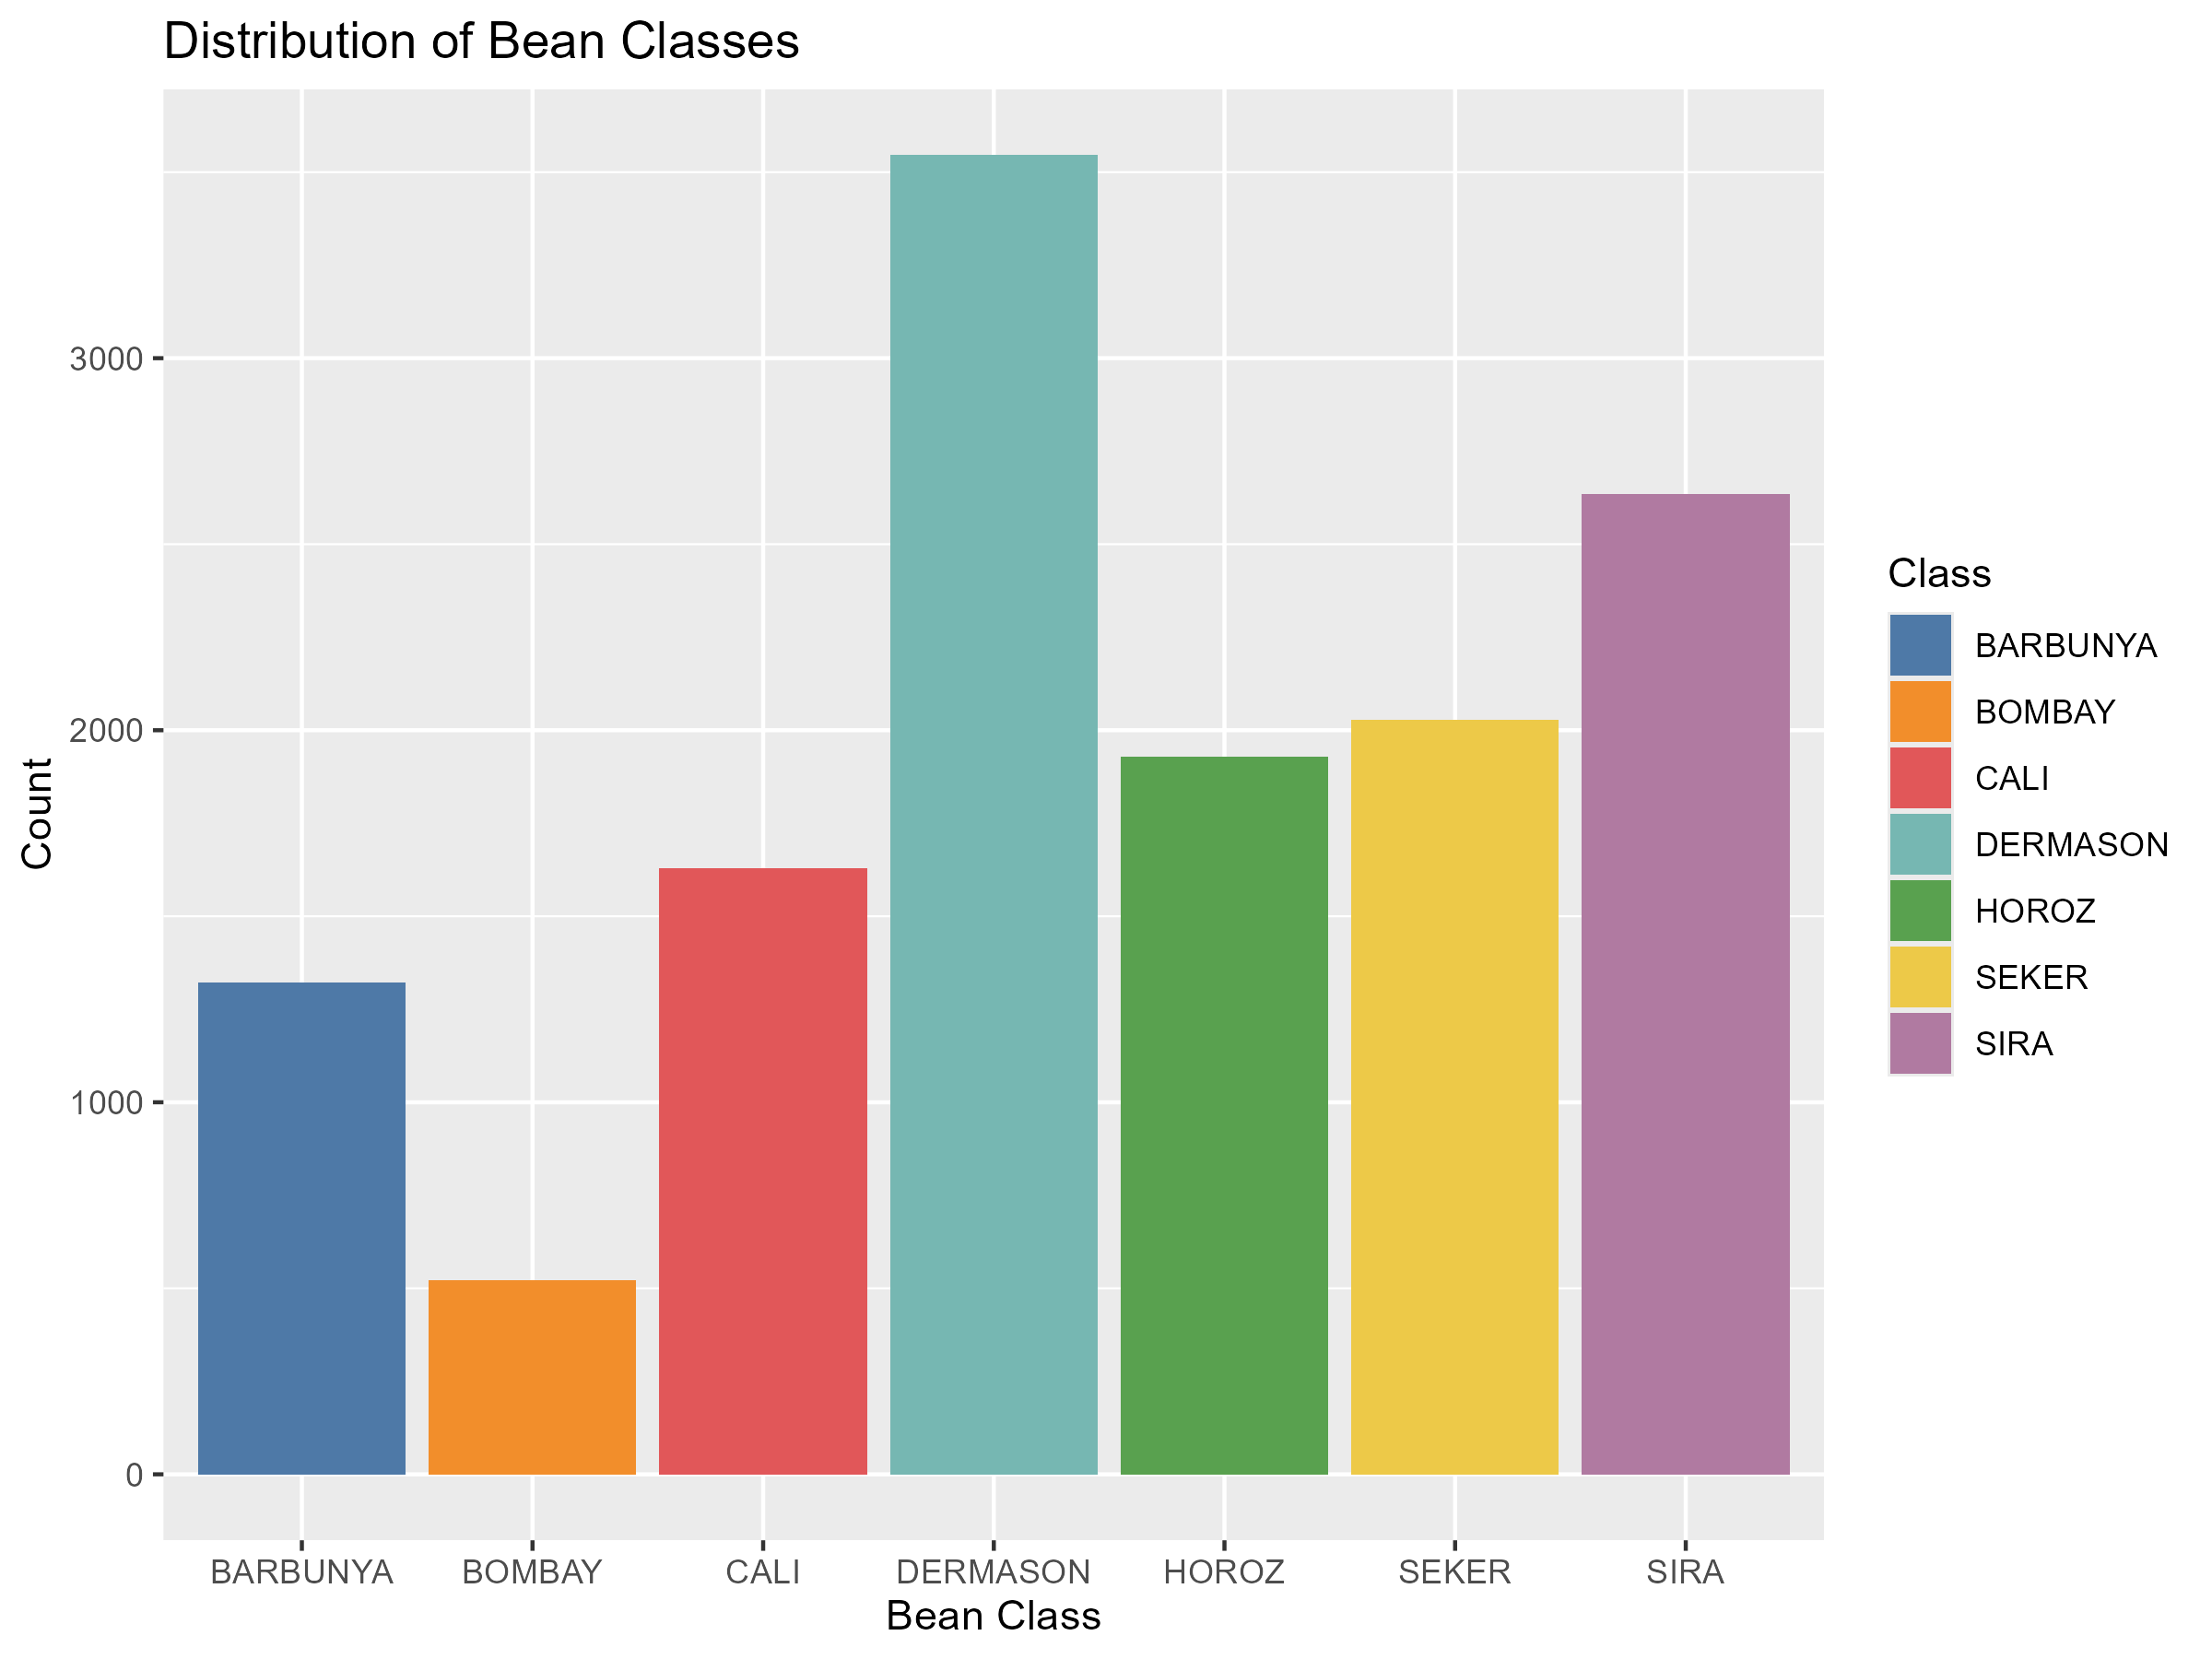
\includegraphics[width=0.8\textwidth]{graphs/bean_class_distribution.png}
    \caption{Distribution of Bean Classes}
    \label{fig:distribution_classes}
\end{figure}
The bar plot above shows the distribution of different bean classes. The x-axis represents the seven distinct bean classes, while the y-axis shows the count of instances for each class. The DERMASON class has the highest count, followed by SIRA, CALI, and HOROZ. BOMBAY has the lowest count. Understanding class distribution helps analyze the representation of each class in the dataset and informs classification model training by highlighting potential imbalances.

\newpage

\subsection{Density Plot of Area by Bean Class}
\noindent\textbf{Objective:} This visualization explores the variation in the \textit{Area} attribute across different bean classes. It addresses the question: "What are the typical ranges of the \textit{Area} attribute for each bean class?"

\noindent\textbf{Explanation:} The density plot shows that most bean classes, such as BARBUNYA and SIRA, have \textit{Area} values concentrated between 40,000 and 60,000. BOMBAY beans, however, exhibit a wider range, with values extending beyond 100,000, indicating more variability in size.

\begin{figure}[H]
    \centering
    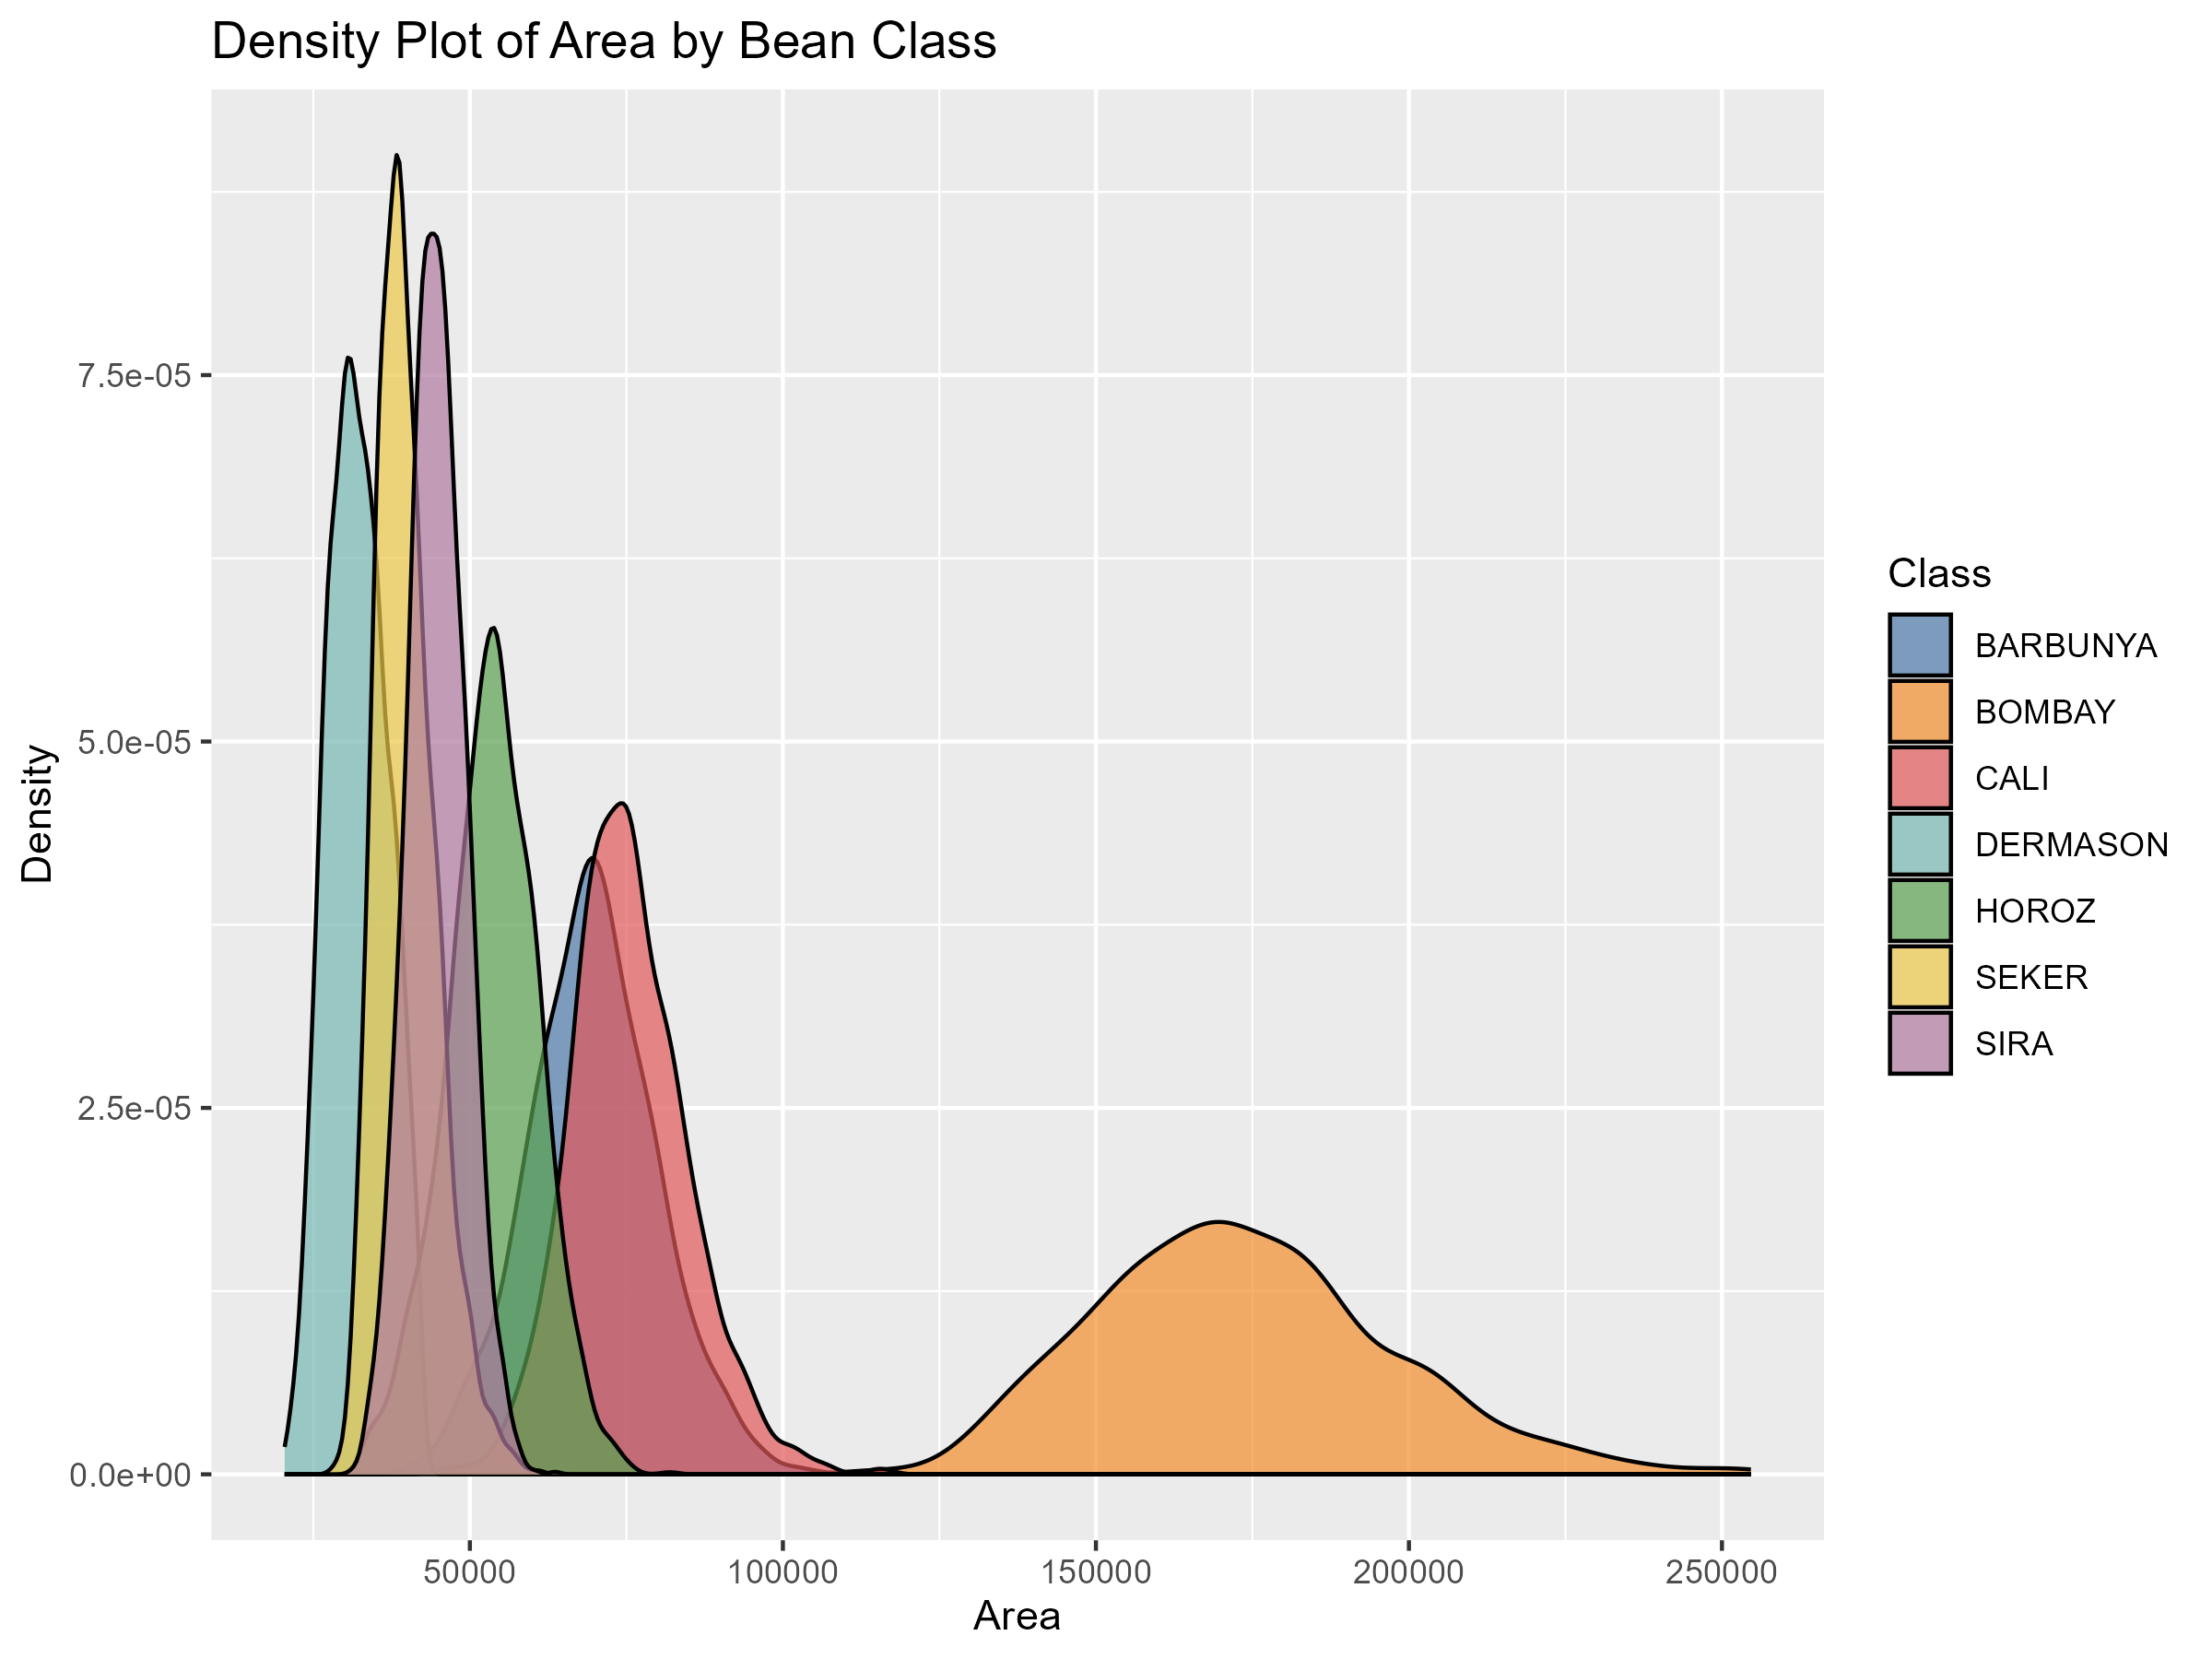
\includegraphics[width=0.8\textwidth]{graphs/density_area_by_class.png}
    \caption{Density Plot of Area by Bean Class}
    \label{fig:density_area}
\end{figure}
This density plot displays the distribution of the area attribute for different bean classes. The x-axis represents the area, and the y-axis indicates the density for each class. Most bean classes, such as BARBUNYA and SIRA, have their area values concentrated between 40,000 and 60,000, while BOMBAY has the widest range, with values extending beyond 100,000. The overlapping curves highlight areas where the bean classes may exhibit similar geometric properties, which may pose challenges in classification.

\newpage

\subsection{Boxplot of Perimeter by Bean Class}
\noindent\textbf{Objective:} This boxplot compares the perimeter values of different bean classes. It addresses: "How does the perimeter distribution differ across various bean types?"

\noindent\textbf{Explanation:} The plot shows the median and spread of perimeter values for each class, revealing outliers and key differences. BOMBAY beans have a wider spread and higher median perimeter values compared to other classes, which can be an important feature for classification.

\begin{figure}[H]
    \centering
    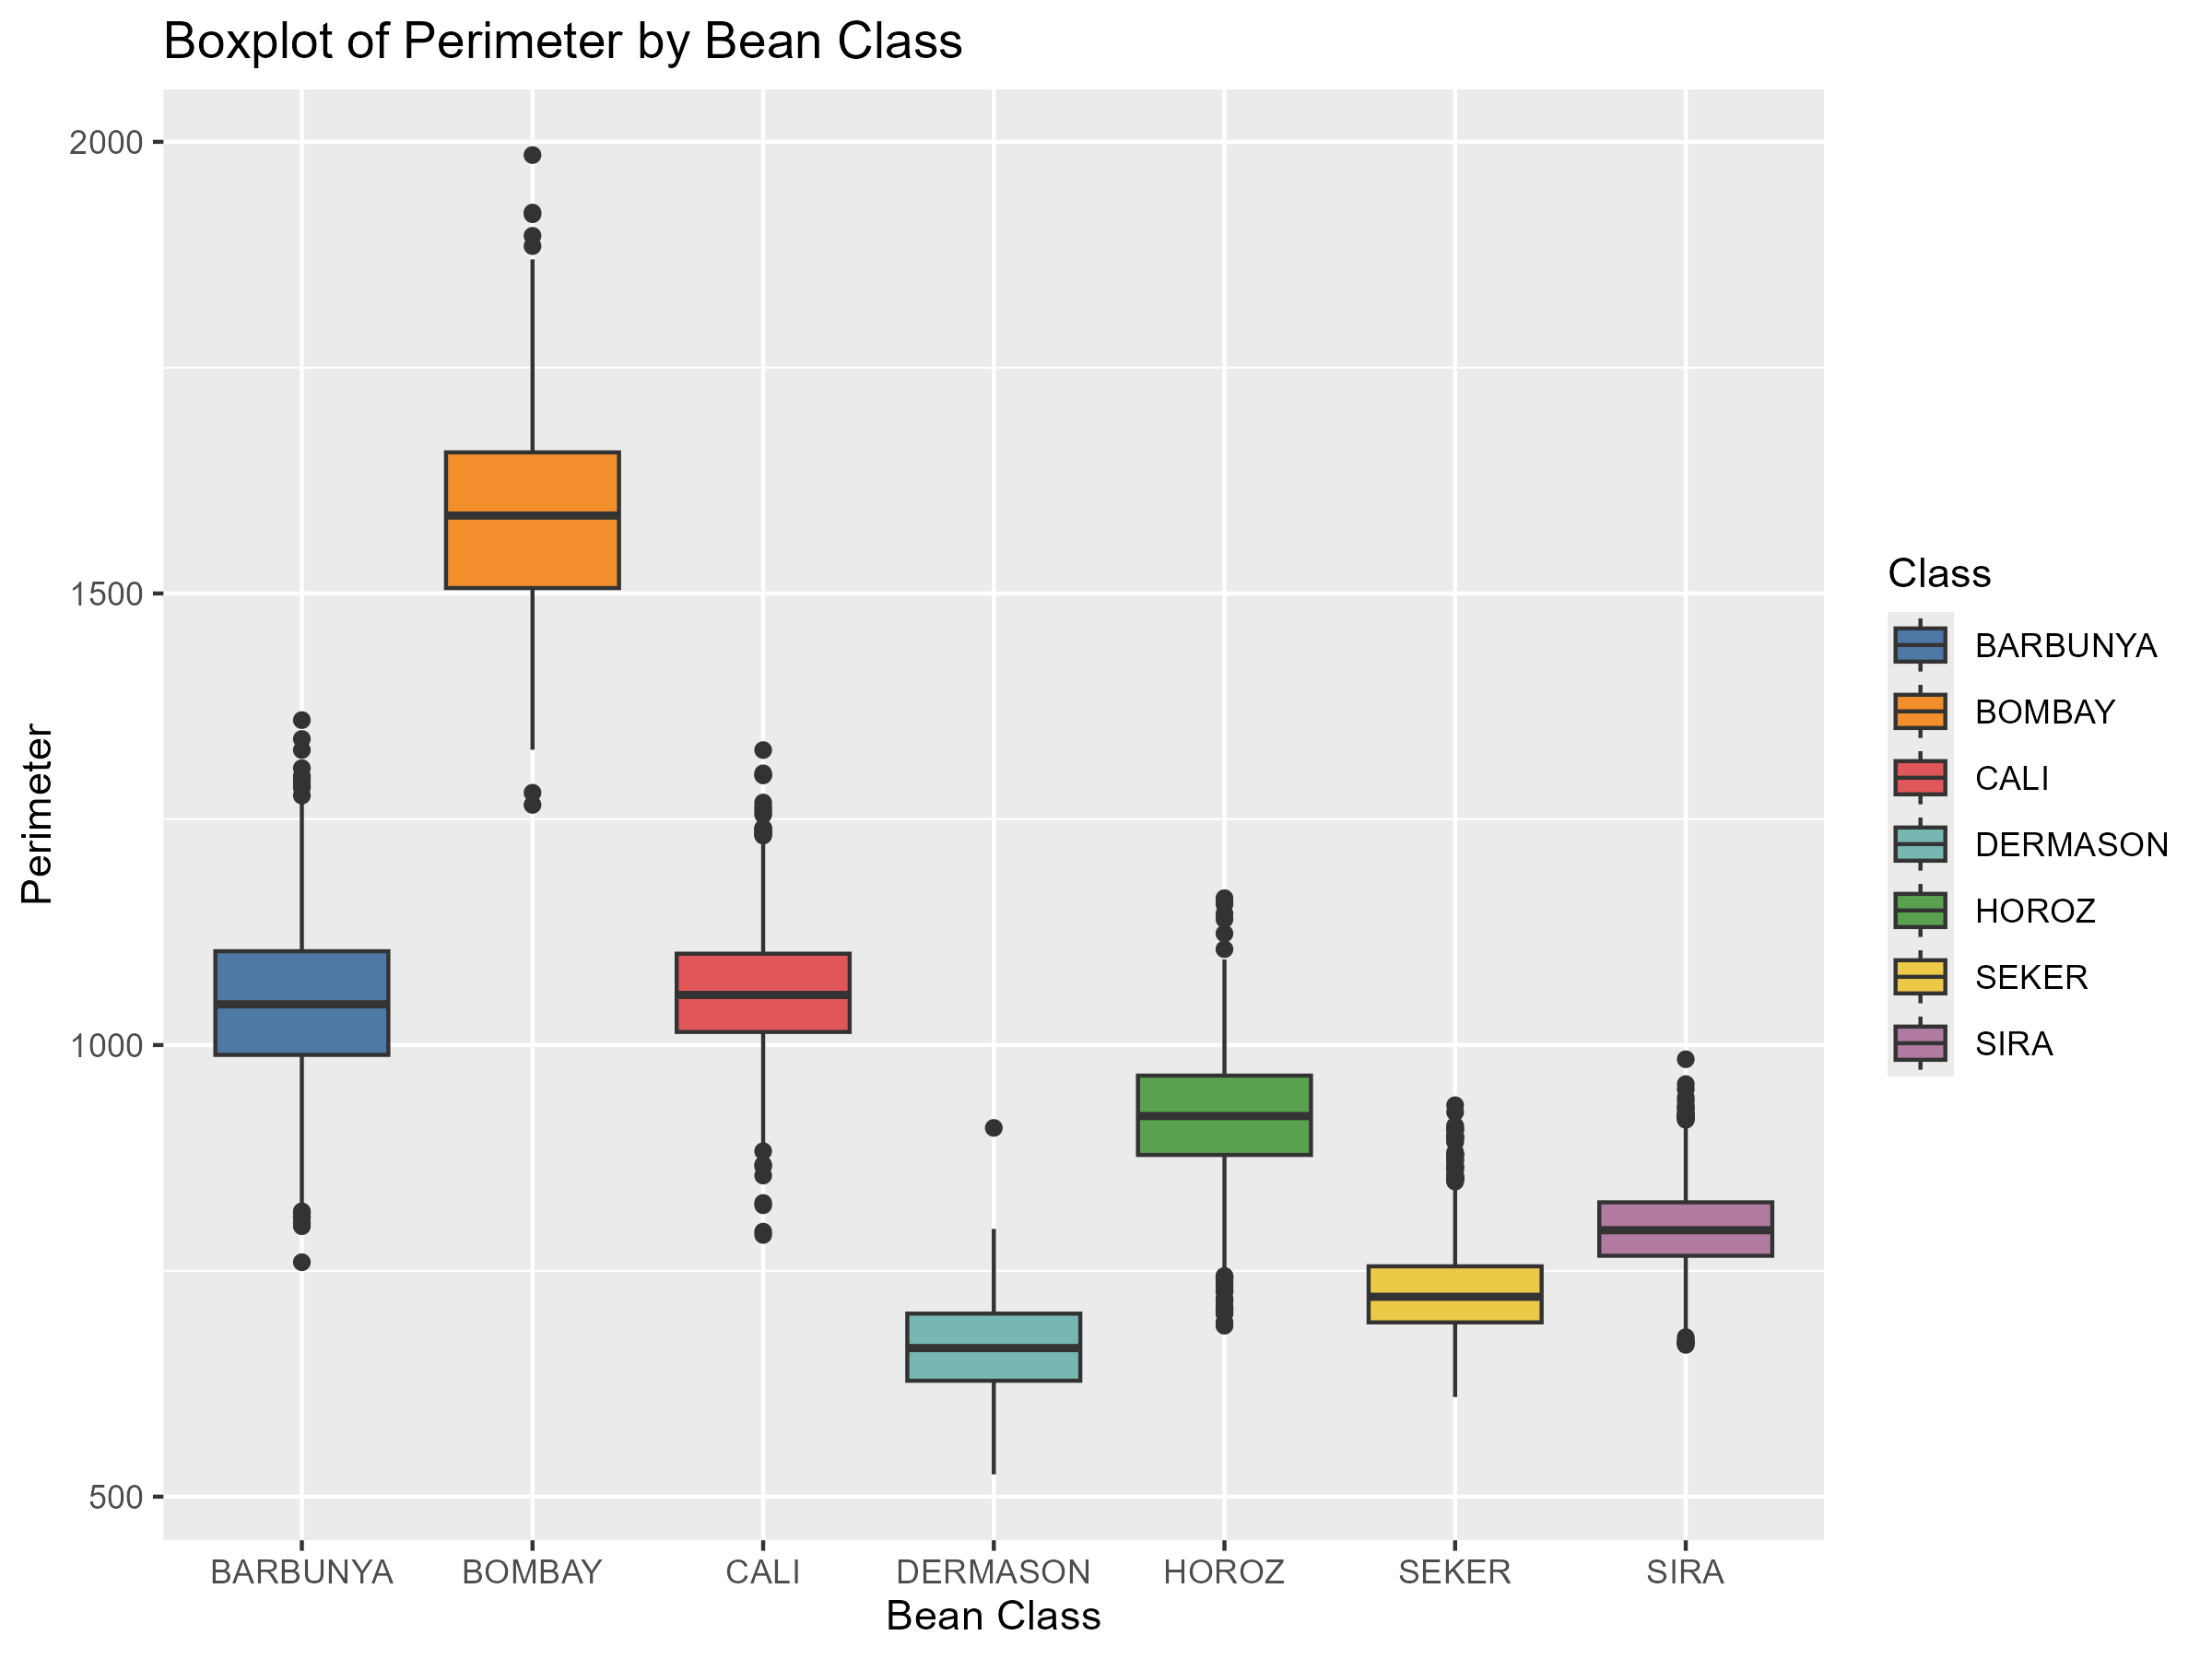
\includegraphics[width=0.8\textwidth]{graphs/boxplot_perimeter.png}
    \caption{Boxplot of Perimeter by Bean Class}
    \label{fig:boxplot_perimeter}
\end{figure}
The boxplot compares the perimeter distributions of each bean class. The x-axis lists the classes, while the y-axis shows the perimeter values. The median and interquartile ranges for each class are displayed. BOMBAY beans have a wider spread and higher median perimeter values, while DERMASON and SIRA have lower perimeter values. Outliers in the dataset are represented by dots. The plot highlights differences in perimeter, a key shape feature, which may help distinguish between bean classes.

\newpage
\subsection{Scatter Plot of Major vs Minor Axis Length}
\noindent\textbf{Objective:} This scatter plot visualizes the relationship between the \textit{Major Axis Length} and \textit{Minor Axis Length}. It answers: "How are the lengths of the major and minor axes related across different bean classes?"

\noindent\textbf{Explanation:} The scatter plot shows that BOMBAY beans are characterized by larger axis lengths, clustering in the upper right. In contrast, SIRA and CALI are more densely packed in the lower left, indicating shorter axis lengths.

\begin{figure}[H]
    \centering
    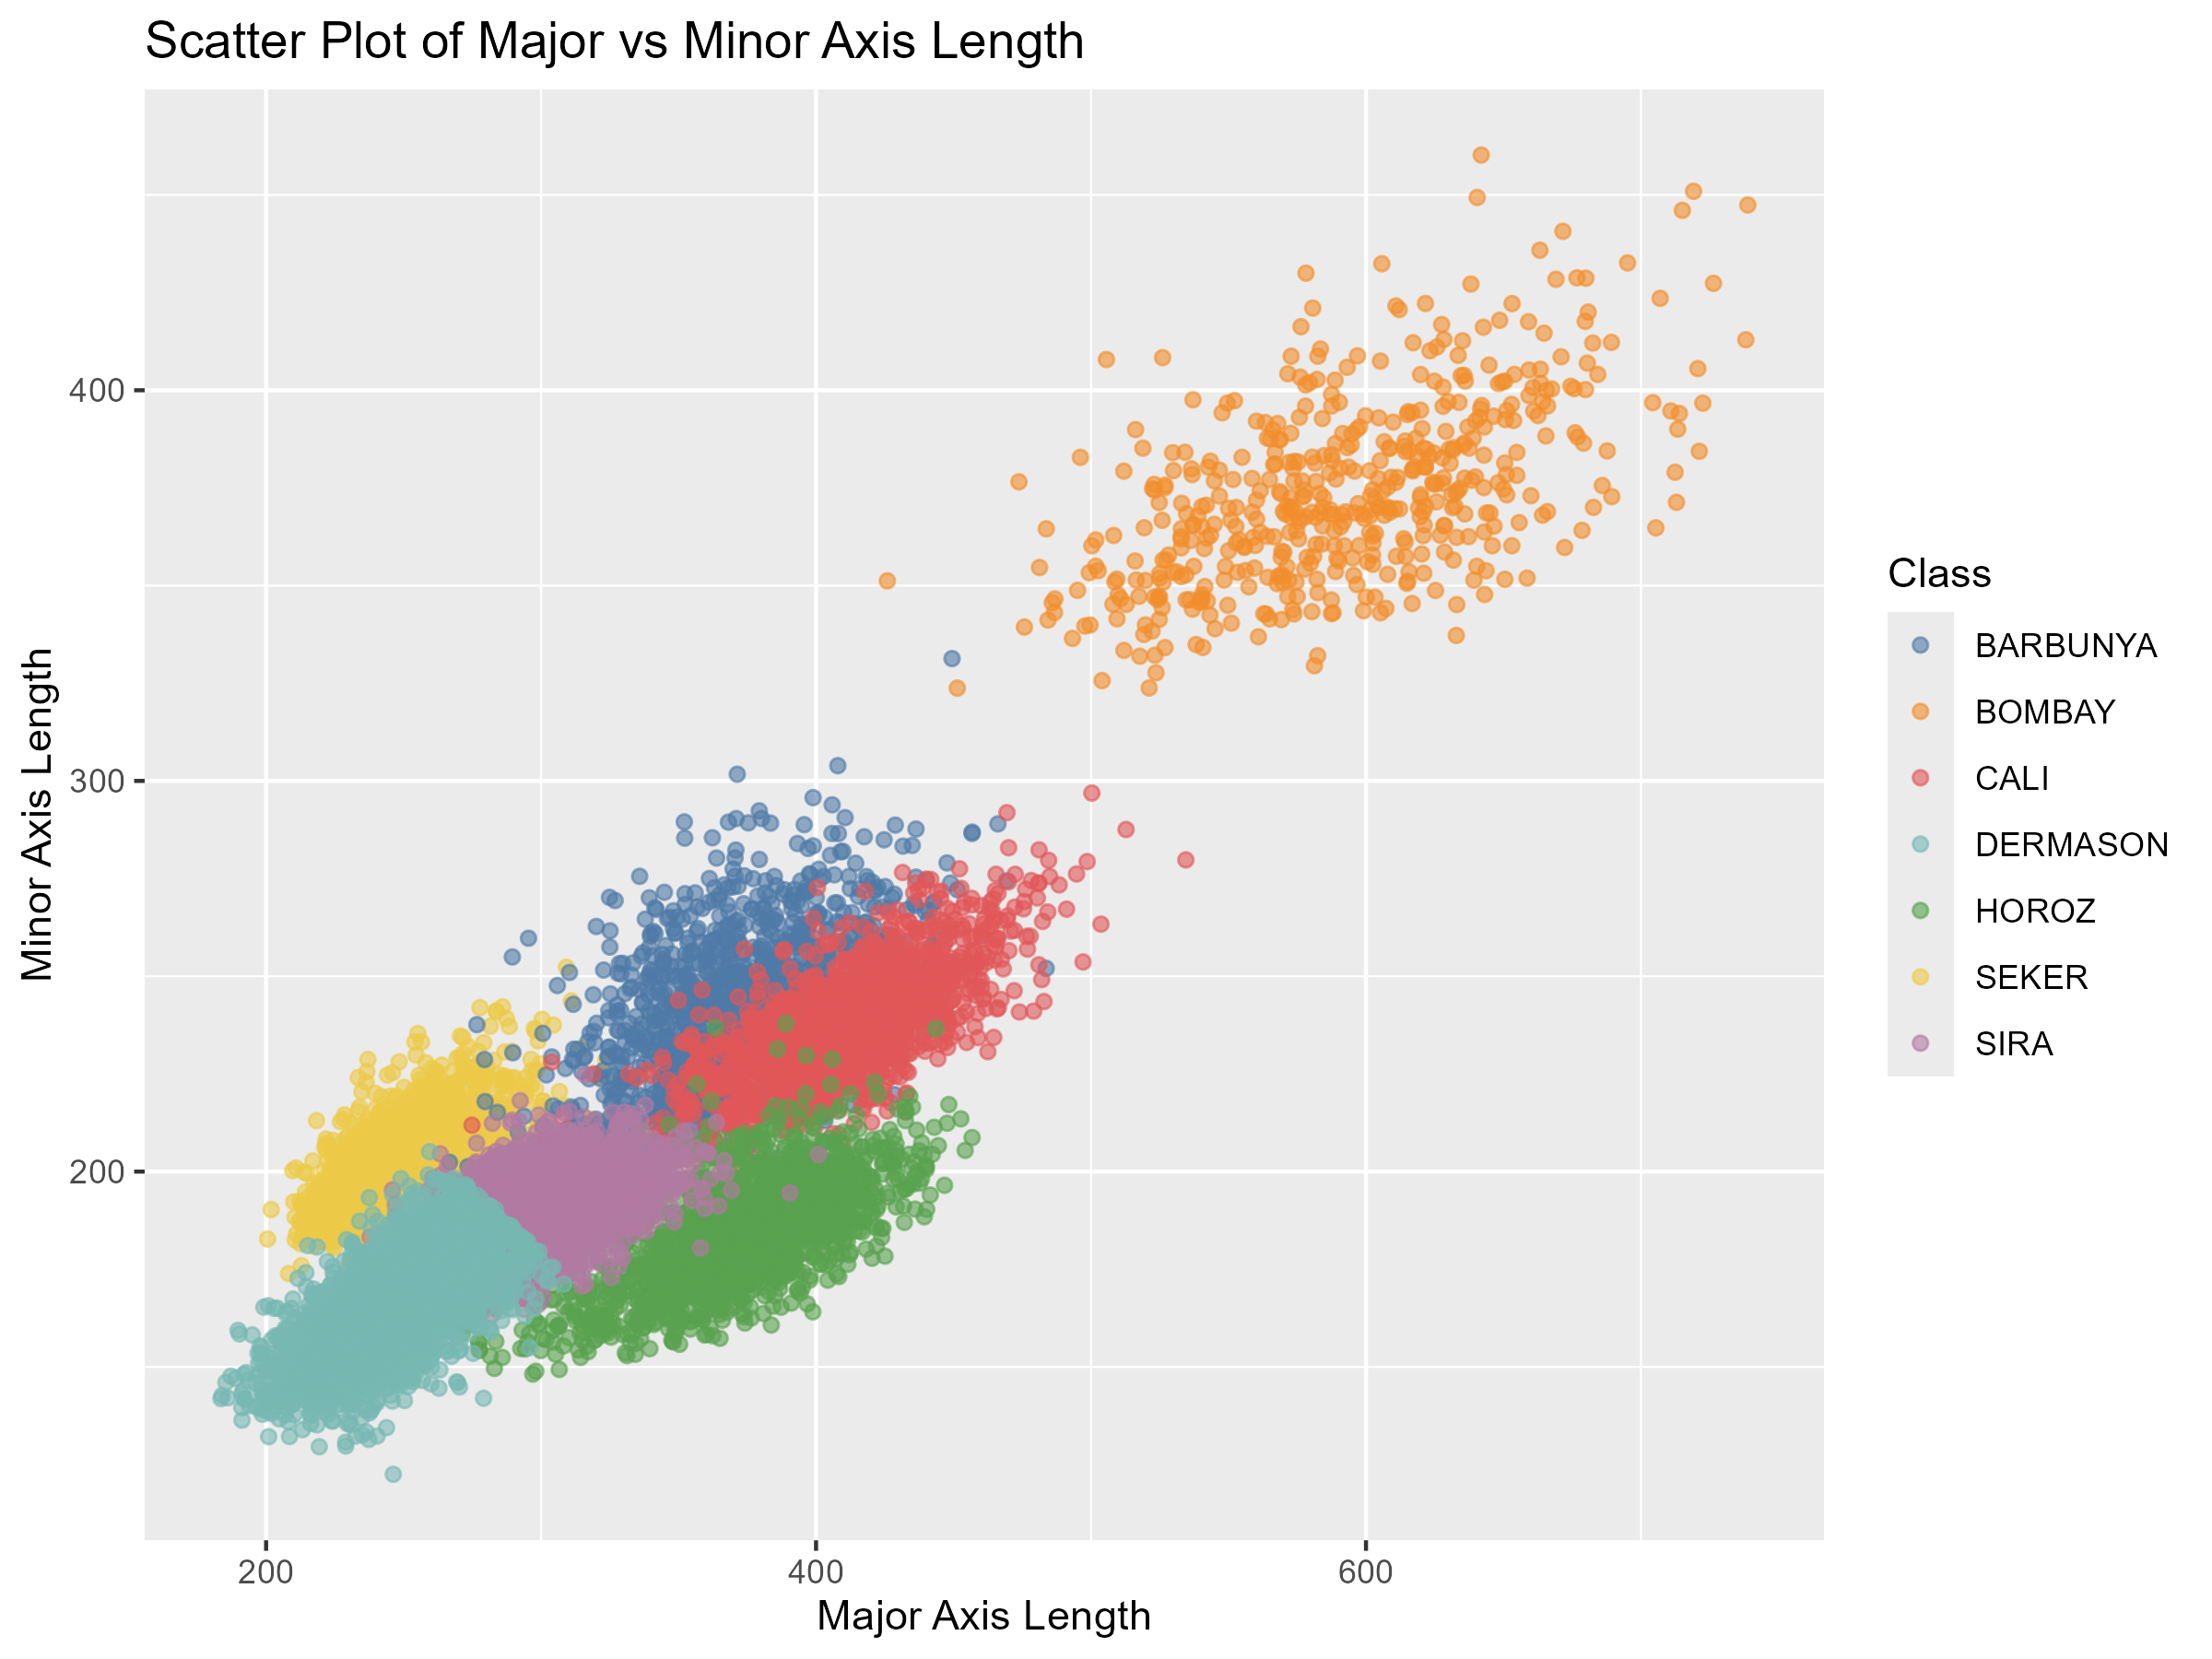
\includegraphics[width=0.8\textwidth]{graphs/scatter_major_minor_axis.png}
    \caption{Scatter Plot of Major vs Minor Axis Length}
    \label{fig:scatter_major_minor}
\end{figure}
This scatter plot illustrates the relationship between the major axis length and minor axis length for different bean classes. Each point represents a single bean instance, with colors indicating the class. BOMBAY beans, characterized by larger axis lengths, cluster in the upper right, while classes like SIRA and CALI are more densely packed in the lower left, indicating shorter axis lengths. This relationship can help in understanding the elongation and overall shape of beans, which are essential in classification tasks.

\newpage

\subsection{Correlation Heatmap}
\noindent\textbf{Objective:} The heatmap illustrates the correlations between different numerical features, answering the question: "Which features have the strongest correlations, and how can this information guide feature selection?"

\noindent\textbf{Explanation:} The heatmap indicates strong positive correlations between features such as \textit{Area}, \textit{Perimeter}, and \textit{Major Axis Length}. This suggests that some features may contain overlapping information, and feature selection techniques may be applied to reduce redundancy.

\begin{figure}[H]
    \centering
    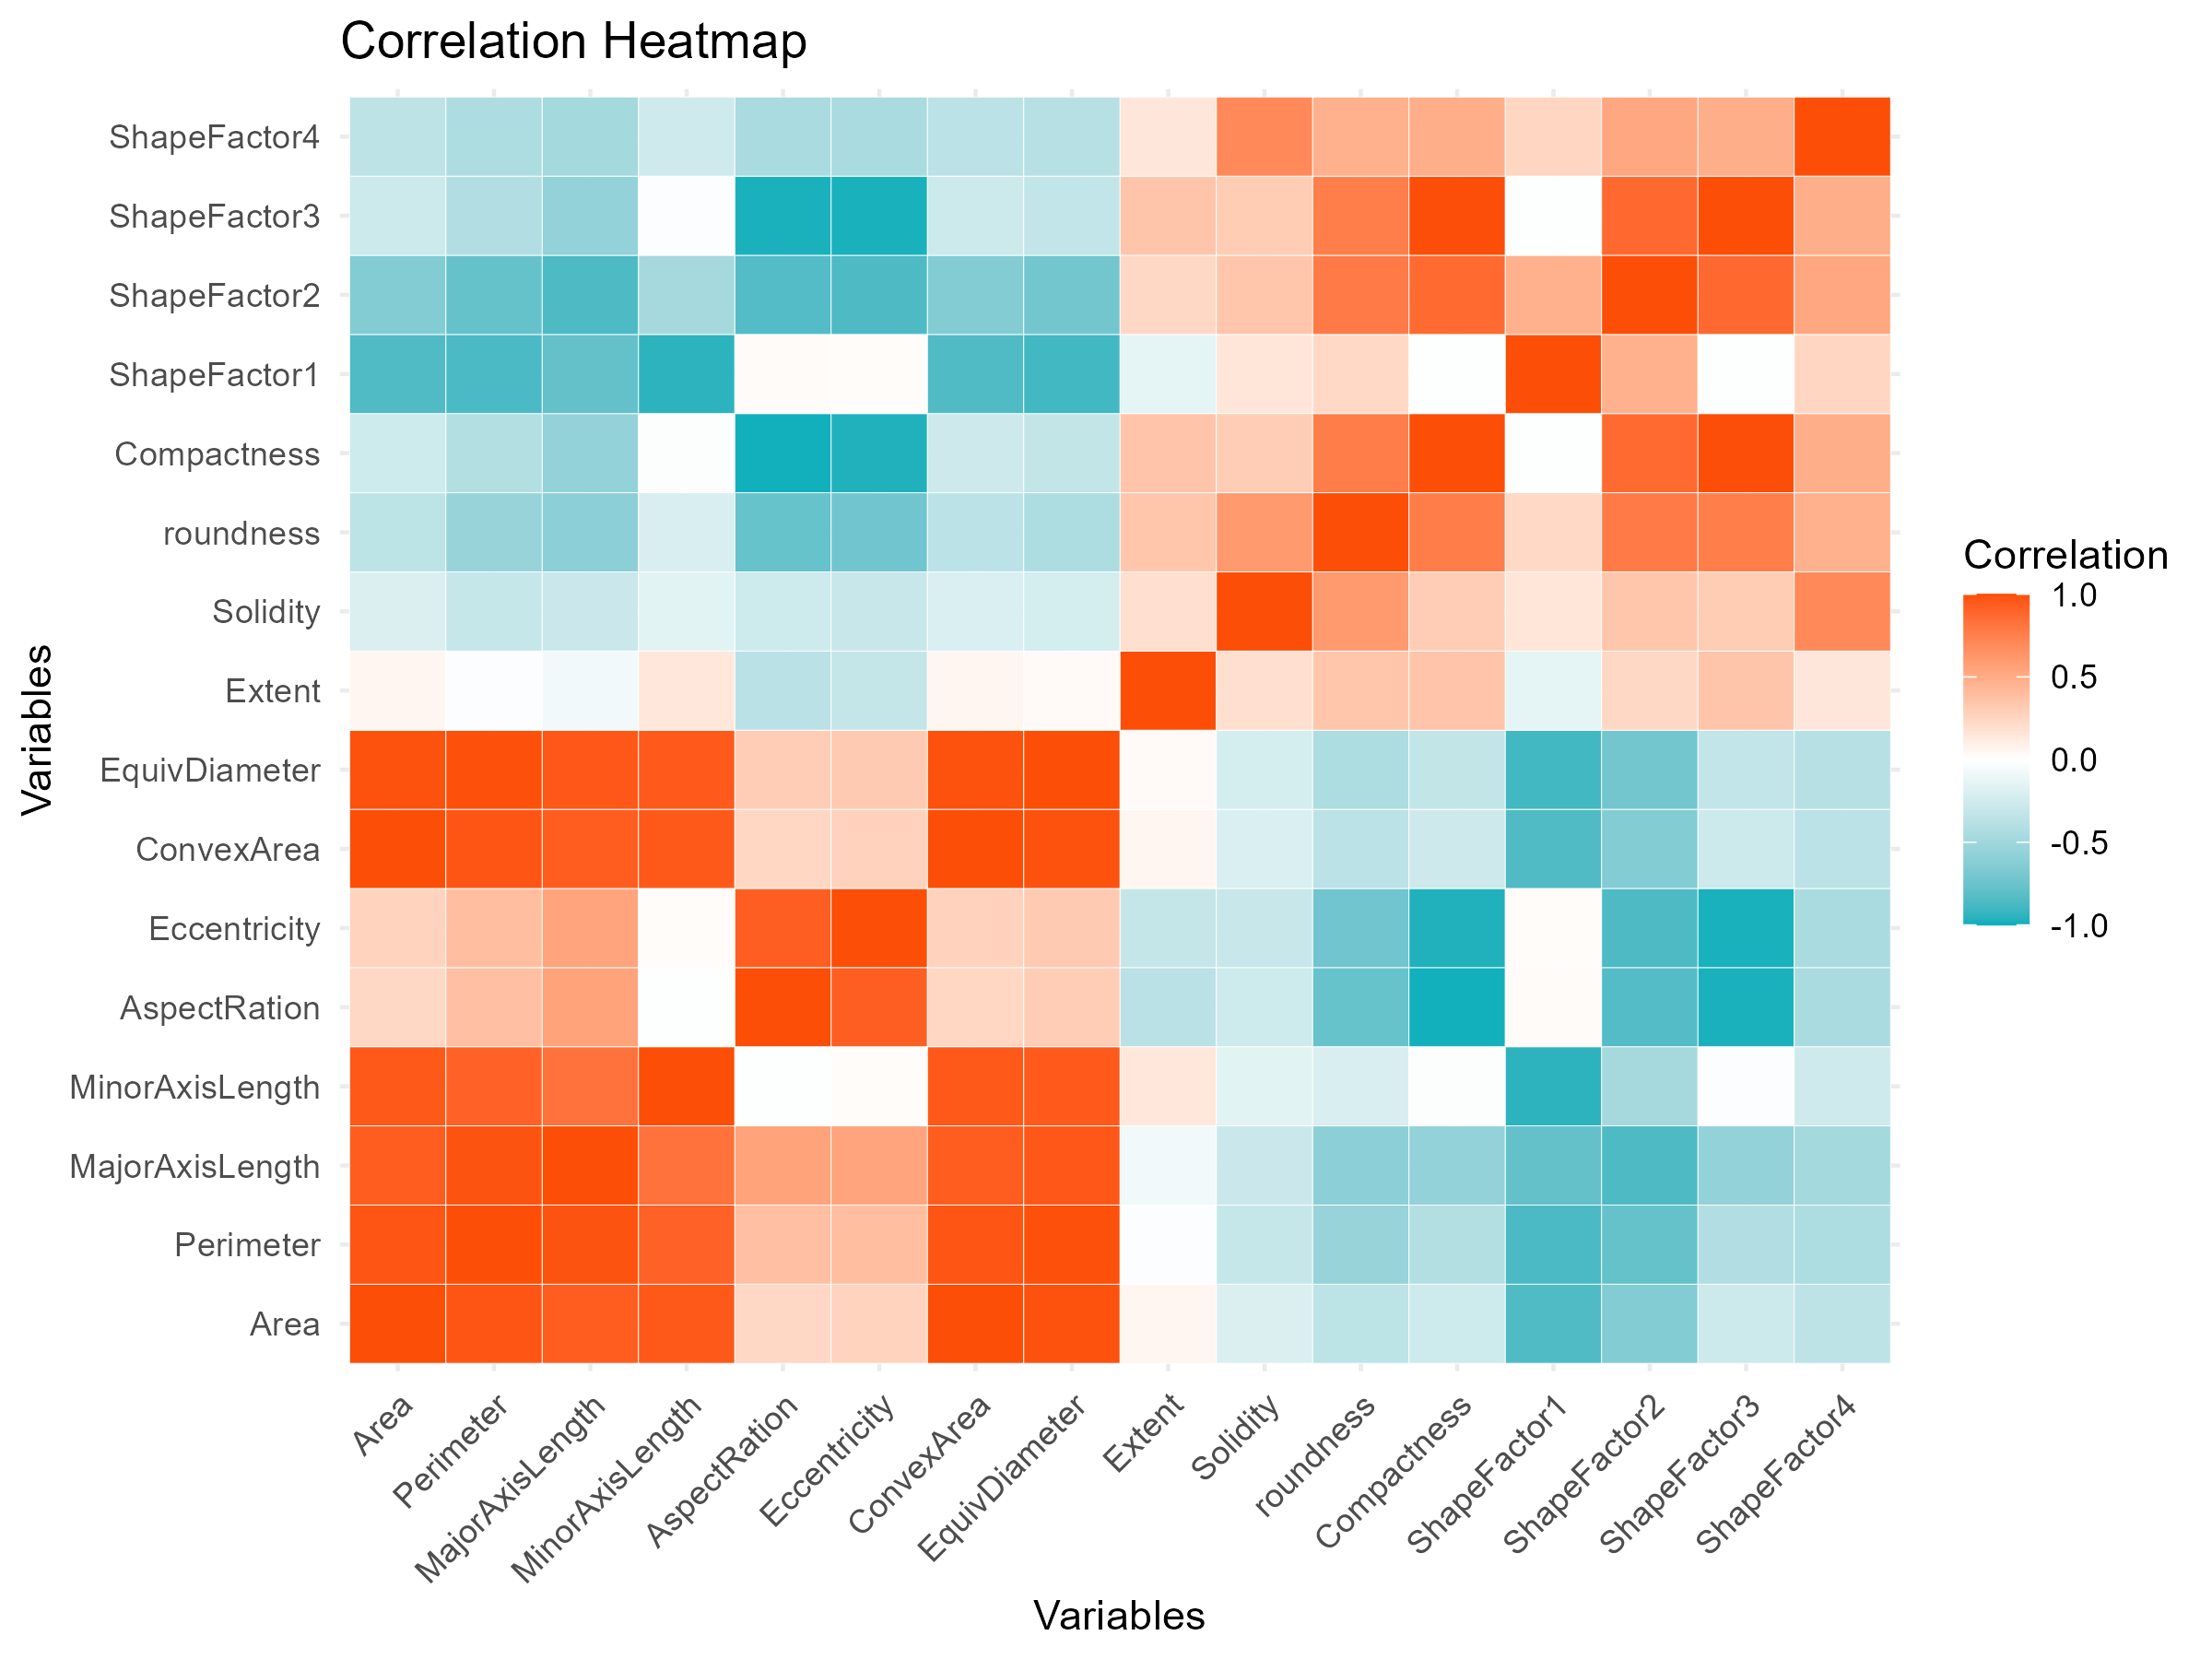
\includegraphics[width=0.8\textwidth]{graphs/correlation_heatmap.png}
    \caption{Correlation Heatmap}
    \label{fig:correlation_heatmap}
\end{figure}
The heatmap above shows correlations between the numerical variables in the dataset. Darker colors represent stronger correlations. Variables such as area, perimeter, major axis length, and minor axis length show strong positive correlations, indicating that as one increases, so do the others. Negative correlations, while weaker, can also be seen. This heatmap helps identify key relationships between features and is useful for feature selection in predictive modeling.

\newpage

\subsection{Scatter Plot of Area vs Perimeter}
\noindent\textbf{Objective:} This scatter plot examines the relationship between the \textit{Area} and \textit{Perimeter} of beans, answering: "Is there a strong correlation between area and perimeter?"

\noindent\textbf{Explanation:} The plot reveals a positive correlation between \textit{Area} and \textit{Perimeter}, meaning that larger beans generally have larger perimeters. BOMBAY beans appear in the upper right, indicating that they have larger sizes.

\begin{figure}[H]
    \centering
    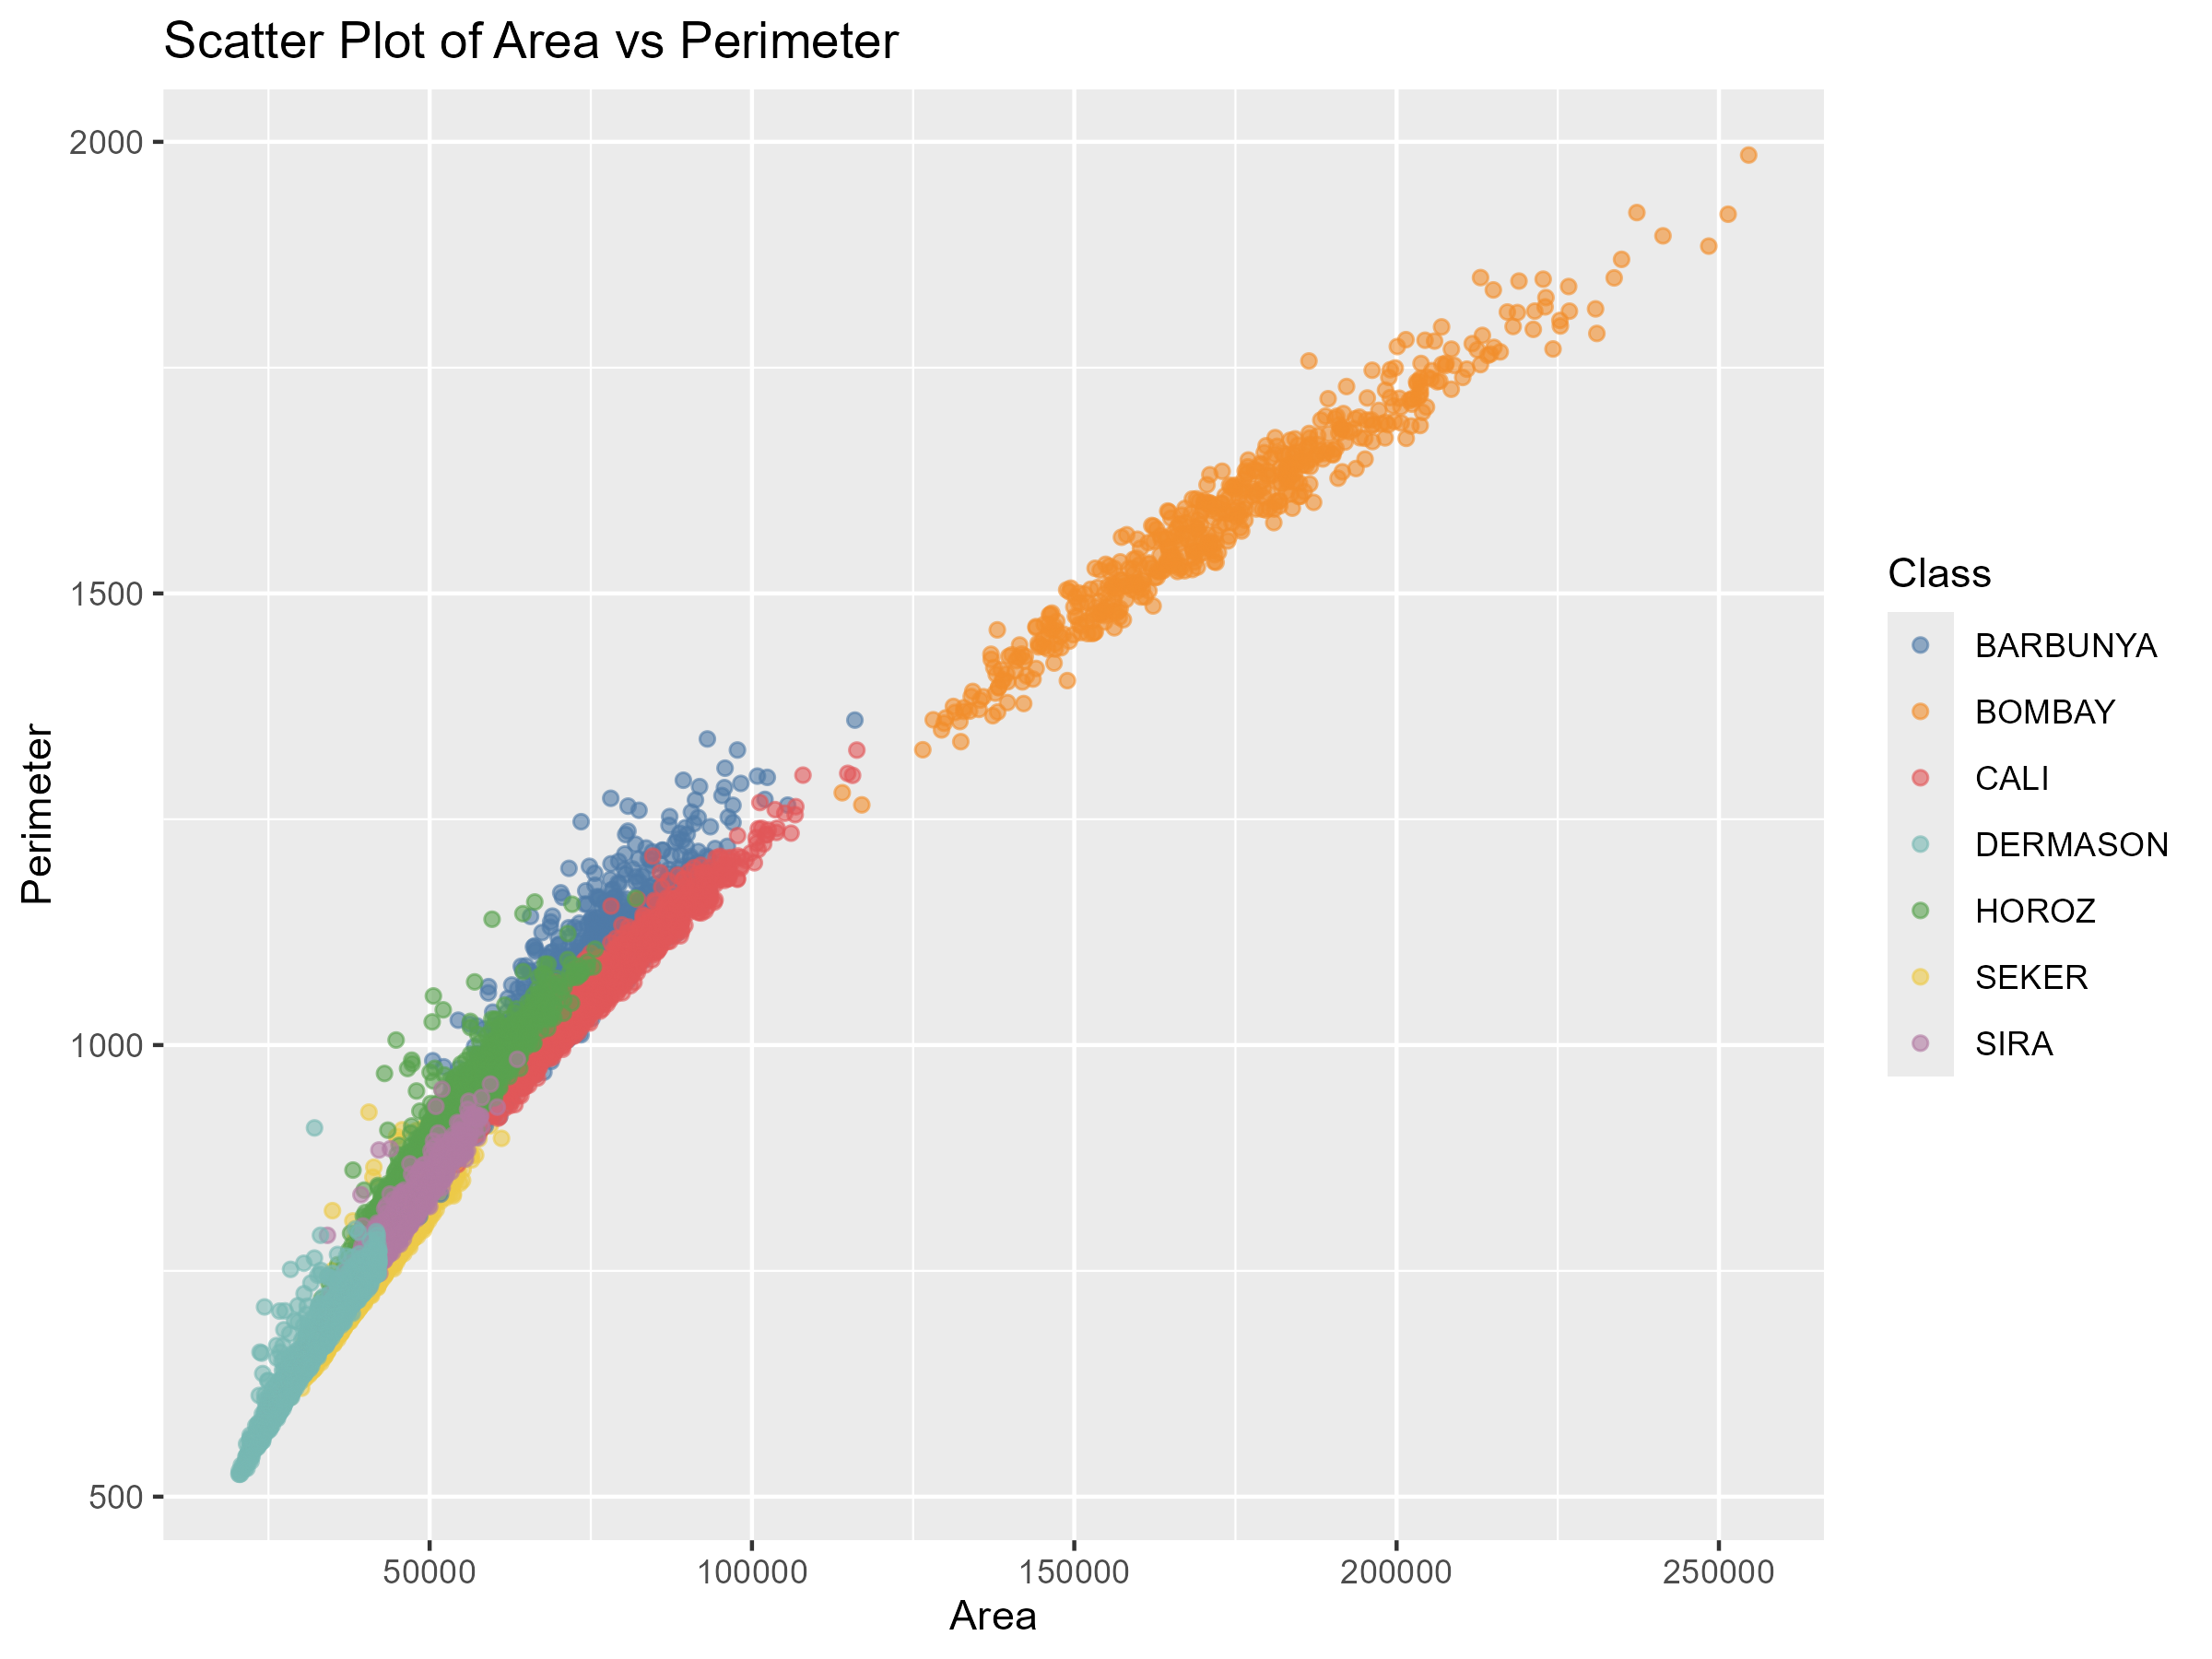
\includegraphics[width=0.8\textwidth]{graphs/scatter_area_perimeter.png}
    \caption{Scatter Plot of Area vs Perimeter}
    \label{fig:scatter_area_perimeter}
\end{figure}
The scatter plot shows a clear positive correlation between area and perimeter, meaning that as the area of a bean increases, so does its perimeter. BOMBAY beans, shown in orange, have the largest areas and perimeters, while other classes cluster around smaller values. This strong correlation indicates that larger beans tend to be more elongated, and both features can be important for classifying bean types.

\newpage

\subsection{Density Plot of Compactness by Bean Class}
\noindent\textbf{Objective:} This plot explores how the \textit{Compactness} attribute varies across different bean classes. It answers the question: "Do certain bean classes exhibit higher compactness, indicating a more regular shape?"

\noindent\textbf{Explanation:} The density curves show that SEKER and DERMASON beans exhibit higher compactness values, indicating more regular shapes compared to other classes.

\begin{figure}[H]
    \centering
    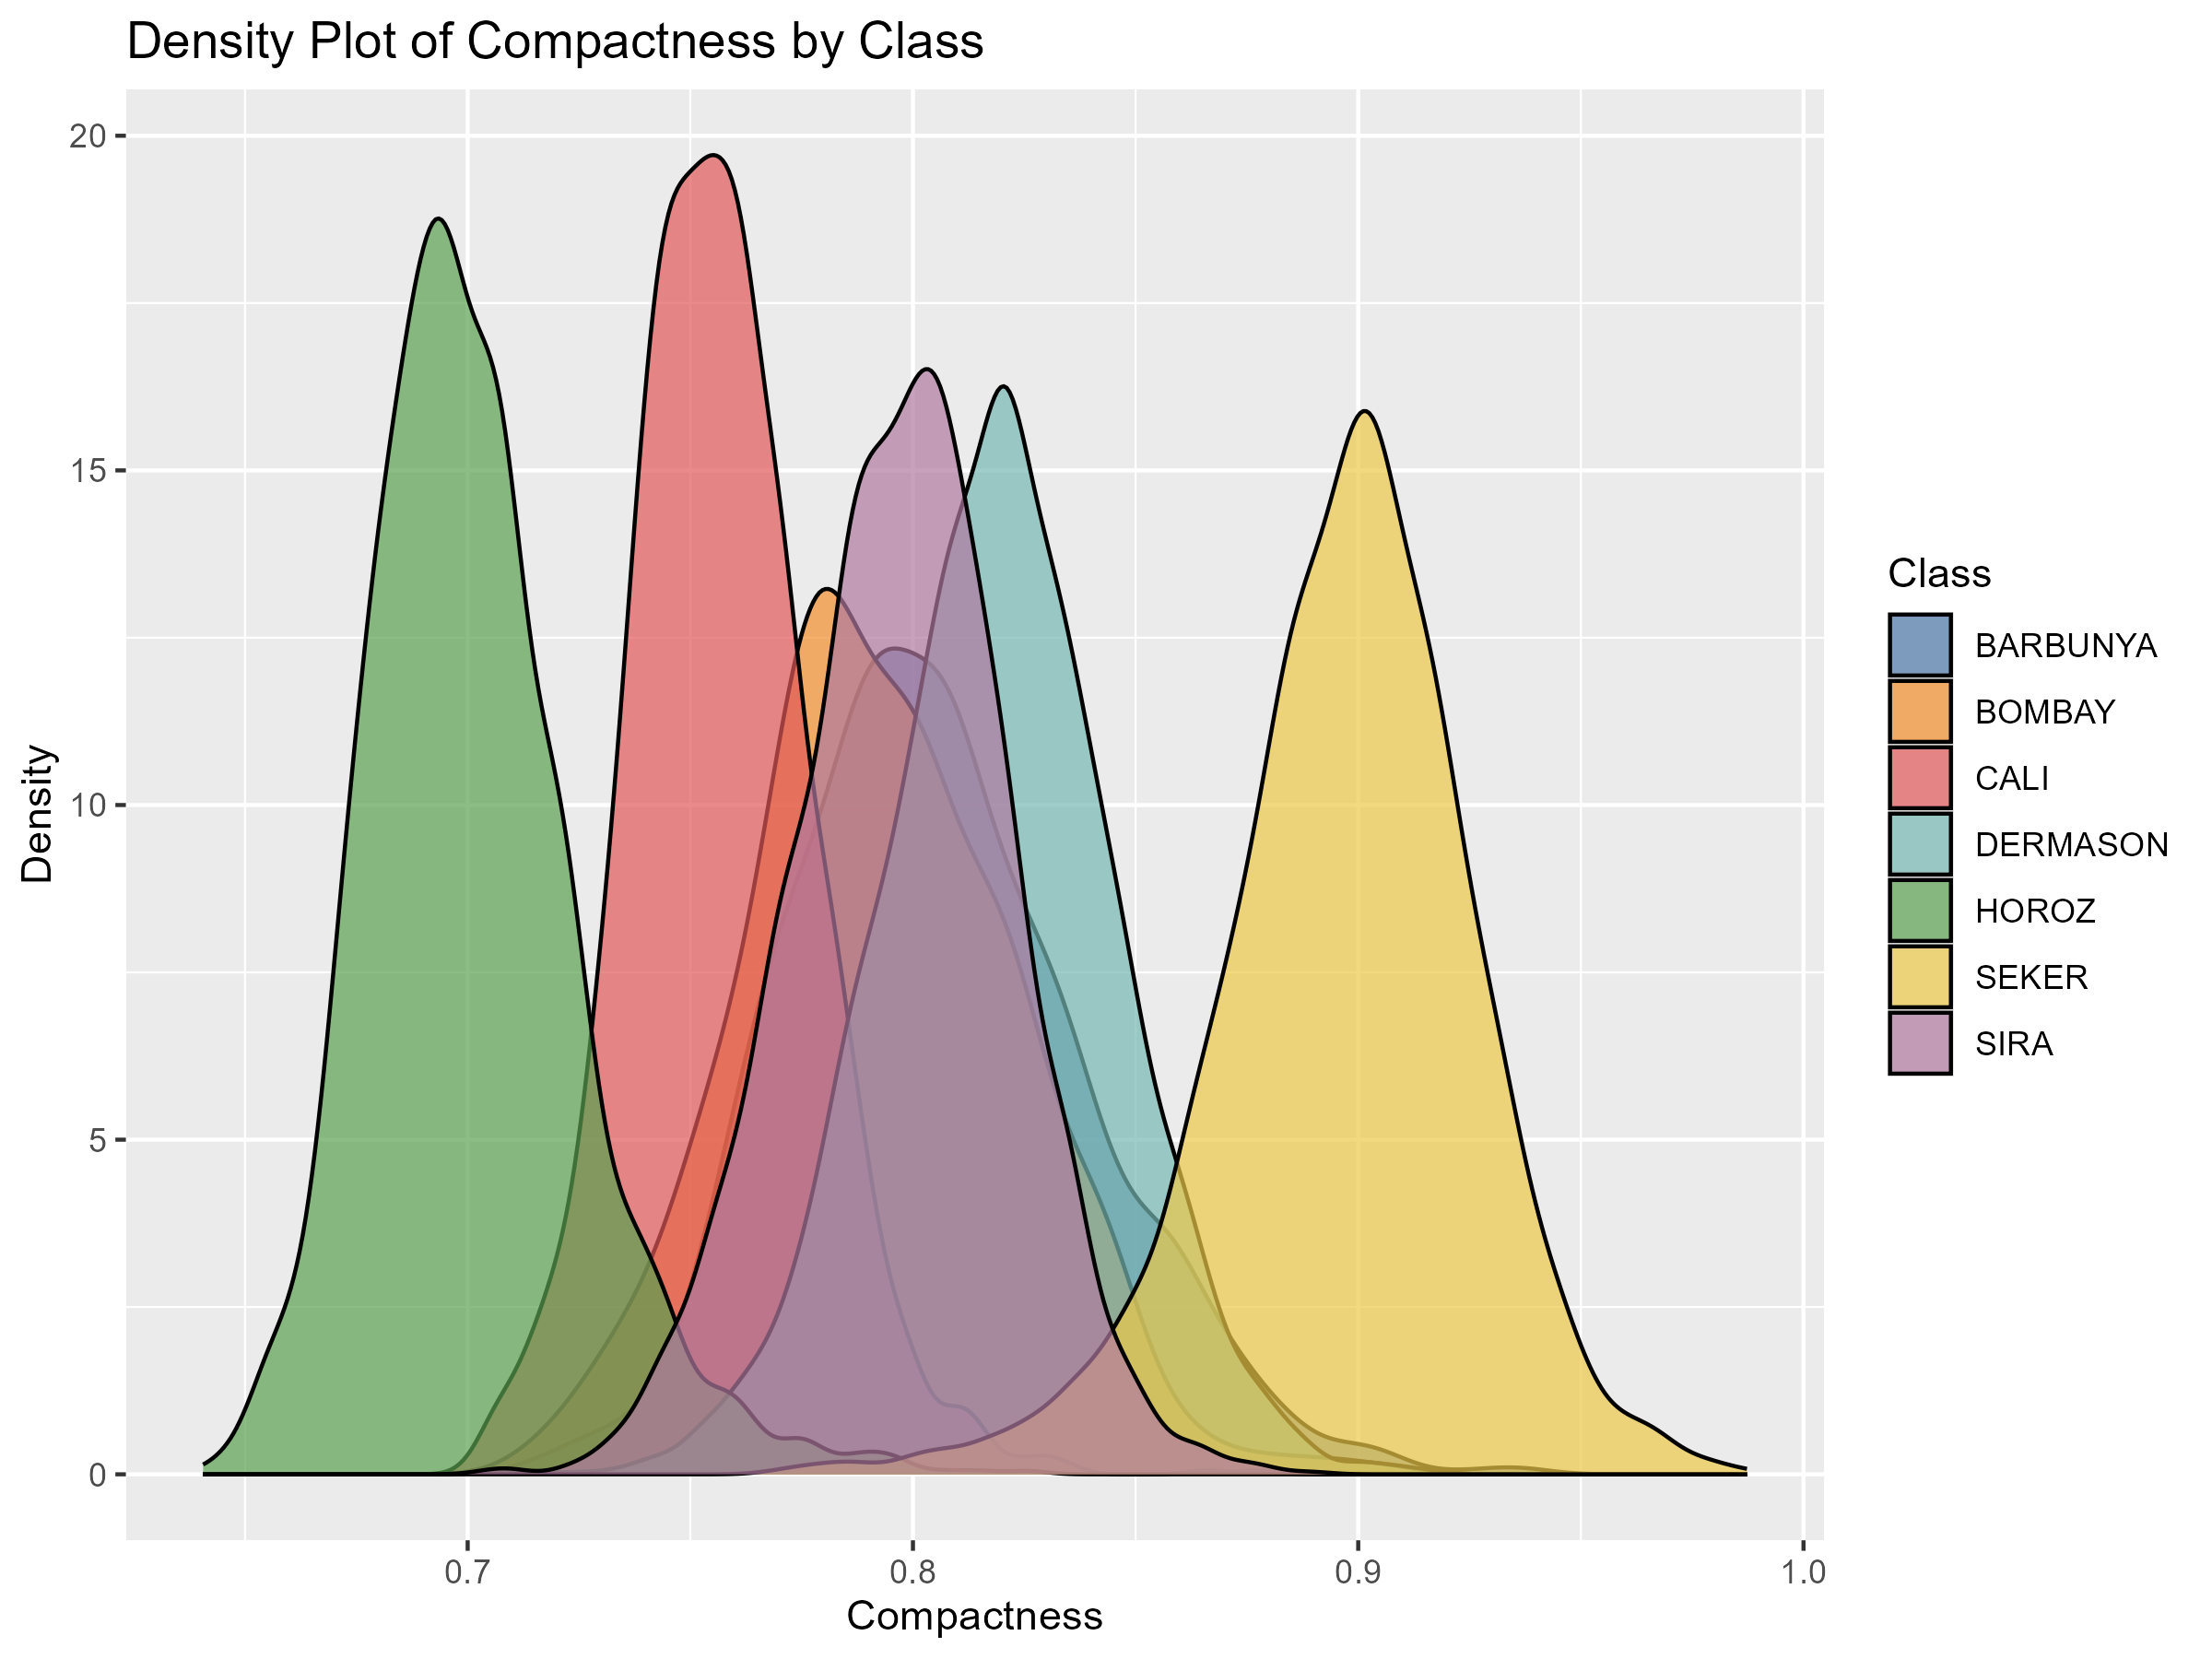
\includegraphics[width=0.8\textwidth]{graphs/density_compactness.png}
    \caption{Density Plot of Compactness by Bean Class}
    \label{fig:density_compactness}
\end{figure}
This density plot illustrates the distribution of compactness for different bean classes. The x-axis represents compactness values, while the y-axis shows the density. Classes like SEKER and DERMASON exhibit higher compactness, while HOROZ and CALI have broader distributions. Compactness is an important feature for identifying how closely packed or regular a bean's shape is, which helps differentiate between similar-sized beans.
\newpage

\subsection{Boxplot of Eccentricity by Bean Class}
\noindent\textbf{Objective:} This boxplot illustrates how the \textit{Eccentricity} of beans differs across classes. It addresses: "Which bean classes are more elongated?"

\noindent\textbf{Explanation:} The plot shows that HOROZ and SIRA beans have higher median eccentricity values, indicating that they are more elongated, while SEKER beans appear more circular.

\begin{figure}[H]
    \centering
    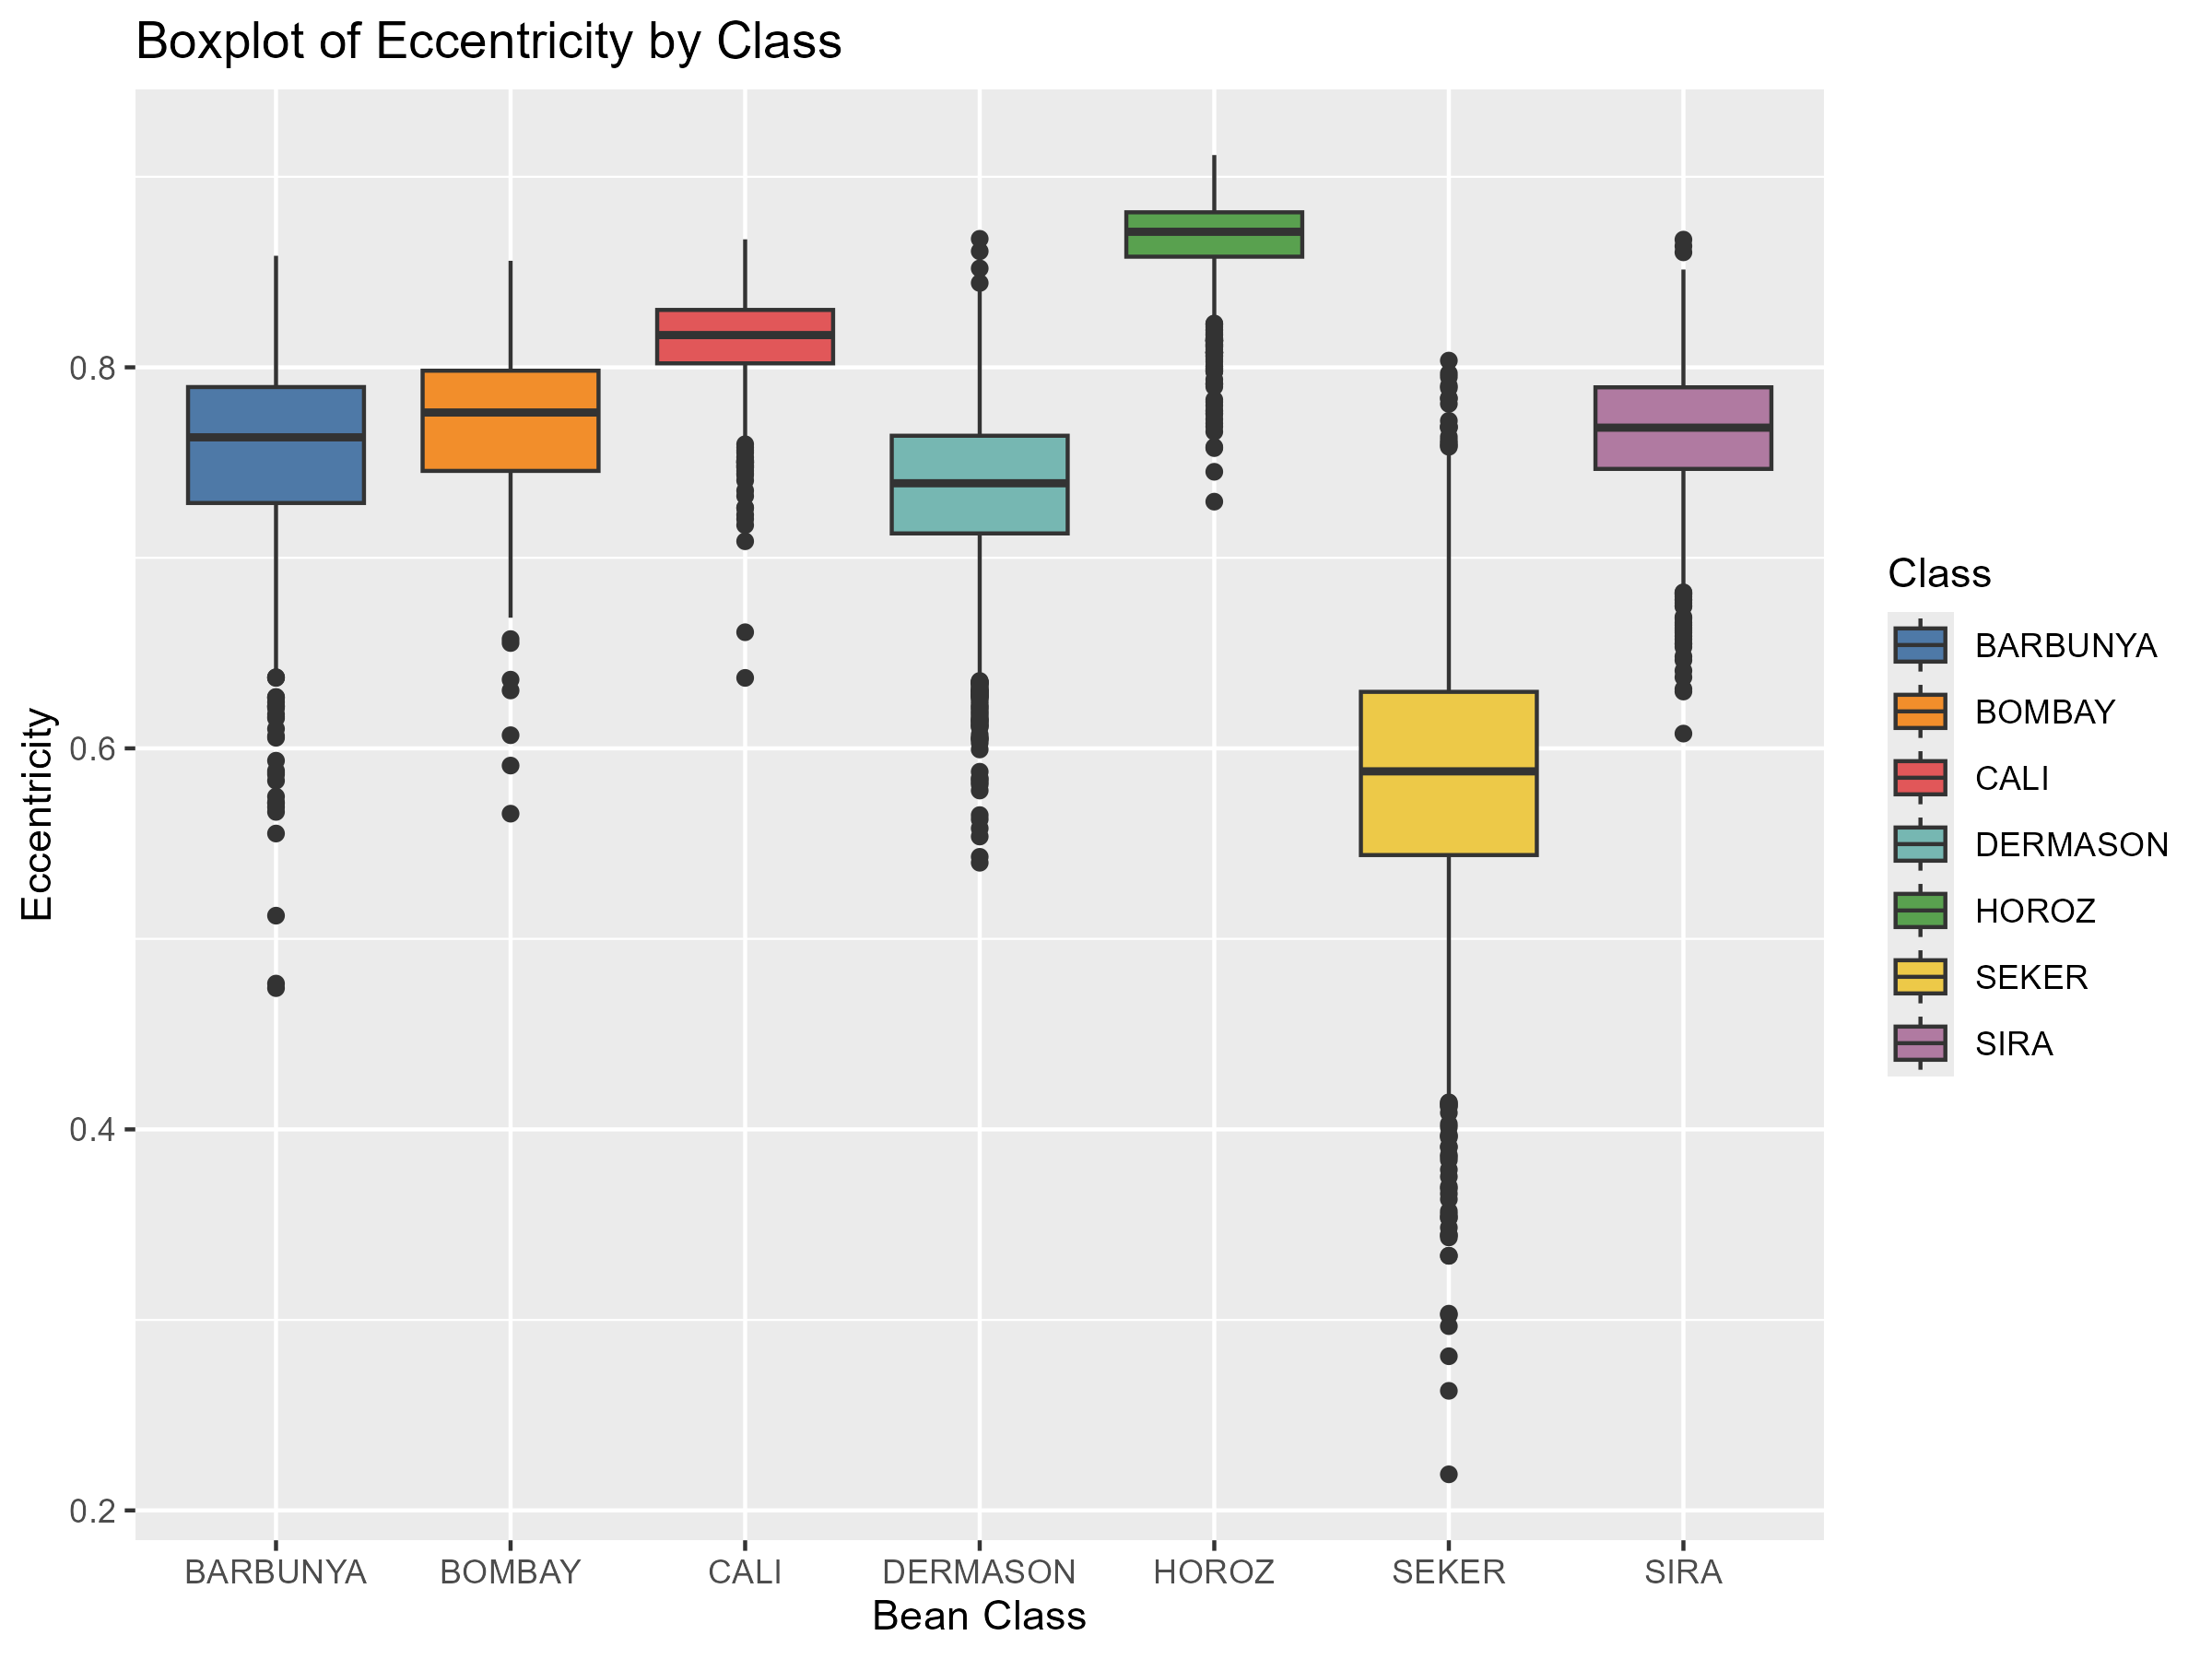
\includegraphics[width=0.8\textwidth]{graphs/boxplot_eccentricity.png}
    \caption{Boxplot of Eccentricity by Bean Class}
    \label{fig:boxplot_eccentricity}
\end{figure}
The boxplot above compares the eccentricity distributions of different bean classes. Eccentricity measures how elongated a bean is, with higher values indicating greater elongation. HOROZ and SIRA beans have higher median eccentricity values, while SEKER beans are more circular. The plot helps identify which classes tend to be more elongated, which can be crucial in distinguishing between classes based on shape.


\newpage
\subsection{Scatter Plot of Roundness vs Compactness}
\noindent\textbf{Objective:} This scatter plot analyzes the relationship between \textit{Roundness} and \textit{Compactness}. It answers the question: "Is there a correlation between the roundness and compactness of beans?"

\noindent\textbf{Explanation:} The scatter plot reveals a positive relationship between \textit{Roundness} and \textit{Compactness}, with more rounded beans also showing higher compactness. SEKER beans tend to exhibit higher values for both attributes.

\begin{figure}[H]
    \centering
    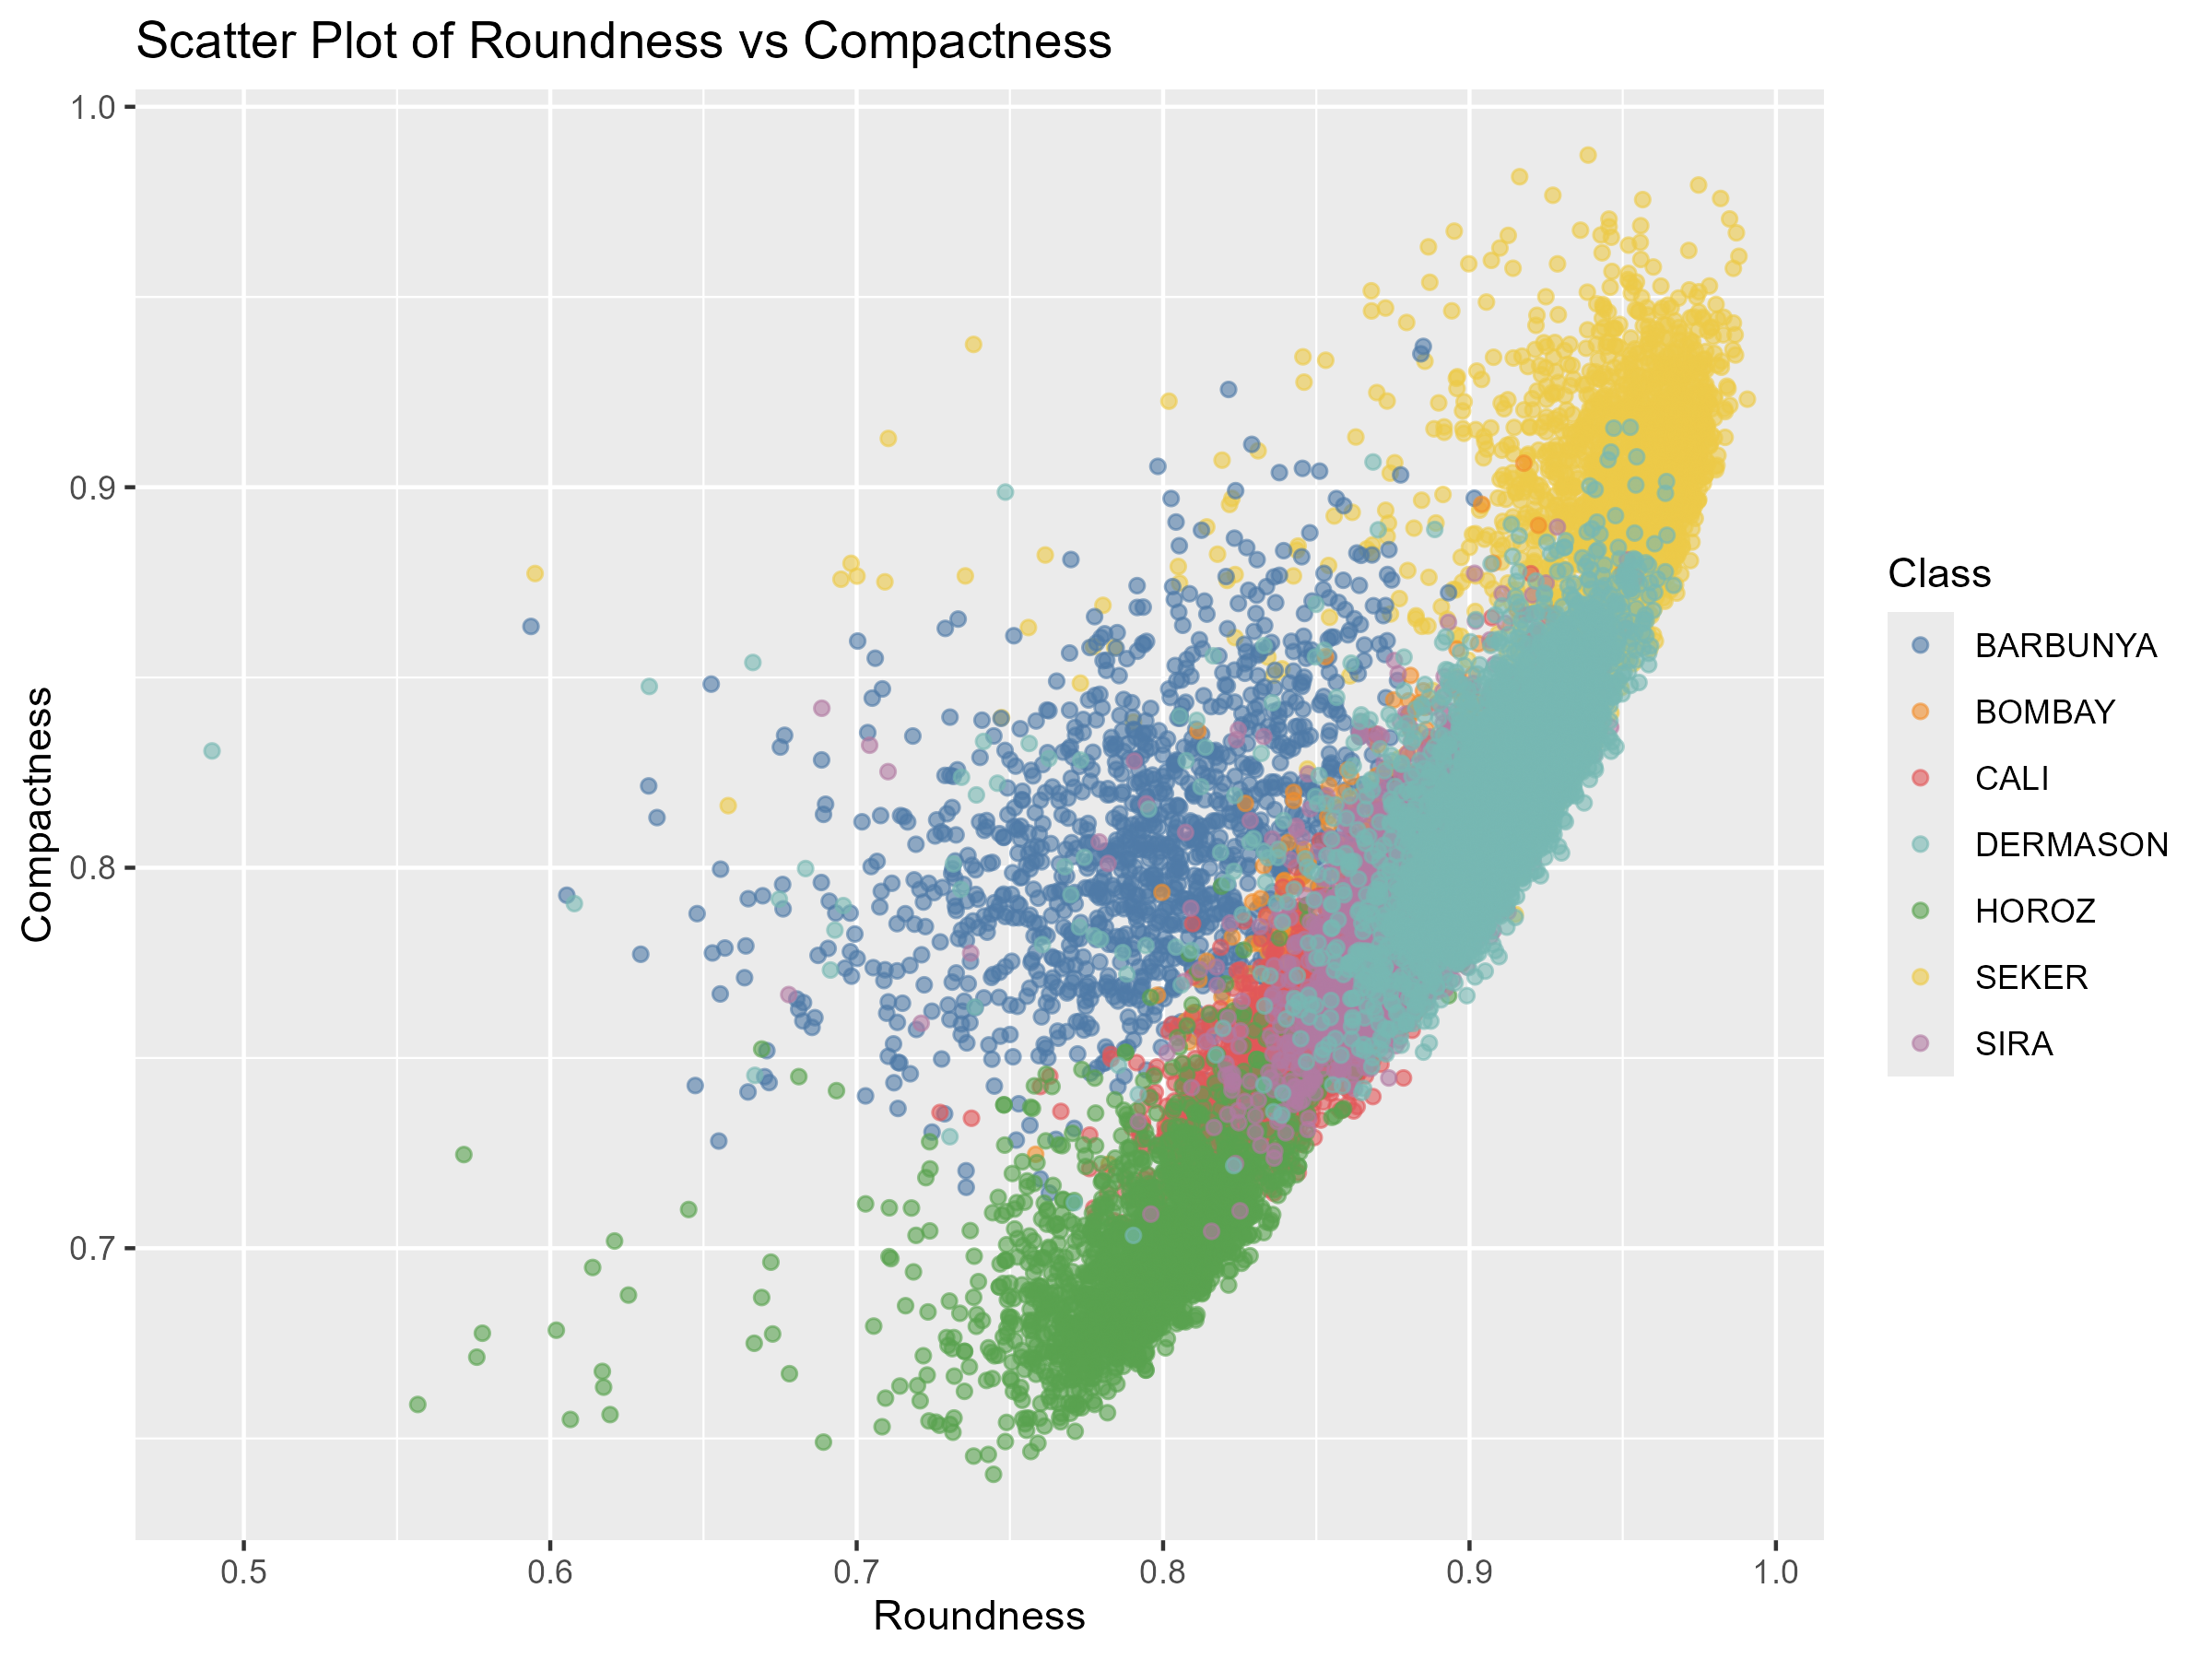
\includegraphics[width=0.8\textwidth]{graphs/scatter_roundness_compactness.png}
    \caption{Scatter Plot of Roundness vs Compactness}
    \label{fig:scatter_roundness_compactness}
\end{figure}
This scatter plot shows the relationship between roundness and compactness for different bean classes. The x-axis represents roundness, while the y-axis shows compactness. There is a clear positive correlation between these two attributes, meaning as roundness increases, compactness also tends to increase. SEKER beans, which are both highly round and compact, appear in the upper right, while elongated beans like BOMBAY cluster in the lower-left quadrant.

\newpage

\subsection{Violin Plot of Aspect Ratio by Bean Class}
\noindent\textbf{Objective:} This violin plot displays the distribution of the \textit{Aspect Ratio} for different bean classes, answering: "How does the aspect ratio vary among bean types?"

\noindent\textbf{Explanation:} The plot shows that certain classes, such as HOROZ, exhibit a wider spread in aspect ratio, while other classes like SEKER have a more compact distribution.

\begin{figure}[H]
    \centering
    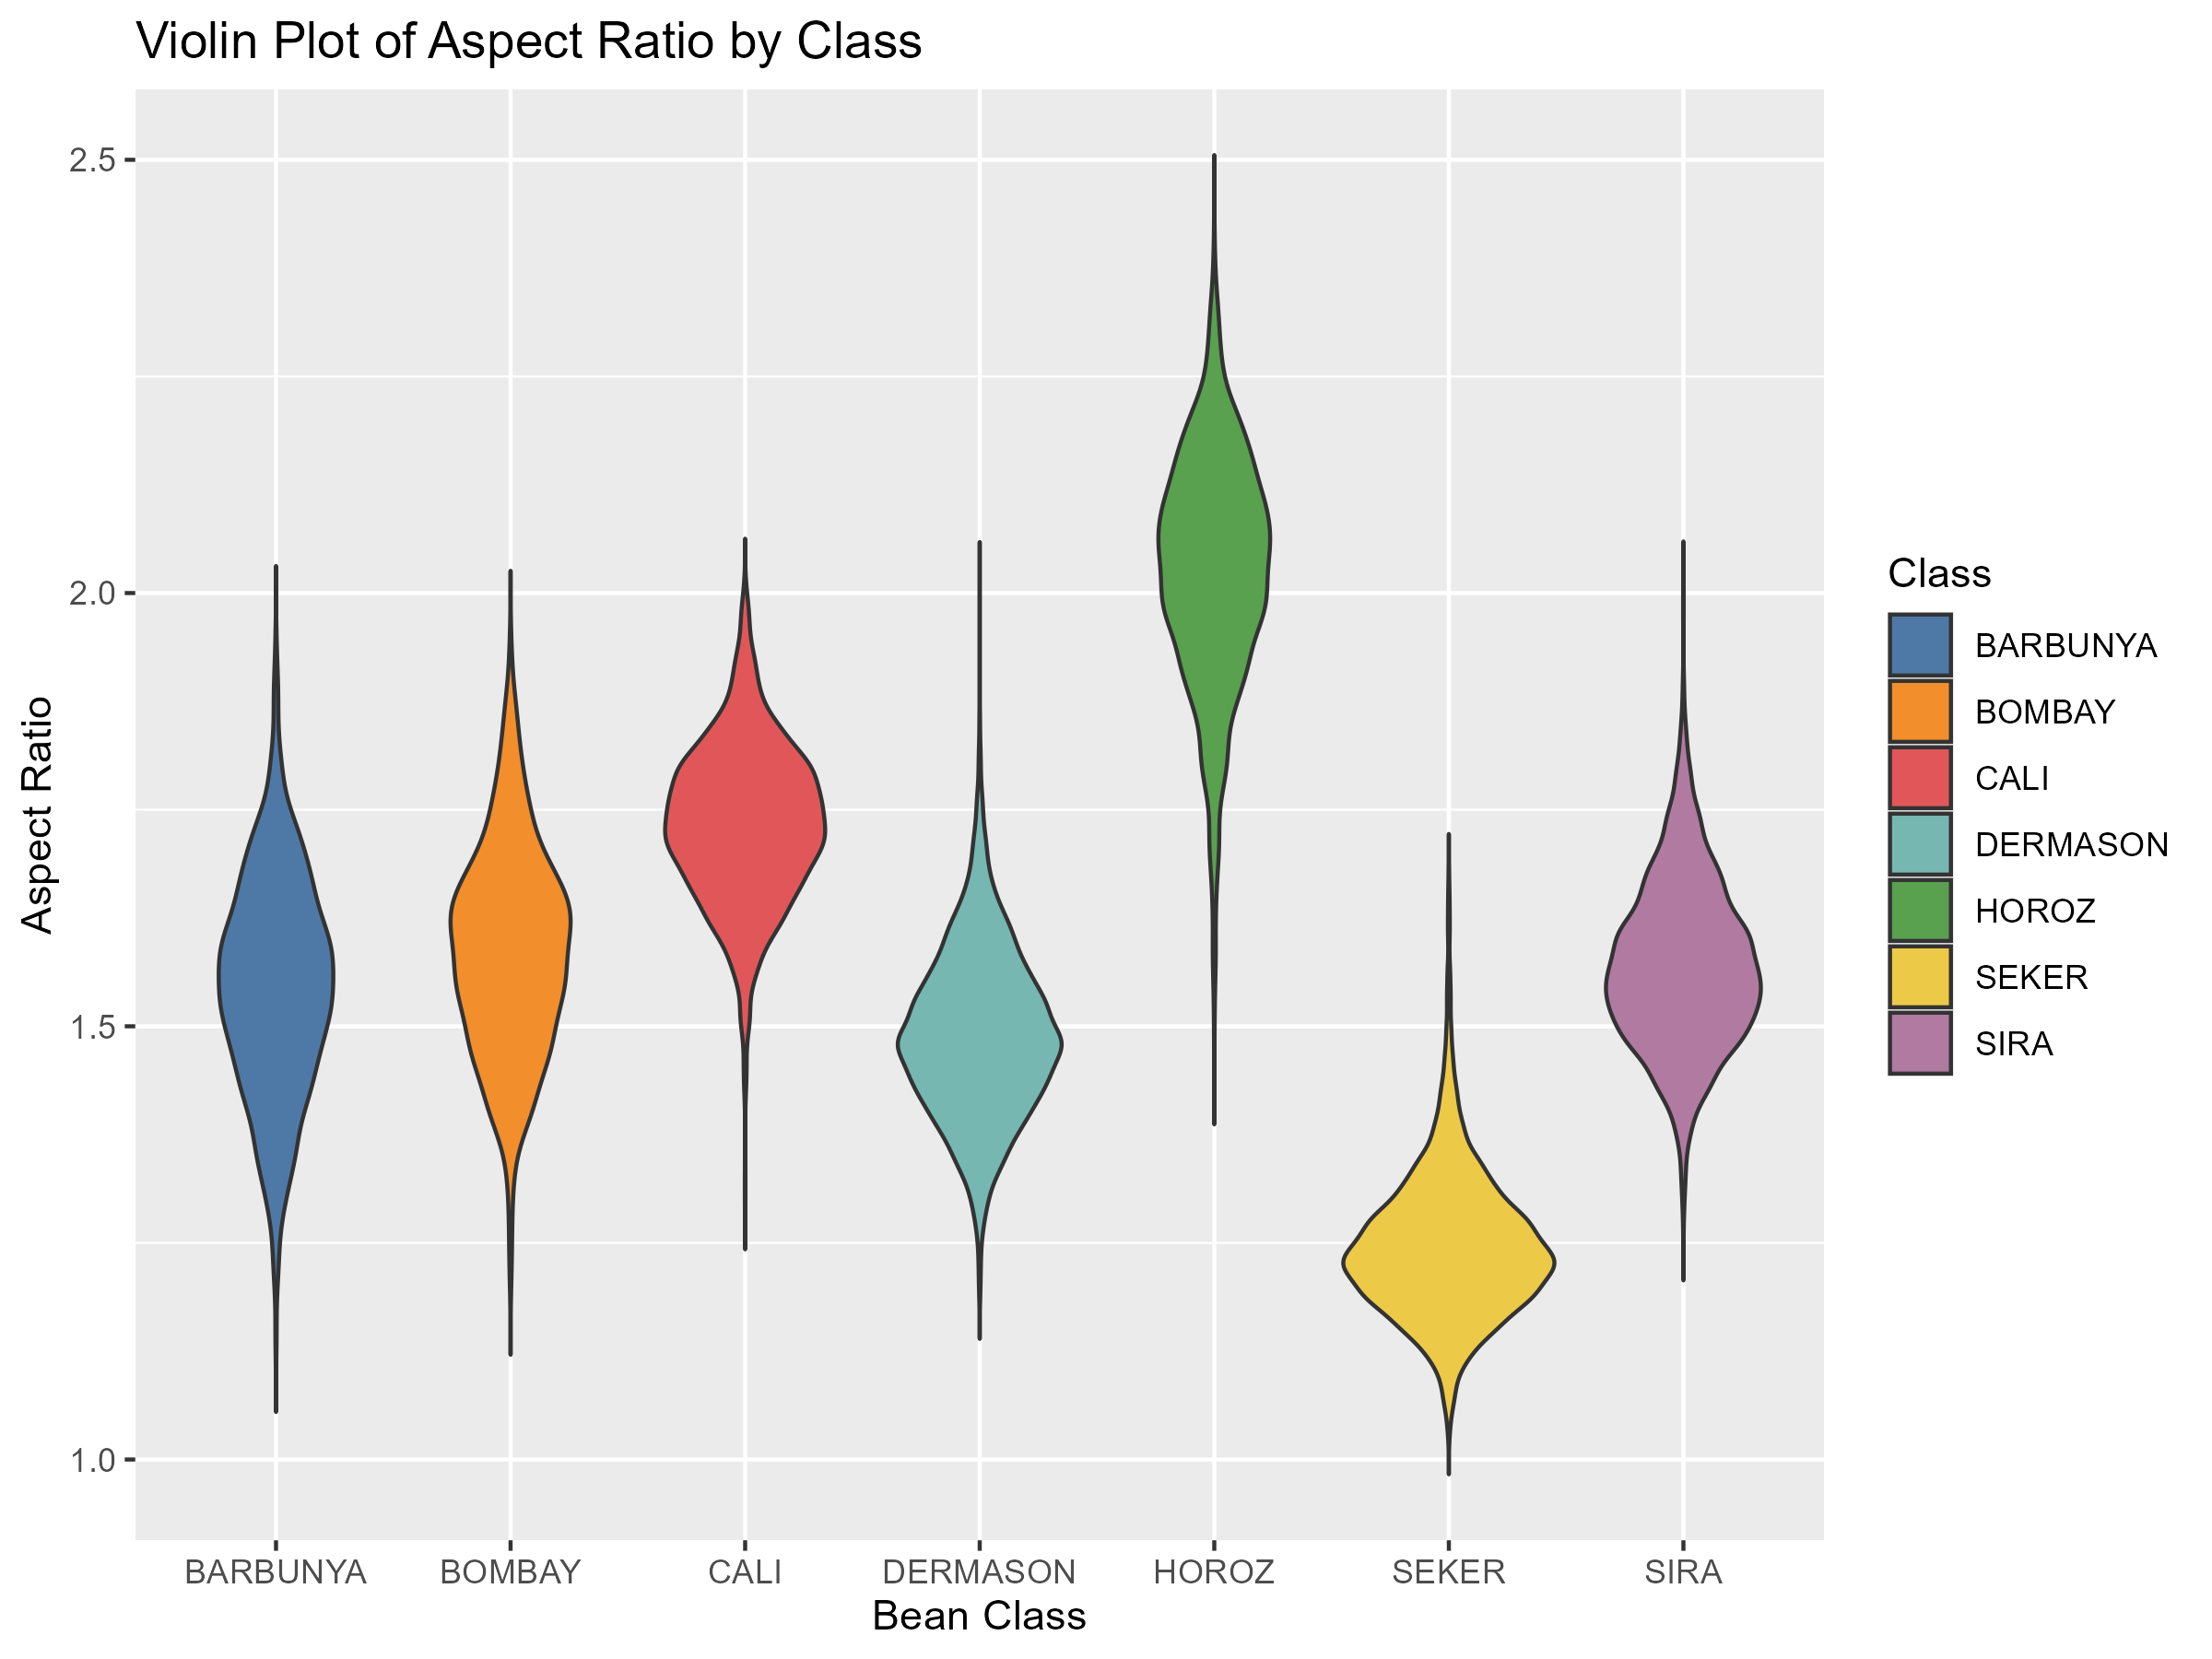
\includegraphics[width=0.8\textwidth]{graphs/violinplot_aspect_ratio.png}
    \caption{Violin Plot of Aspect Ratio by Bean Class}
    \label{fig:violin_aspect_ratio}
\end{figure}
This violin plot displays the distribution of the aspect ratio for different classes of dry beans. Each bean class (such as BARBUNYA, BOMBAY, CALI, etc.) is represented along the x-axis, and the aspect ratio of the beans is shown along the y-axis. The violin shapes illustrate the distribution of aspect ratio values within each bean class, with the width of the shape representing the density of data points at different aspect ratios. For instance, the HOROZ class shows a wider spread and a peak towards higher aspect ratios, indicating more variability. The plot allows for a visual comparison of the aspect ratios among different bean classes, highlighting variations in shape characteristics.


\newpage


\subsection{Histogram of Convex Area}
\noindent\textbf{Objective:} This histogram provides insights into the distribution of the \textit{Convex Area} of beans. It answers: "What are the common ranges for the convex area in the dataset?"

\noindent\textbf{Explanation:} The histogram reveals a right-skewed distribution, with most beans having a convex area concentrated in the lower range, while a few have significantly larger values.

\begin{figure}[H]
    \centering
    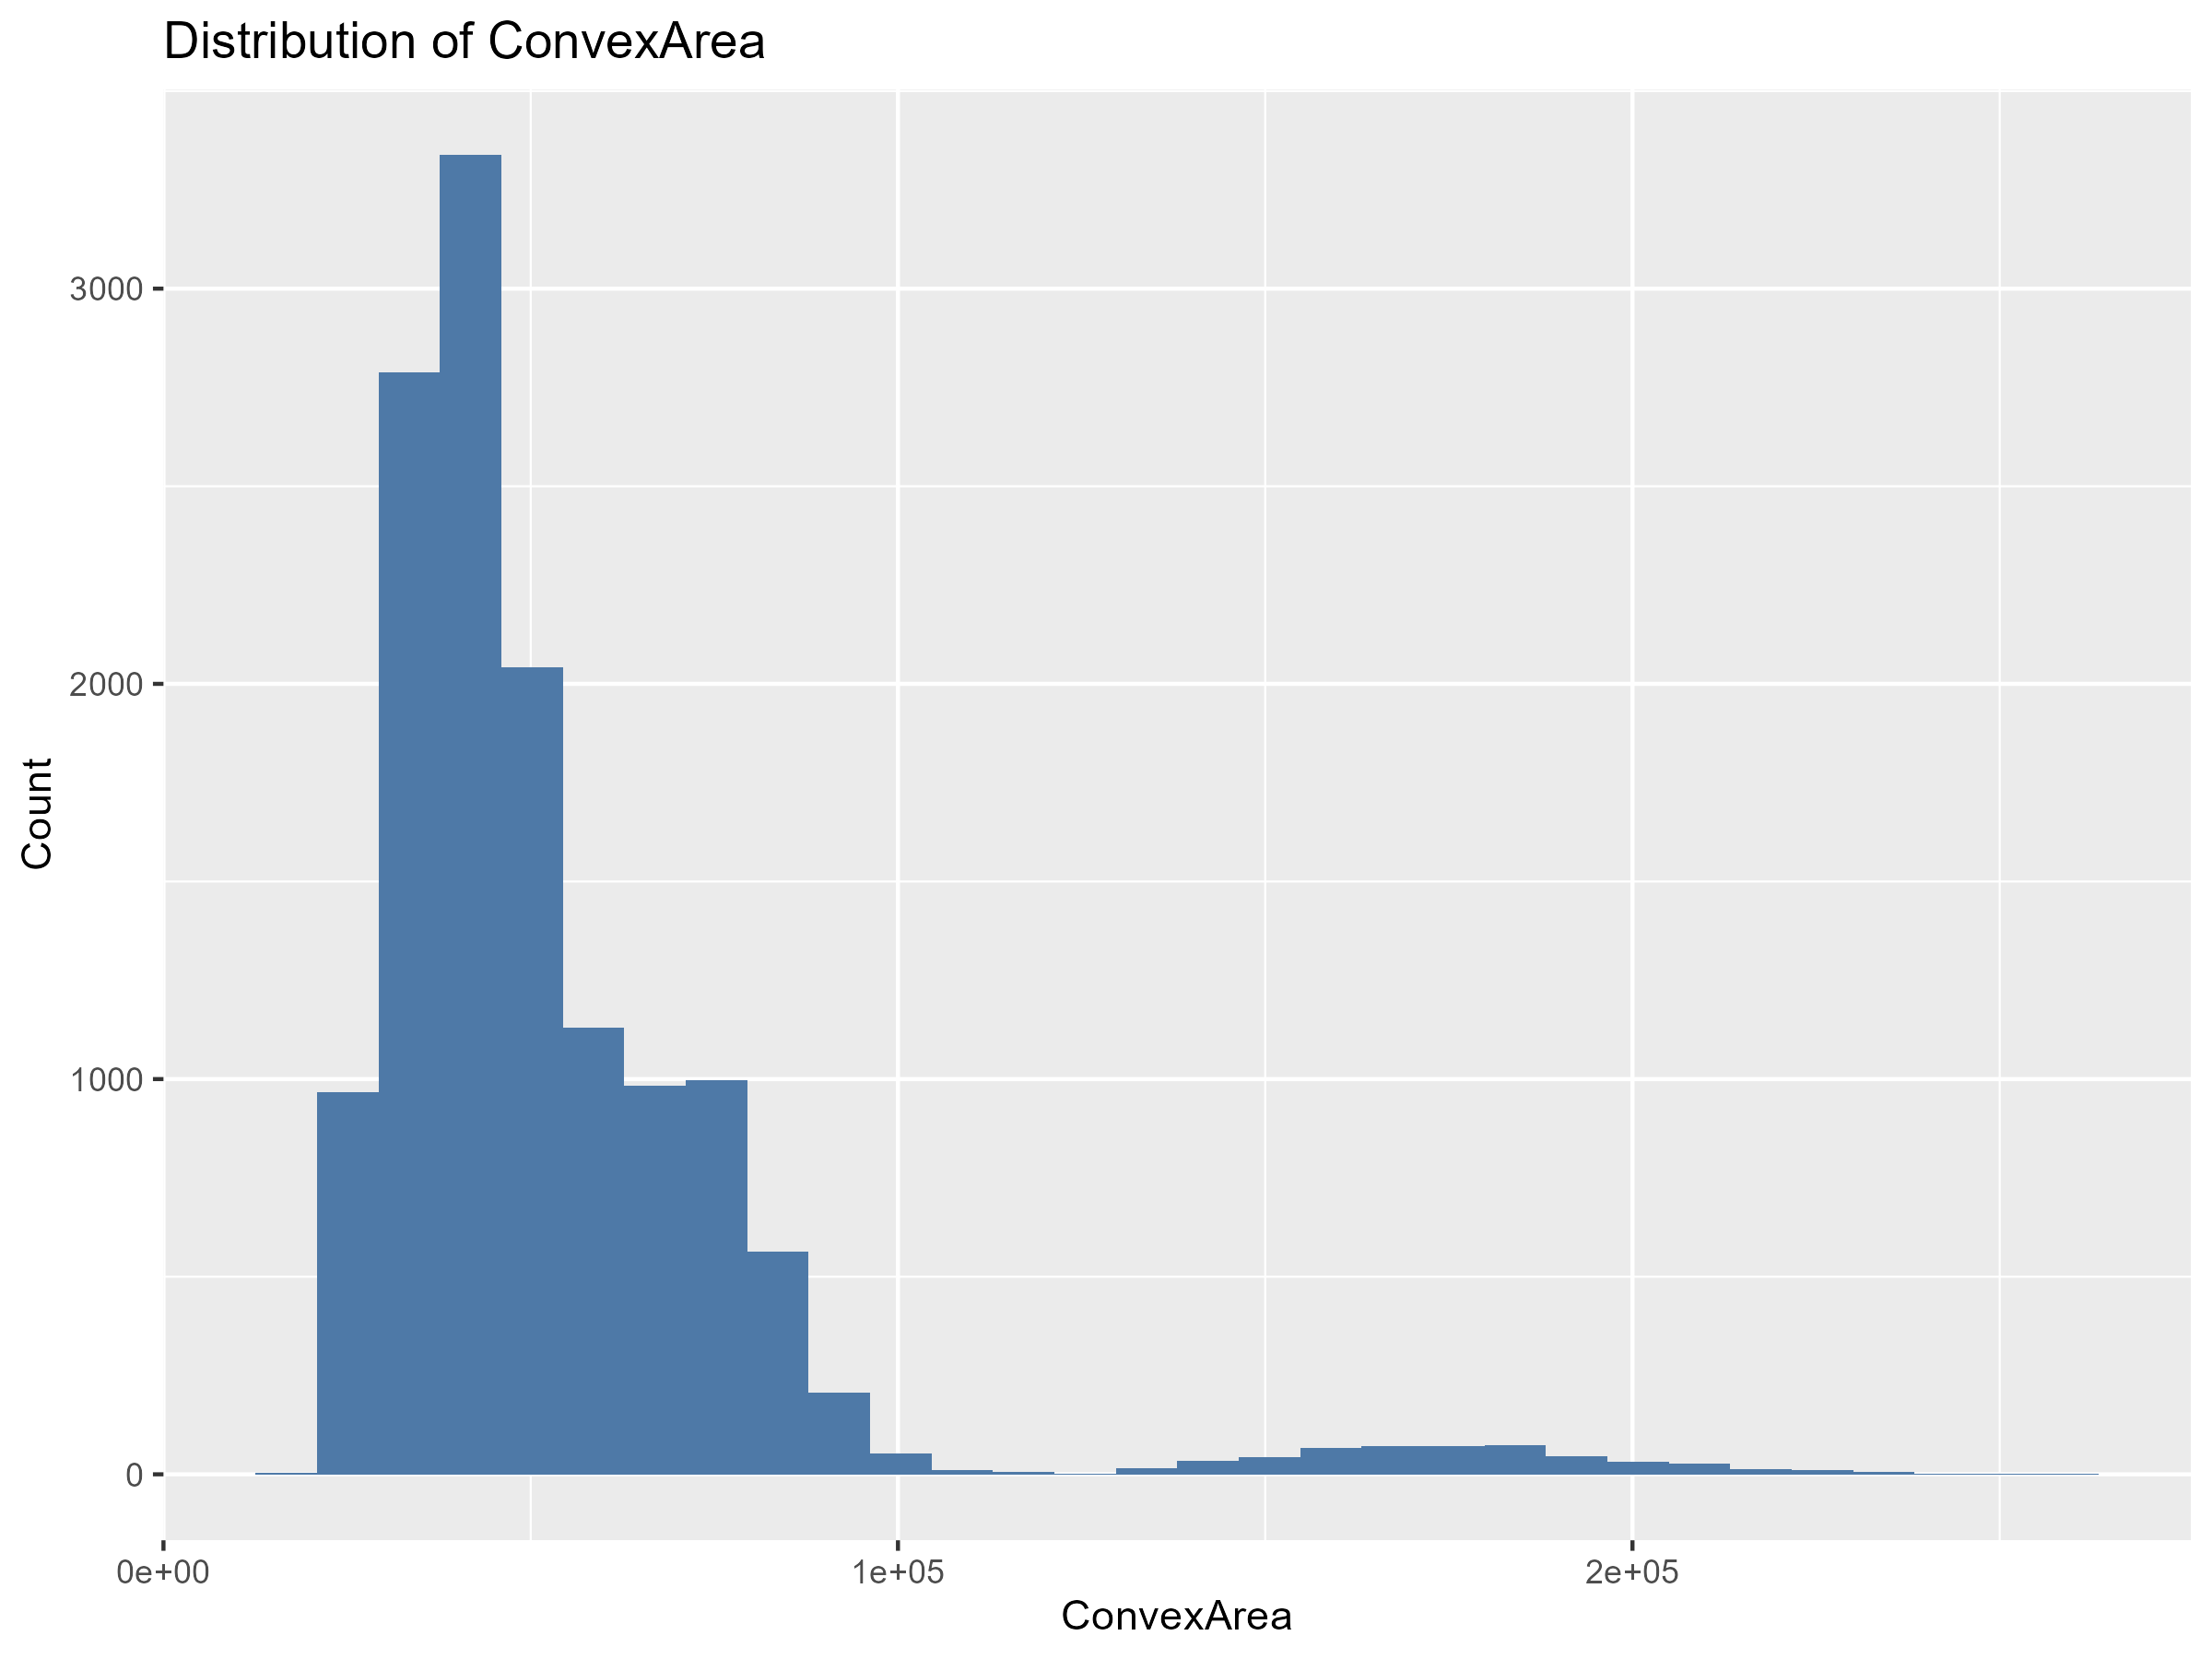
\includegraphics[width=0.8\textwidth]{graphs/histogram_convexarea.png}
    \caption{Histogram of Convex Area}
    \label{fig:histogram_convex_area}
\end{figure}
This histogram represents the distribution of the convex area of dry beans. The x-axis shows the convex area values, while the y-axis represents the count of beans that fall into each convex area range. The distribution is heavily right-skewed, with most beans having a convex area concentrated in the lower range, as indicated by the peak near the left side of the plot. The tail on the right shows a gradual decrease in frequency, implying that only a small number of beans have large convex areas. This plot provides an overview of the spread and frequency of convex area values, revealing significant skewness towards lower values.


\newpage


\subsection{Pairwise Plot of Key Features}
\noindent\textbf{Objective:} The pairwise plot visualizes relationships between multiple key features, addressing: "How do different features interact, and are there correlations that stand out?"

\noindent\textbf{Explanation:} The plot indicates strong correlations among features such as \textit{Area}, \textit{Perimeter}, and \textit{Axis Lengths}, which could impact feature selection and model training.

\begin{figure}[H]
    \centering
    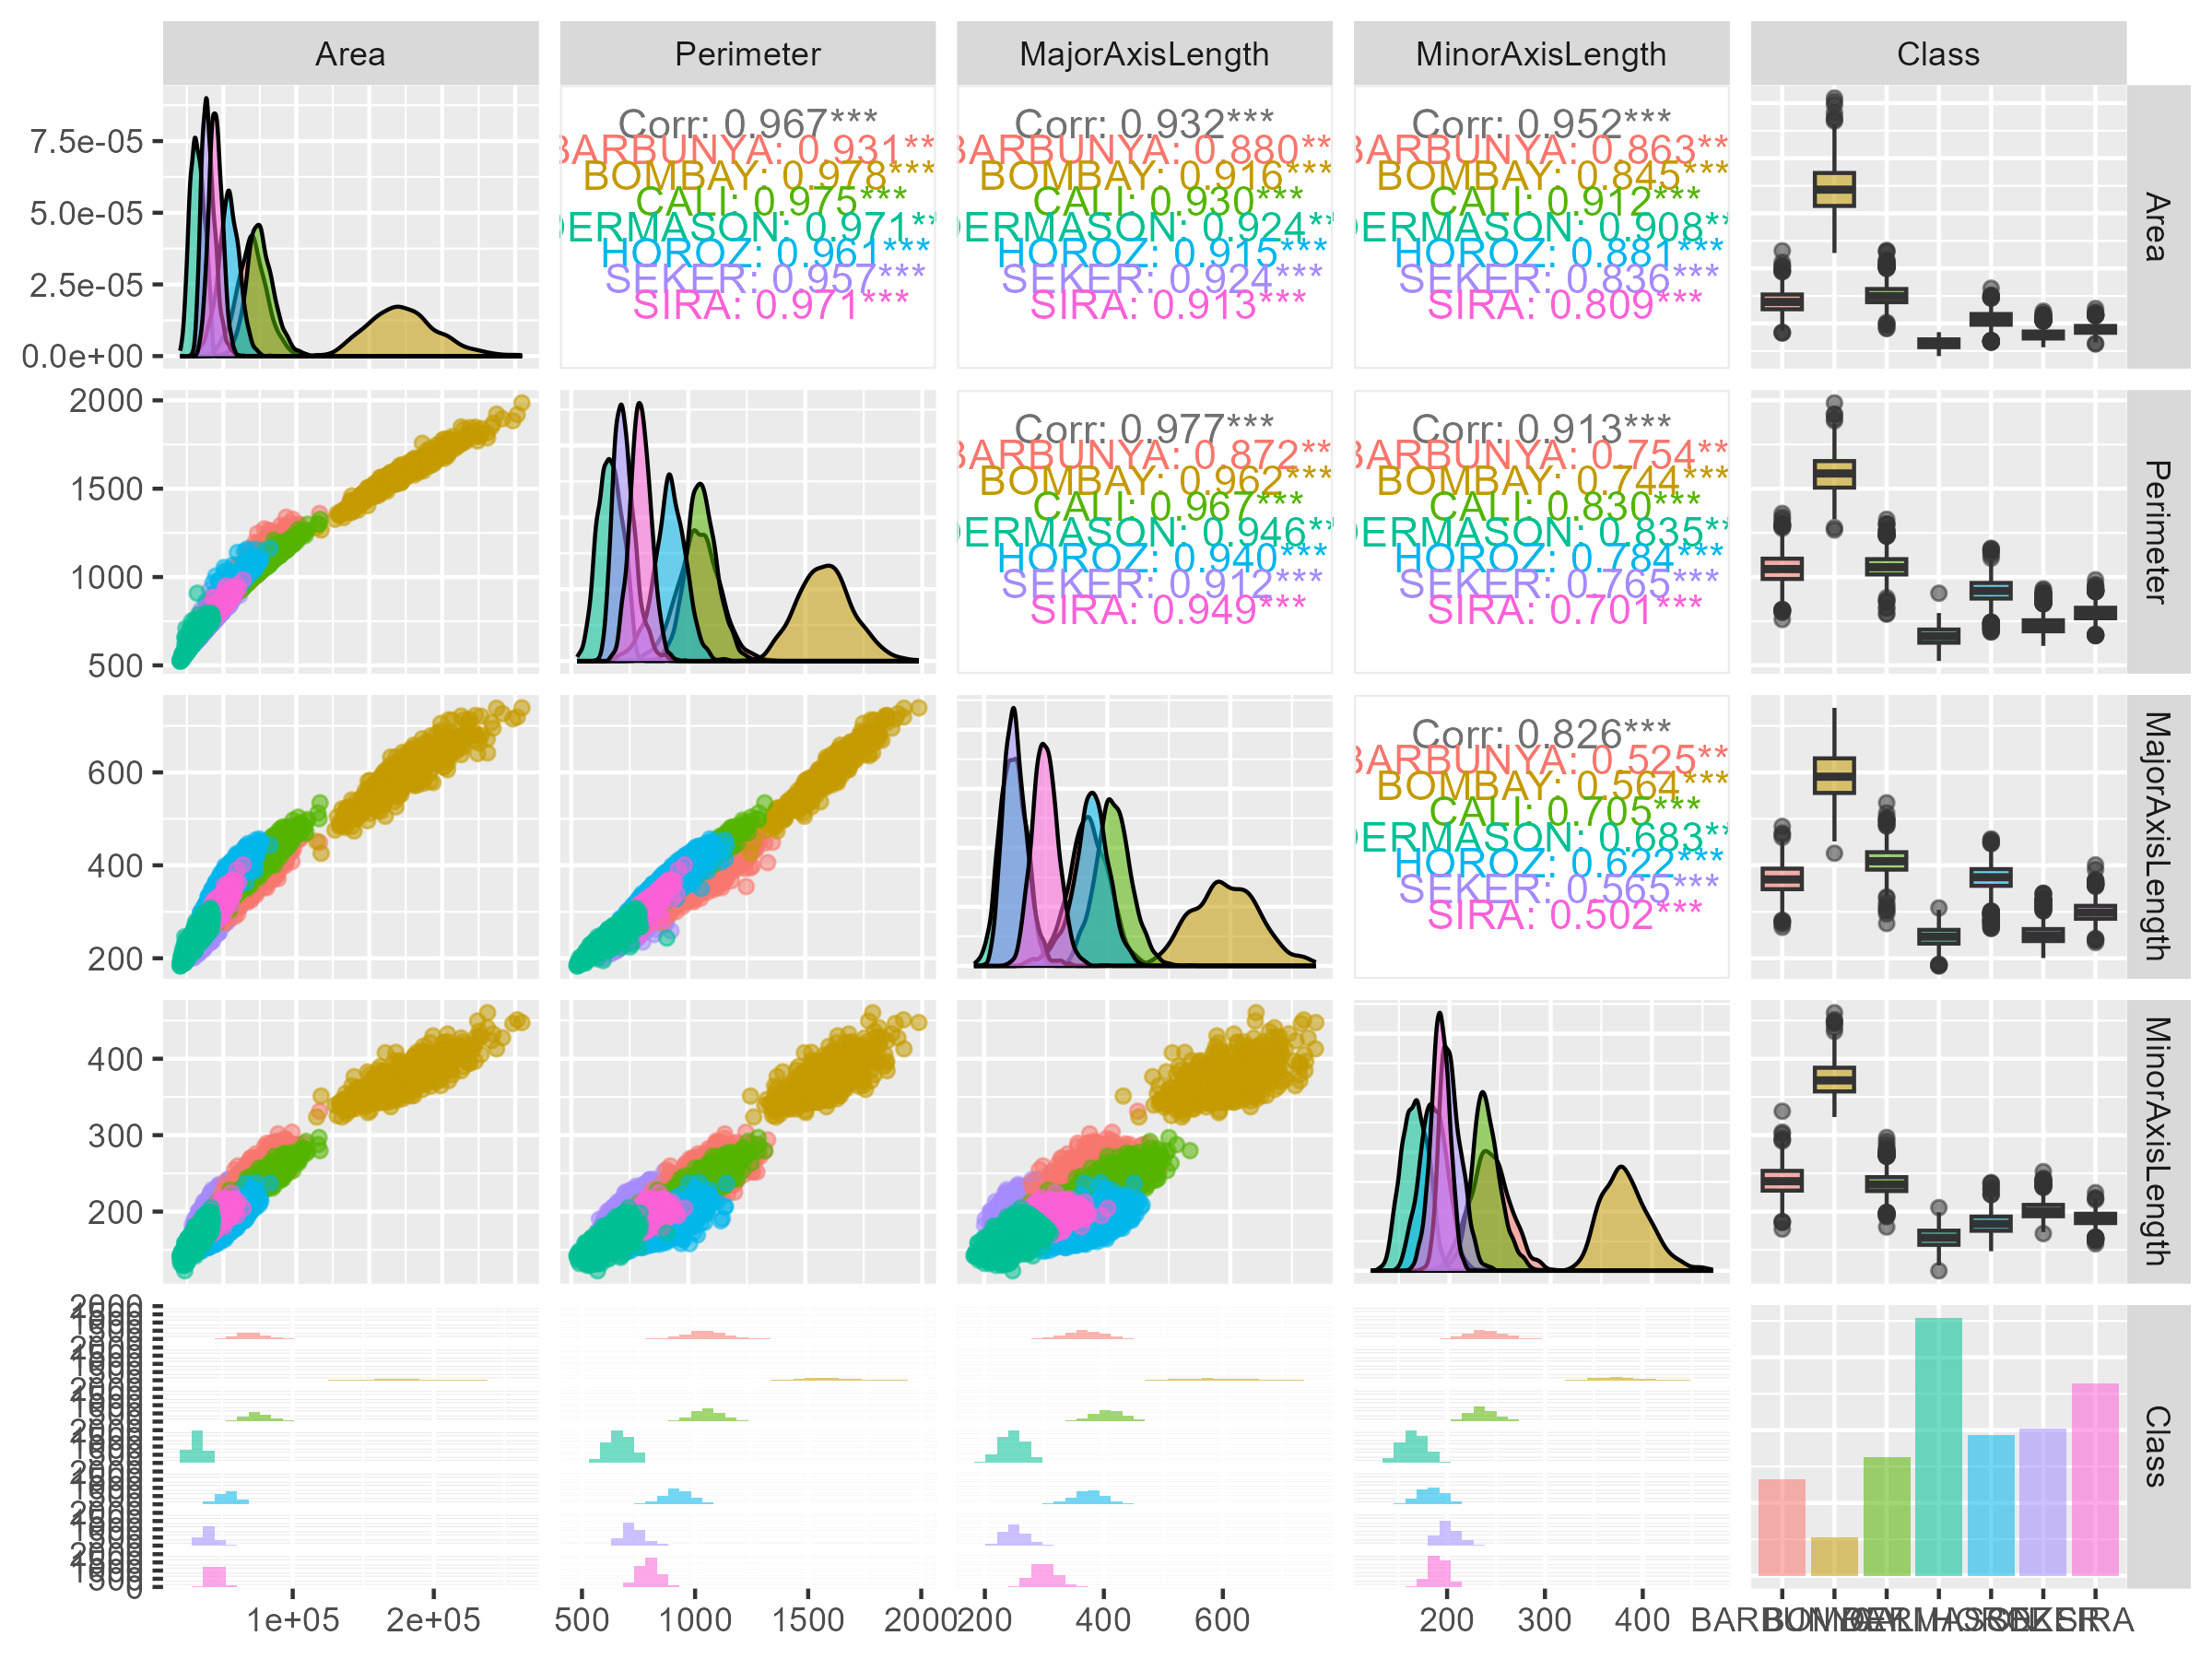
\includegraphics[width=0.8\textwidth]{graphs/pairwise_plot.png}
    \caption{Pairwise Plot of Key Features}
    \label{fig:pairwise_plot}
\end{figure}
The pairwise plot visualizes relationships between several key features, such as area, perimeter, compactness, and axis lengths. Each scatter plot represents the relationship between two features, while the diagonal shows the density of each feature. Strong correlations between area, perimeter, and axis lengths are evident, especially for larger beans like BOMBAY. This plot provides an overview of the dataset, helping identify important features for classification models.


\newpage


\subsection{Density Plot of Solidity by Bean Class}
\noindent\textbf{Objective:} This plot shows the variation in \textit{Solidity} across different bean classes, answering: "Do certain classes show higher solidity, indicating a more compact shape?"

\noindent\textbf{Explanation:} The density curves indicate that most bean classes, such as BARBUNYA and SEKER, have high \textit{Solidity} values, suggesting that they tend to be more compact in shape.

\begin{figure}[H]
    \centering
    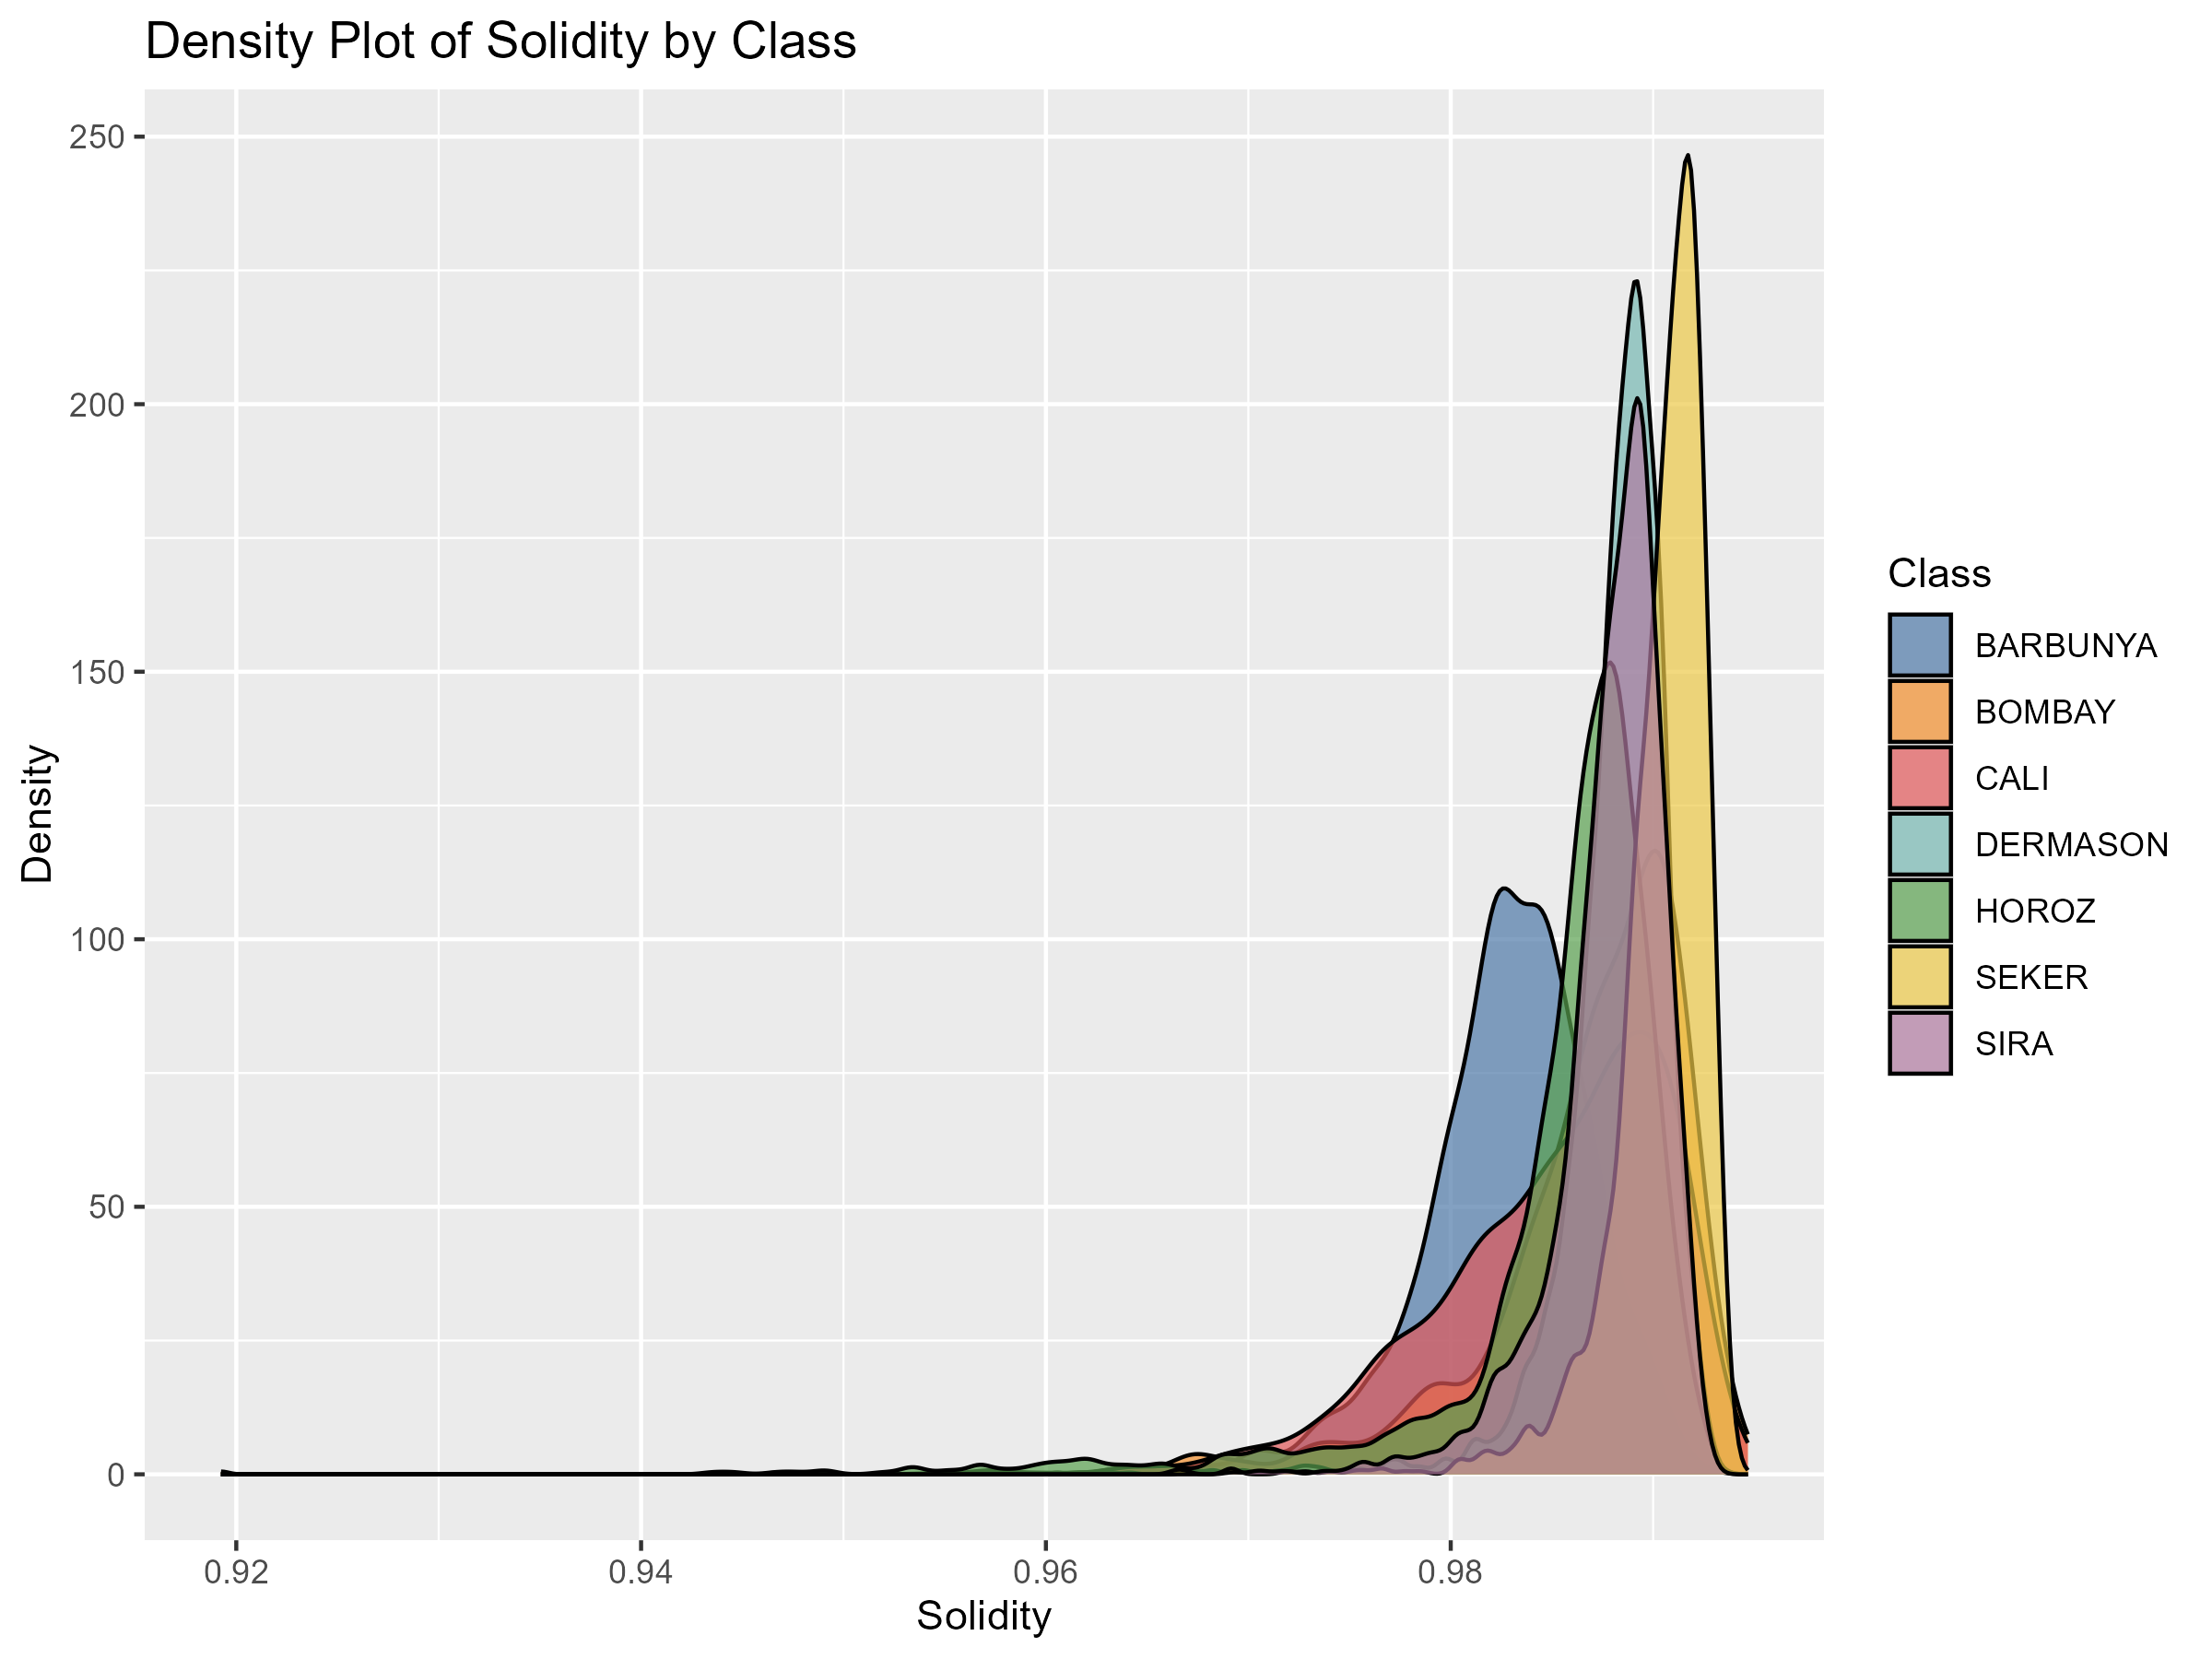
\includegraphics[width=0.8\textwidth]{graphs/density_solidity.png}
    \caption{Density Plot of Solidity by Bean Class}
    \label{fig:density_solidity}
\end{figure}
This density plot visualizes the distribution of Solidity across different bean classes. The x-axis represents solidity values, while the y-axis shows the density of data points for each class. Most bean classes, such as BARBUNYA and SEKER, have high solidity values clustering around 0.99, indicating strong solidity for most instances. Classes like BOMBAY have lower solidity values with a broader spread. The plot highlights that most classes are tightly clustered with high solidity, while a few, such as BOMBAY, have slightly lower values.

\newpage

\subsection{Scatter Plot of ShapeFactor3 vs ShapeFactor4}
\noindent\textbf{Objective:} This scatter plot visualizes the relationship between \textit{ShapeFactor3} and \textit{ShapeFactor4} for different bean classes, answering: "How are these shape factors related?"

\noindent\textbf{Explanation:} The plot reveals clustering patterns where certain classes exhibit higher values for both shape factors, indicating a possible relationship that may help differentiate bean types.

\begin{figure}[H]
    \centering
    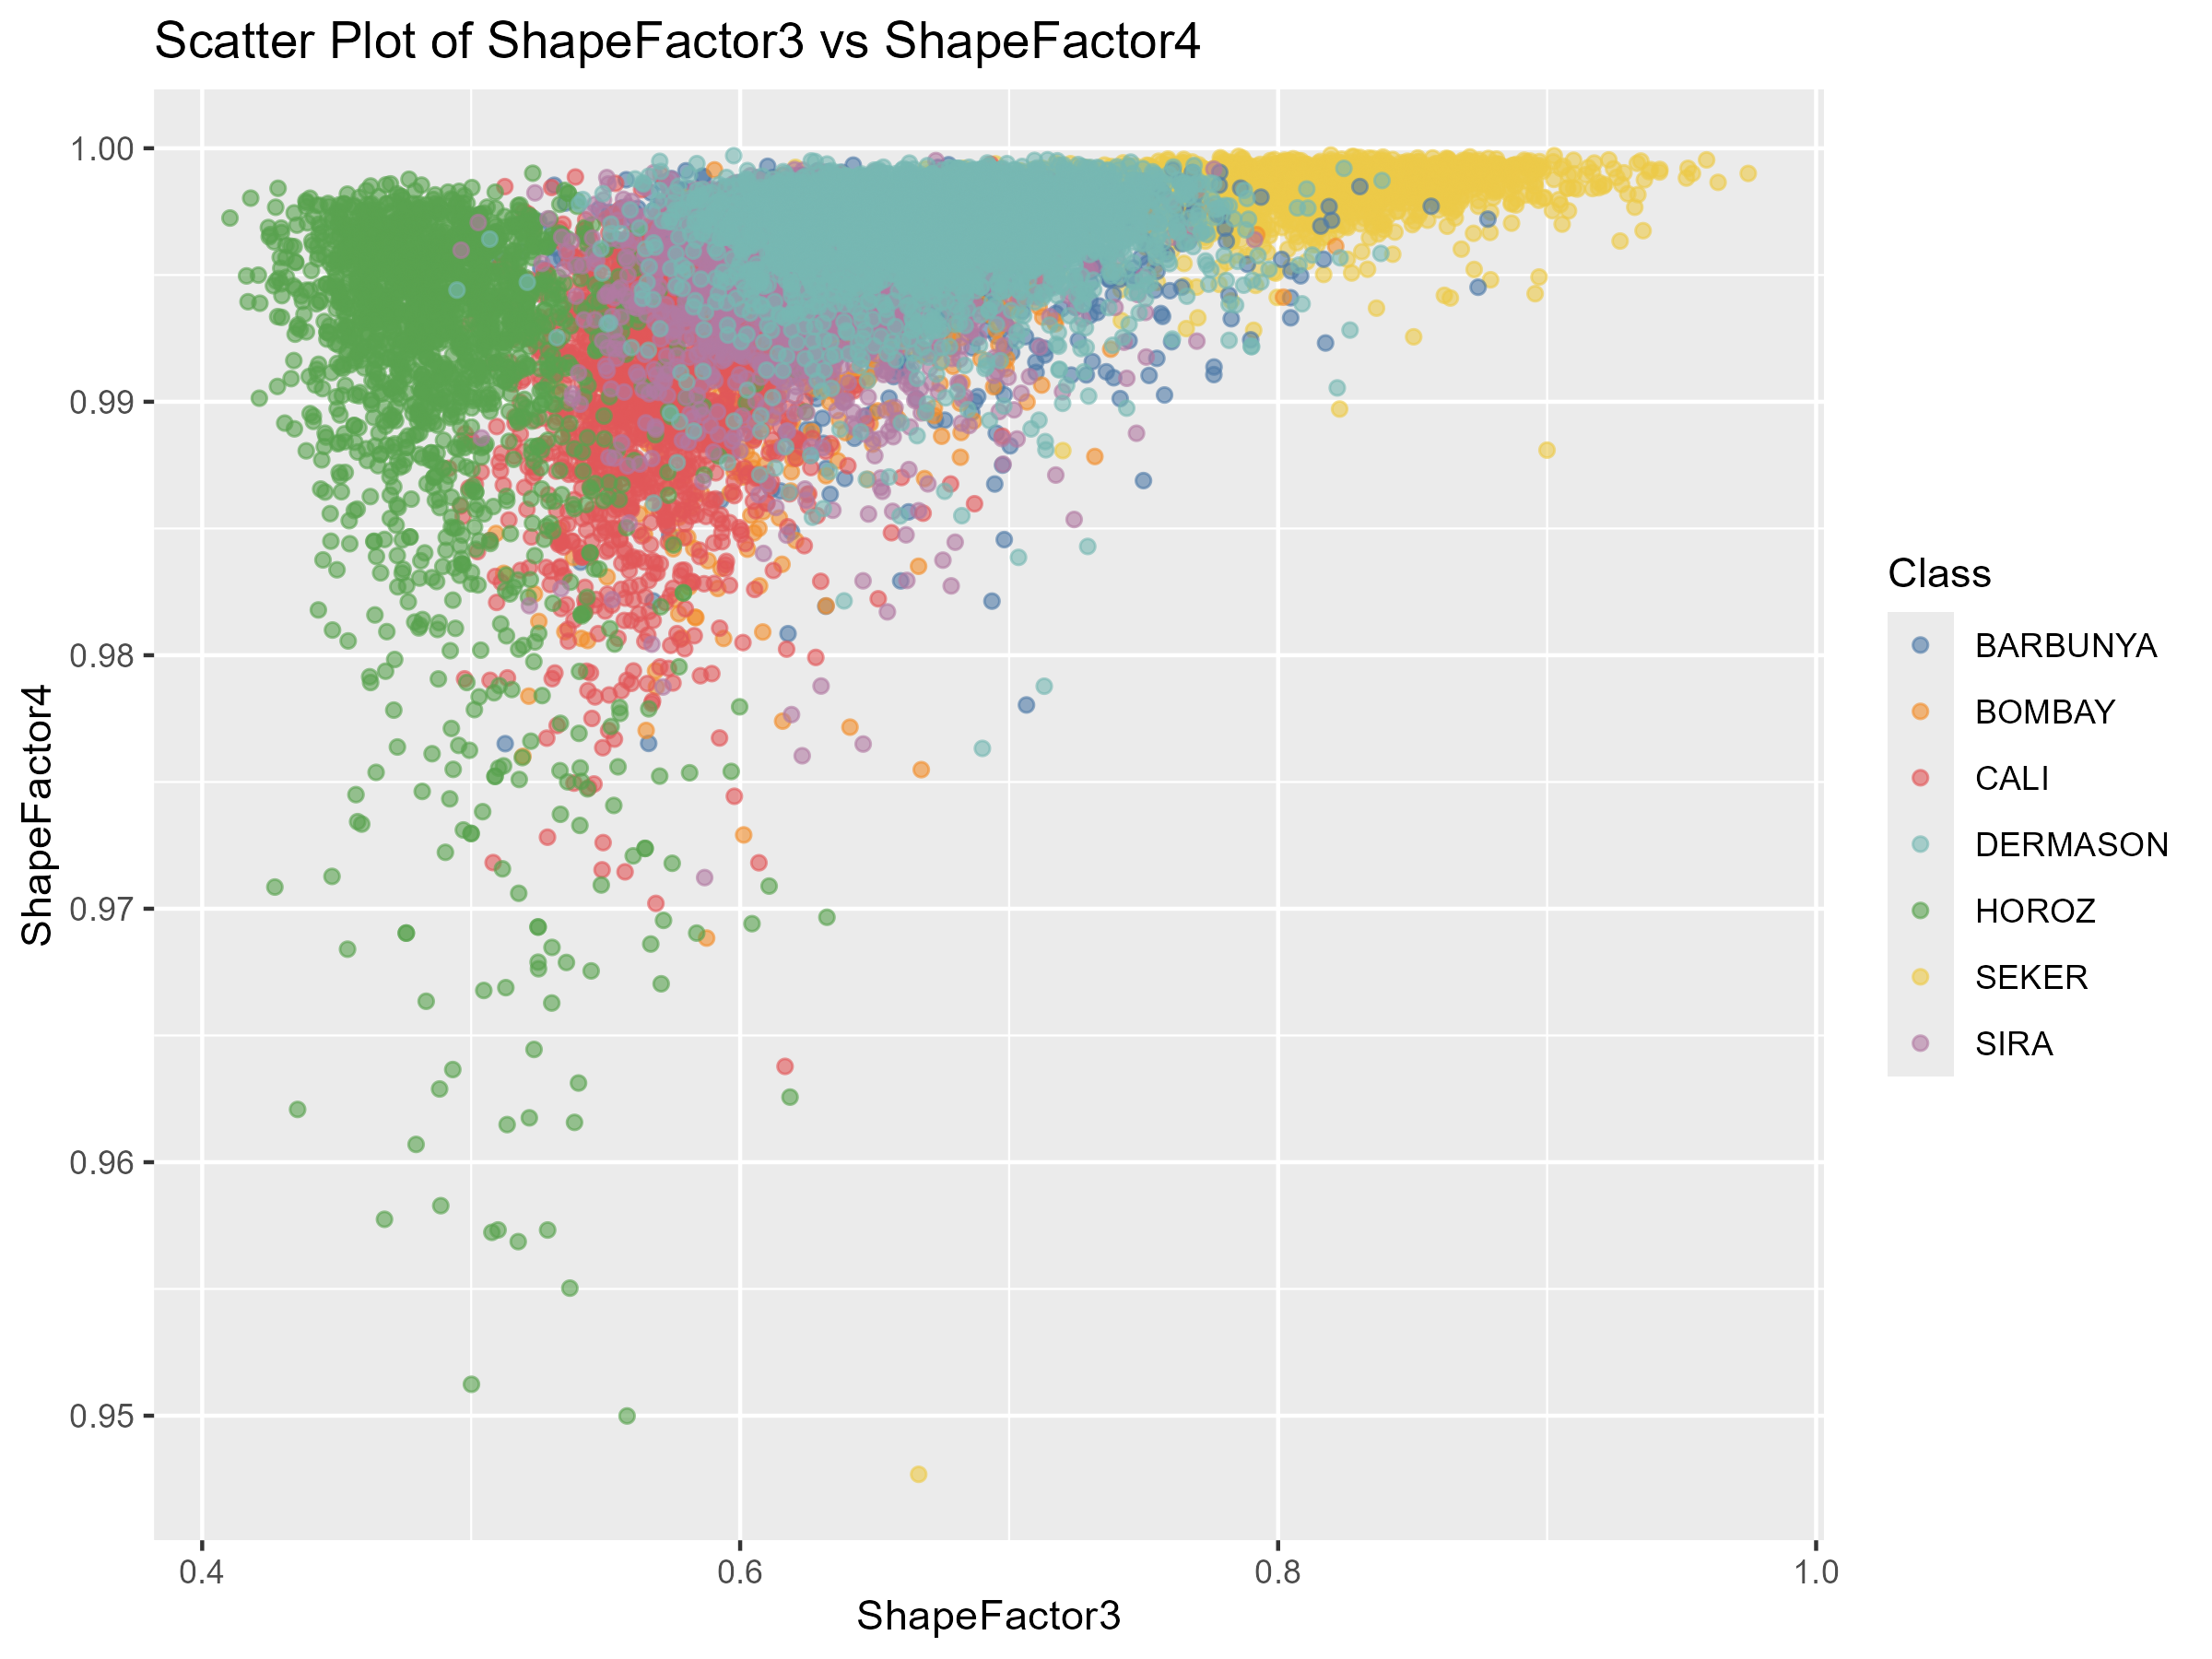
\includegraphics[width=0.8\textwidth]{graphs/scatter_shapefactor3_shapefactor4.png}
    \caption{Scatter Plot of ShapeFactor3 vs ShapeFactor4}
    \label{fig:scatter_shape3_shape4}
\end{figure}
This scatter plot shows the relationship between ShapeFactor3 and ShapeFactor4 for different bean classes. The x-axis represents ShapeFactor3, while the y-axis represents ShapeFactor4, with points color-coded by bean class. Most data points cluster around higher ShapeFactor4 values (close to 1.0), while ShapeFactor3 varies from 0.5 to 0.9. SEKER beans (yellow) tend to have the highest ShapeFactor3 values, while HOROZ (green) has a broader spread across lower values. 

\newpage

\subsection{Boxplot of ShapeFactor1 by Bean Class}
\noindent\textbf{Objective:} This boxplot compares the distribution of \textit{ShapeFactor1} across different bean classes, addressing: "How does ShapeFactor1 vary between classes?"

\noindent\textbf{Explanation:} The plot shows that classes such as HOROZ and DERMASON have higher median \textit{ShapeFactor1} values compared to other classes, indicating variations in shape characteristics.

\begin{figure}[H]
    \centering
    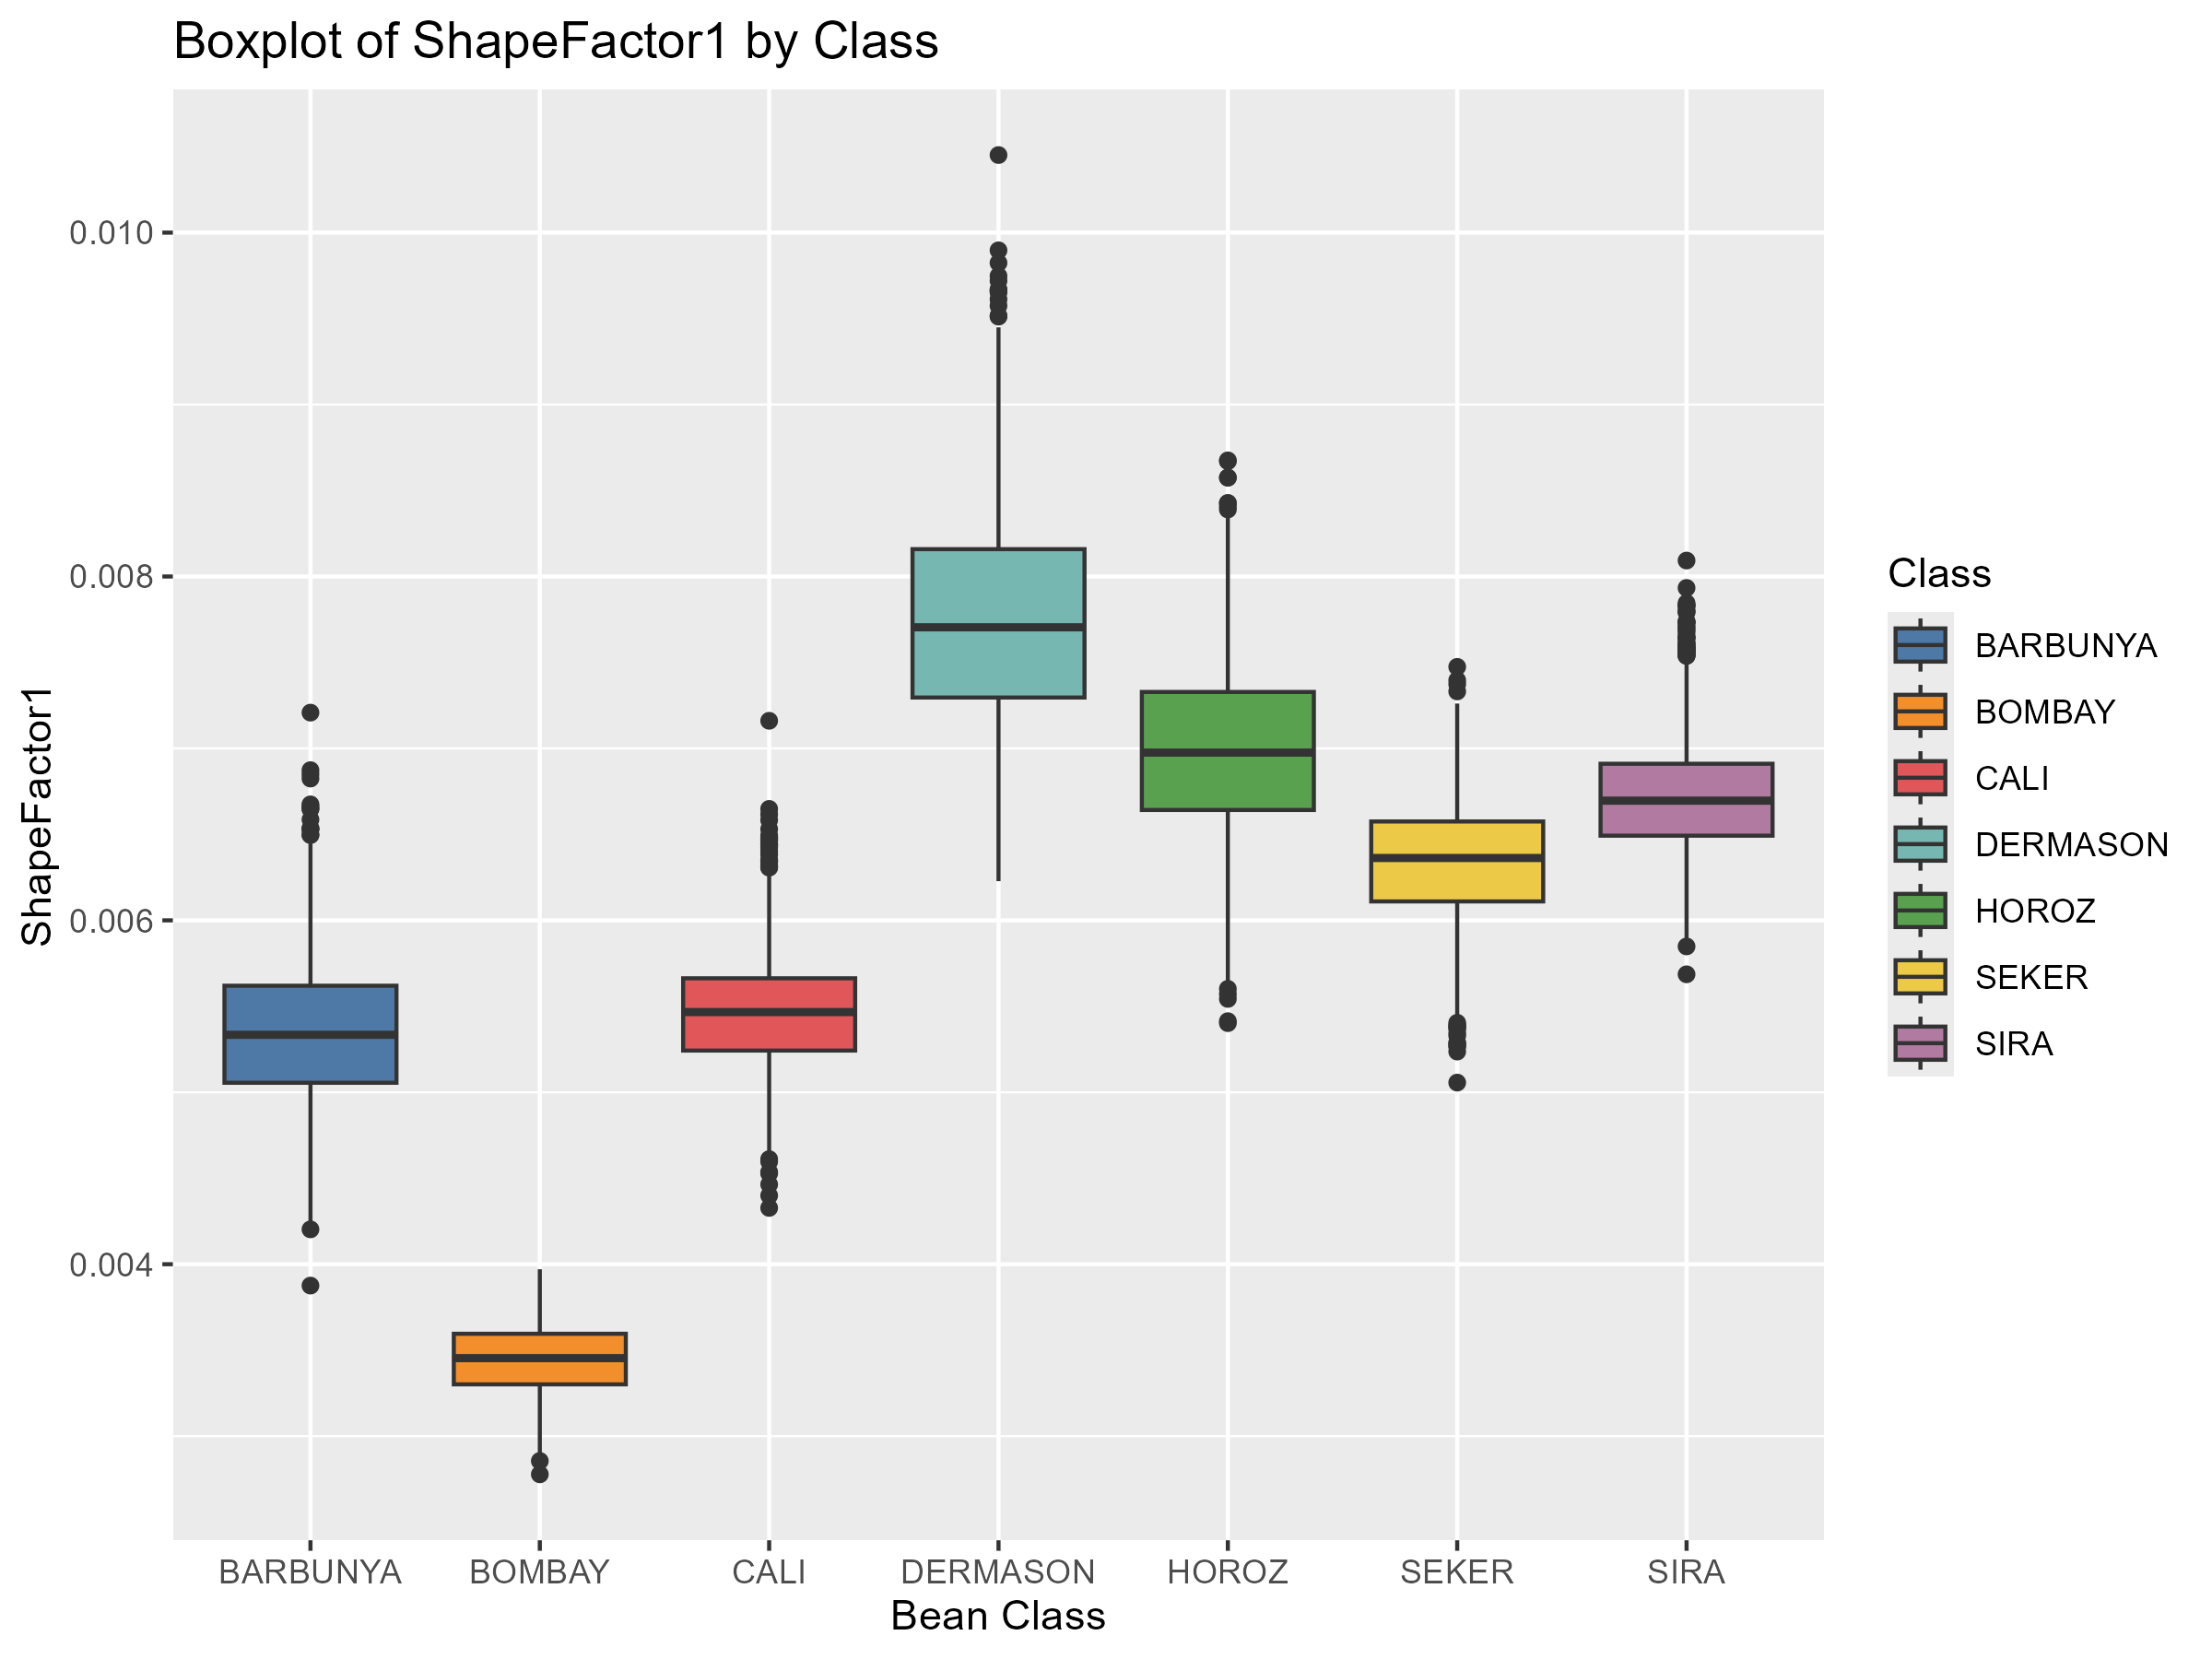
\includegraphics[width=0.8\textwidth]{graphs/boxplot_shapefactor1.png}
    \caption{Boxplot of ShapeFactor1 by Bean Class}
    \label{fig:boxplot_shapefactor1}
\end{figure}
This boxplot visualizes the distribution of ShapeFactor1 across different bean classes. The x-axis represents the bean classes, and the y-axis shows the values for ShapeFactor1. Each box represents the interquartile range (IQR) with the median marked inside, while the whiskers extend to show the range of the data. DERMASON and HOROZ have higher median values for ShapeFactor1, while BOMBAY has the lowest median. Outliers, shown as dots, are observed in classes like SIRA and DERMASON, indicating beans with unusual ShapeFactor1 values.

\newpage

\subsection{Histogram of ShapeFactor2}
\noindent\textbf{Objective:} This histogram illustrates the distribution of \textit{ShapeFactor2} values across the dataset, answering: "What are the common ranges for ShapeFactor2?"

\noindent\textbf{Explanation:} The histogram shows that most beans have ShapeFactor2 values concentrated in certain ranges, with some classes displaying distinct peaks. This indicates variability in shape characteristics among different bean types.

\begin{figure}[H]
    \centering
    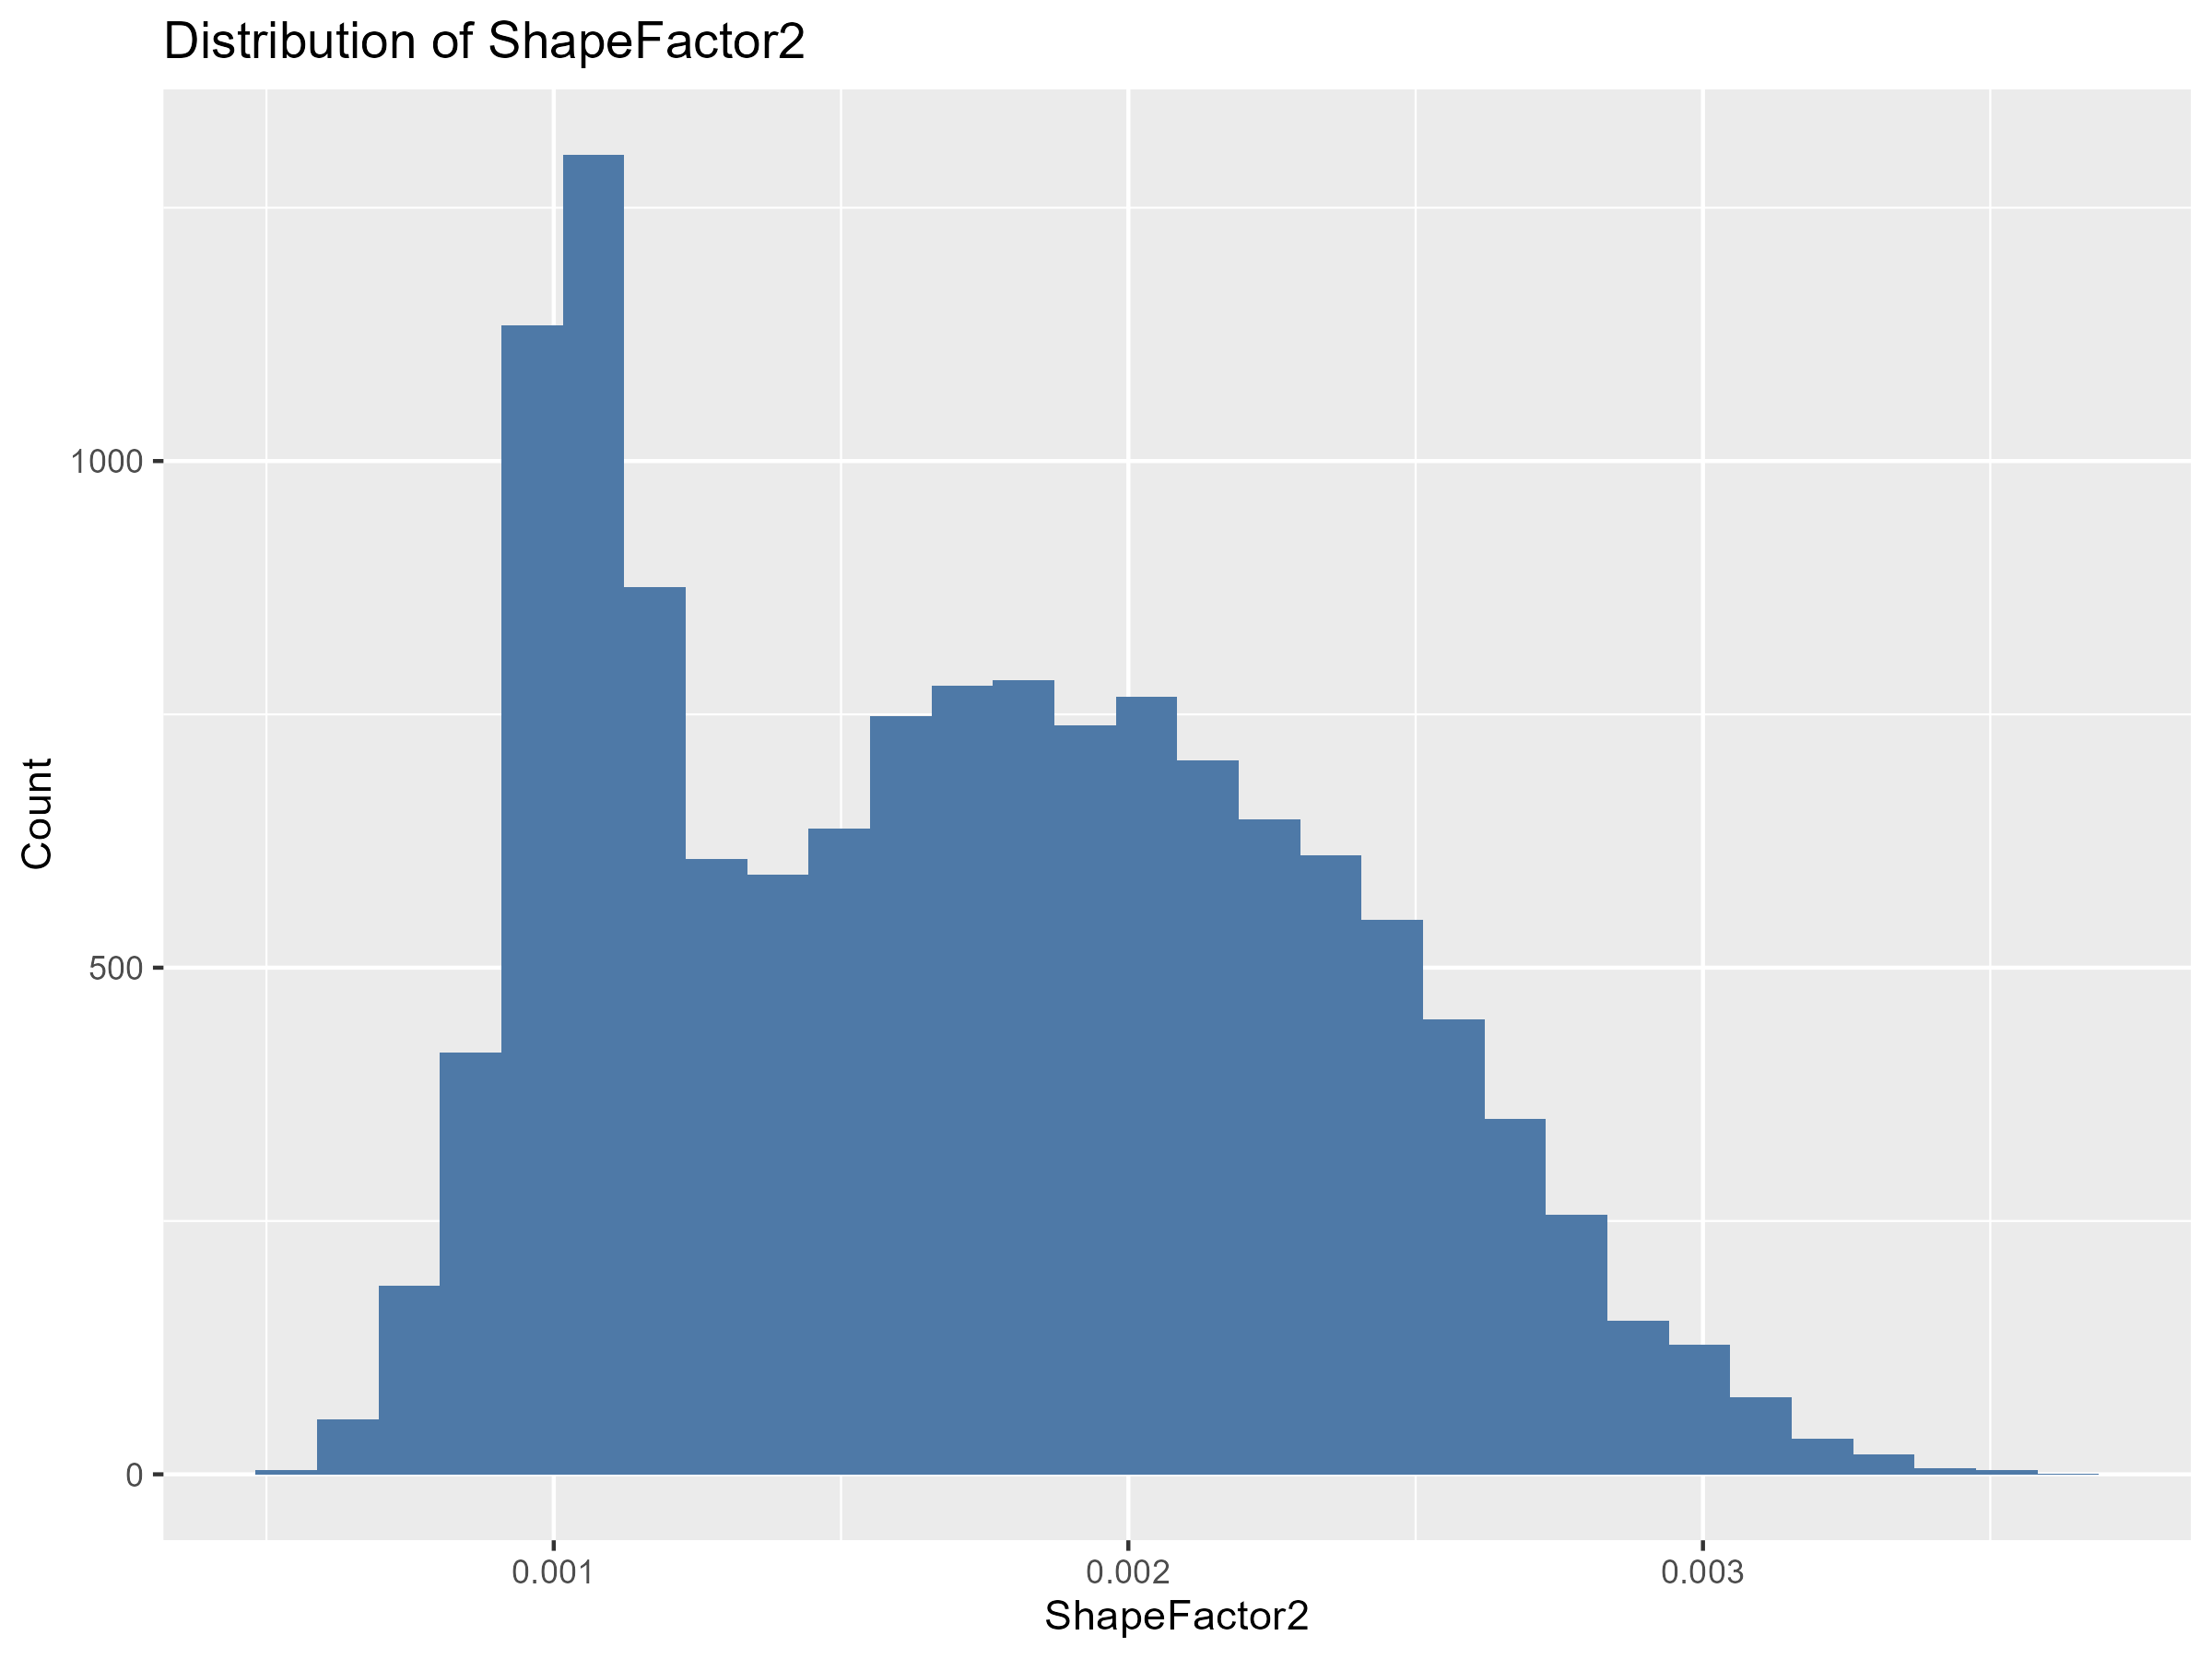
\includegraphics[width=0.8\textwidth]{graphs/histogram_shapefactor2.png}
    \caption{Histogram of ShapeFactor2}
    \label{fig:histogram_shapefactor2}
\end{figure}
This histogram illustrates the distribution of ShapeFactor2 in the dataset. The x-axis represents the values of ShapeFactor2, while the y-axis shows the count of instances for each value range. The distribution is slightly skewed to the right, with the highest count occurring around 0.001. The frequency decreases as ShapeFactor2 increases beyond this point, with fewer instances having values above 0.002. 

\newpage

\subsection{Density Plot of ShapeFactor3 by Bean Class}
\noindent\textbf{Objective:} This density plot illustrates the distribution of \textit{ShapeFactor3} across different bean classes, answering: "How does ShapeFactor3 vary among the different bean types?"

\noindent\textbf{Explanation:} The density plot reveals that some bean classes have distinct peaks at certain ShapeFactor3 values, while others show broader distributions. This variation can help identify shape characteristics that differentiate the bean classes.

\begin{figure}[H]
    \centering
    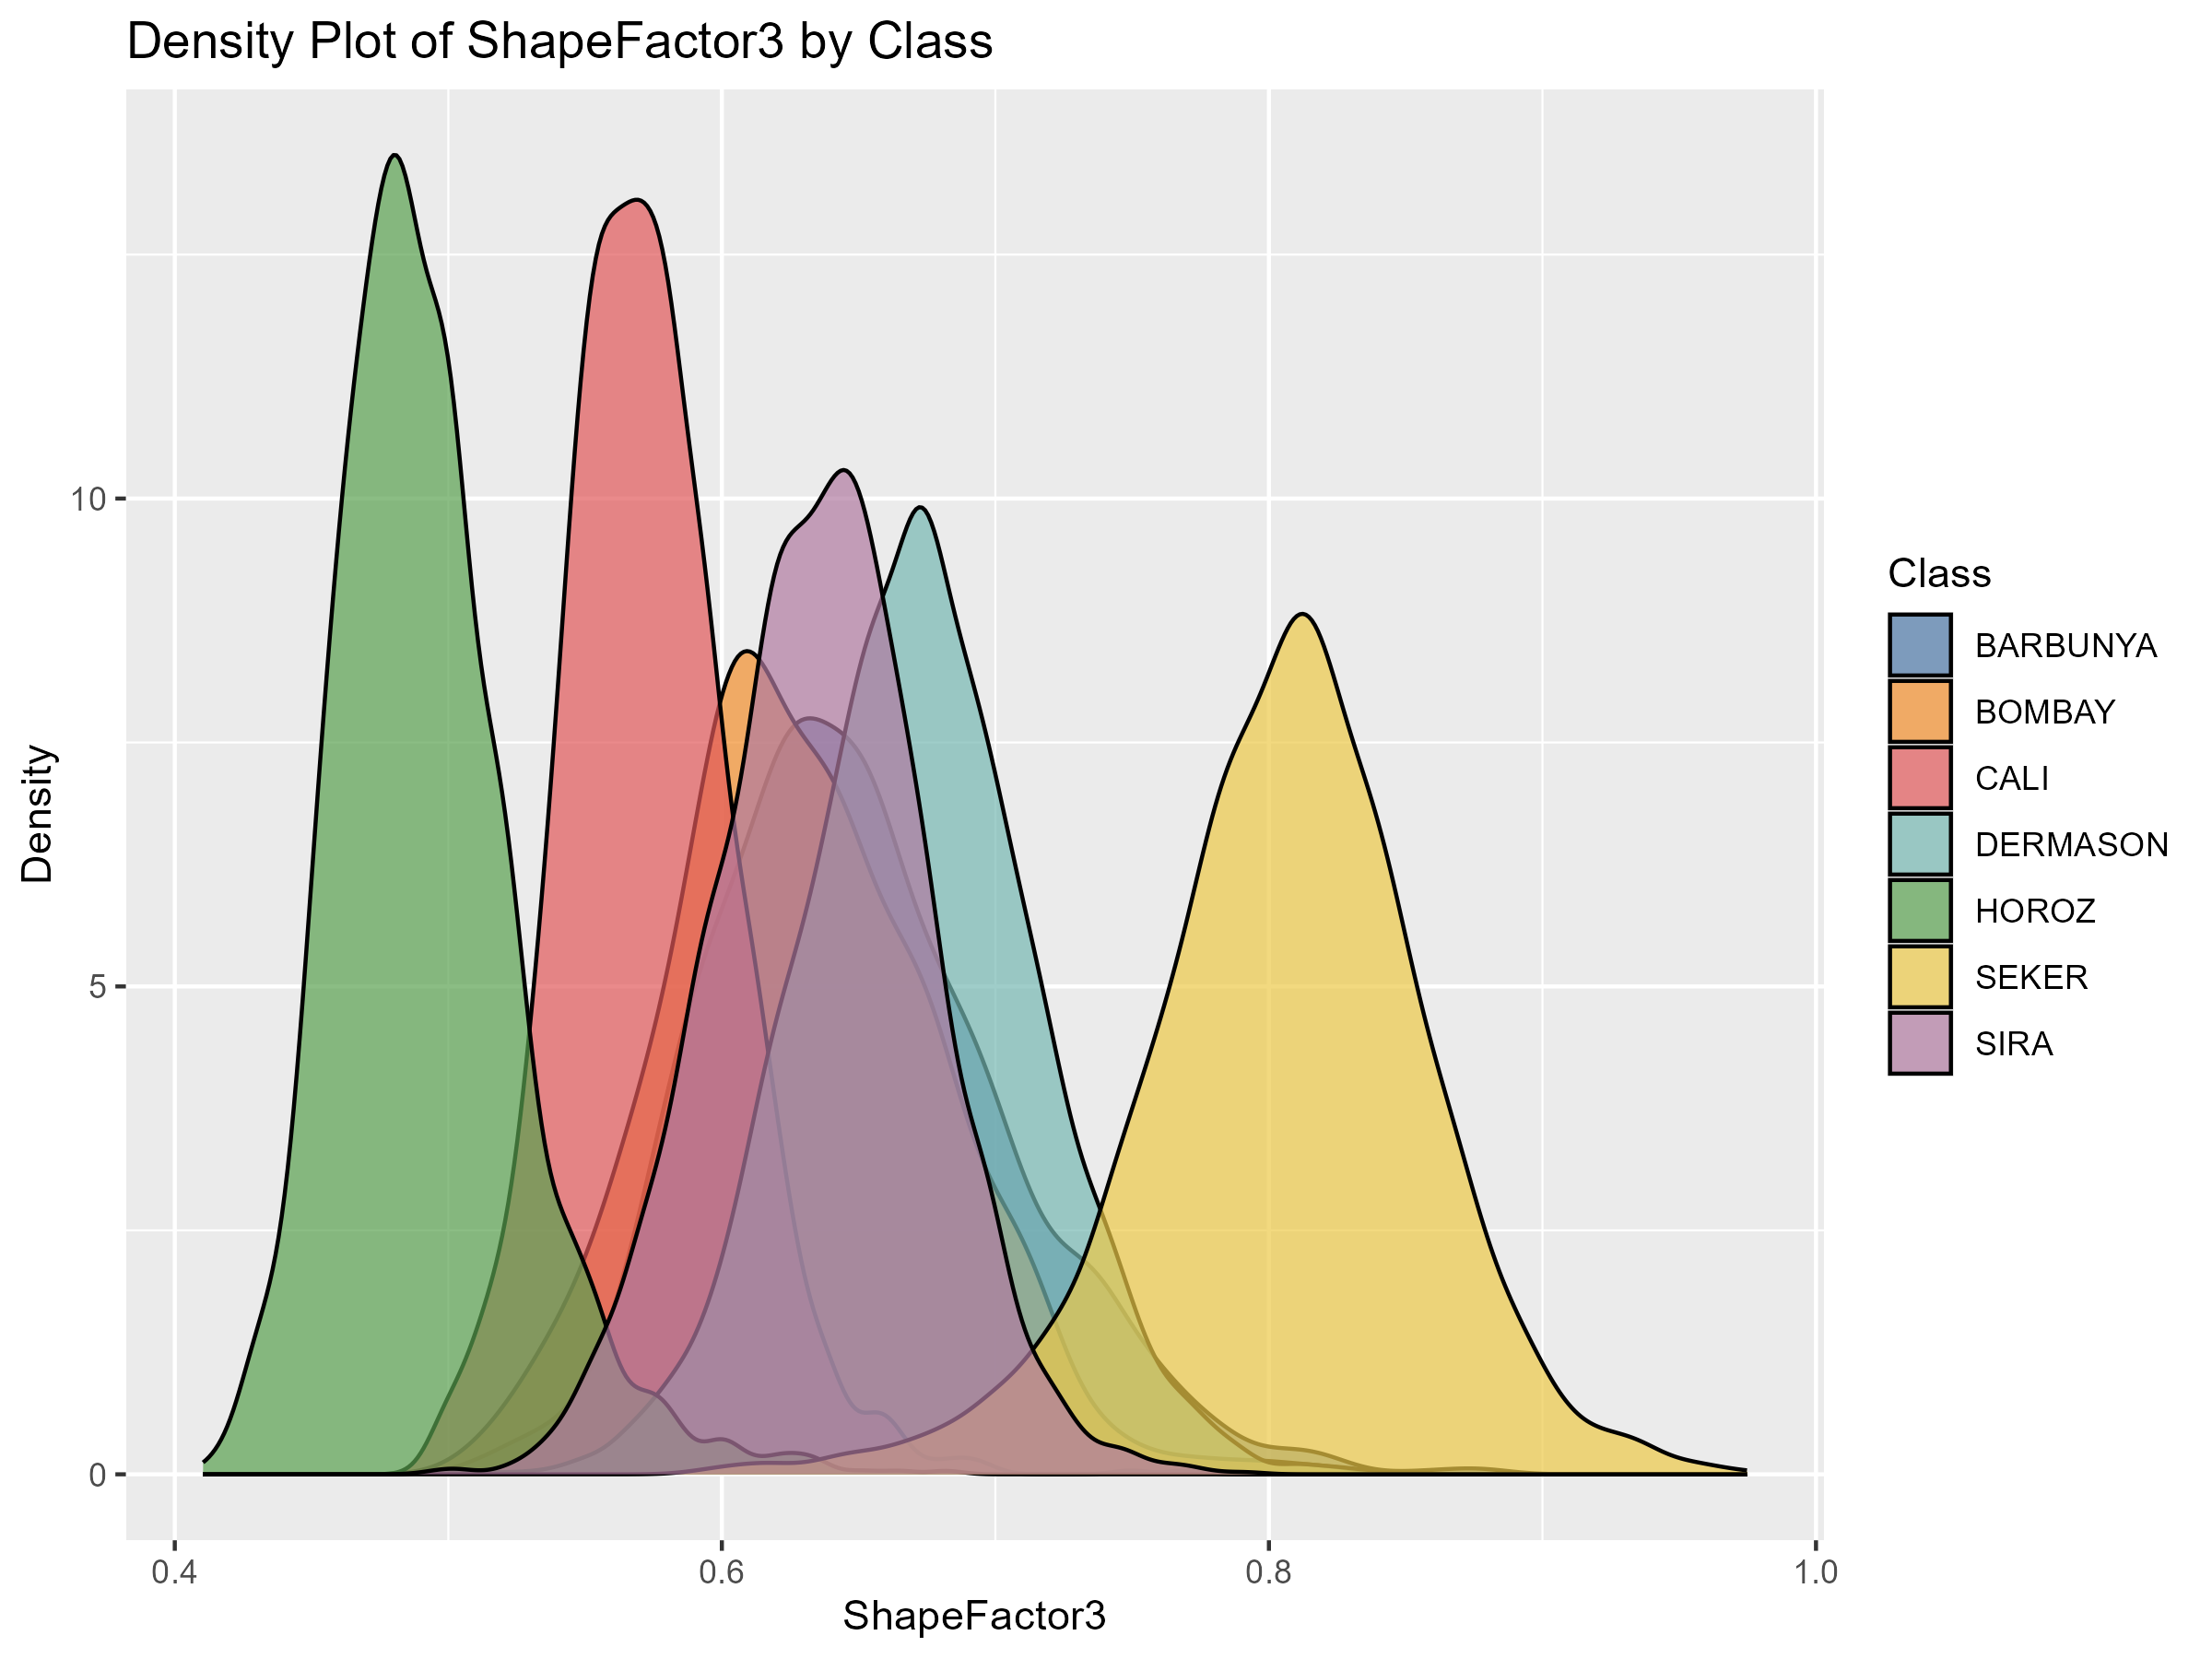
\includegraphics[width=0.8\textwidth]{graphs/density_shapefactor3.png}
    \caption{Density Plot of ShapeFactor3 by Bean Class}
    \label{fig:density_shapefactor3}
\end{figure}
This density plot shows the distribution of ShapeFactor3 for each bean class. The x-axis represents the values of ShapeFactor3, and the y-axis indicates the density of the data. HOROZ has the lowest ShapeFactor3 values, peaking around 0.5, while SEKER has the highest, peaking near 0.8. Classes like CALI and SIRA have overlapping distributions between 0.6 and 0.7. This plot helps compare how ShapeFactor3 values are distributed across the different bean classes, highlighting both similarities and differences.

\newpage

\subsection{Scatter Plot of EquivDiameter vs Solidity}
\noindent\textbf{Objective:} This scatter plot examines the relationship between \textit{EquivDiameter} and \textit{Solidity} across different bean classes, answering: "How are EquivDiameter and Solidity related among the bean types?"

\noindent\textbf{Explanation:} The plot shows that most bean classes cluster within specific ranges for EquivDiameter and Solidity. Beans with larger equivalent diameters tend to have varying levels of solidity, indicating differences in shape compactness across classes.

\begin{figure}[H]
    \centering
    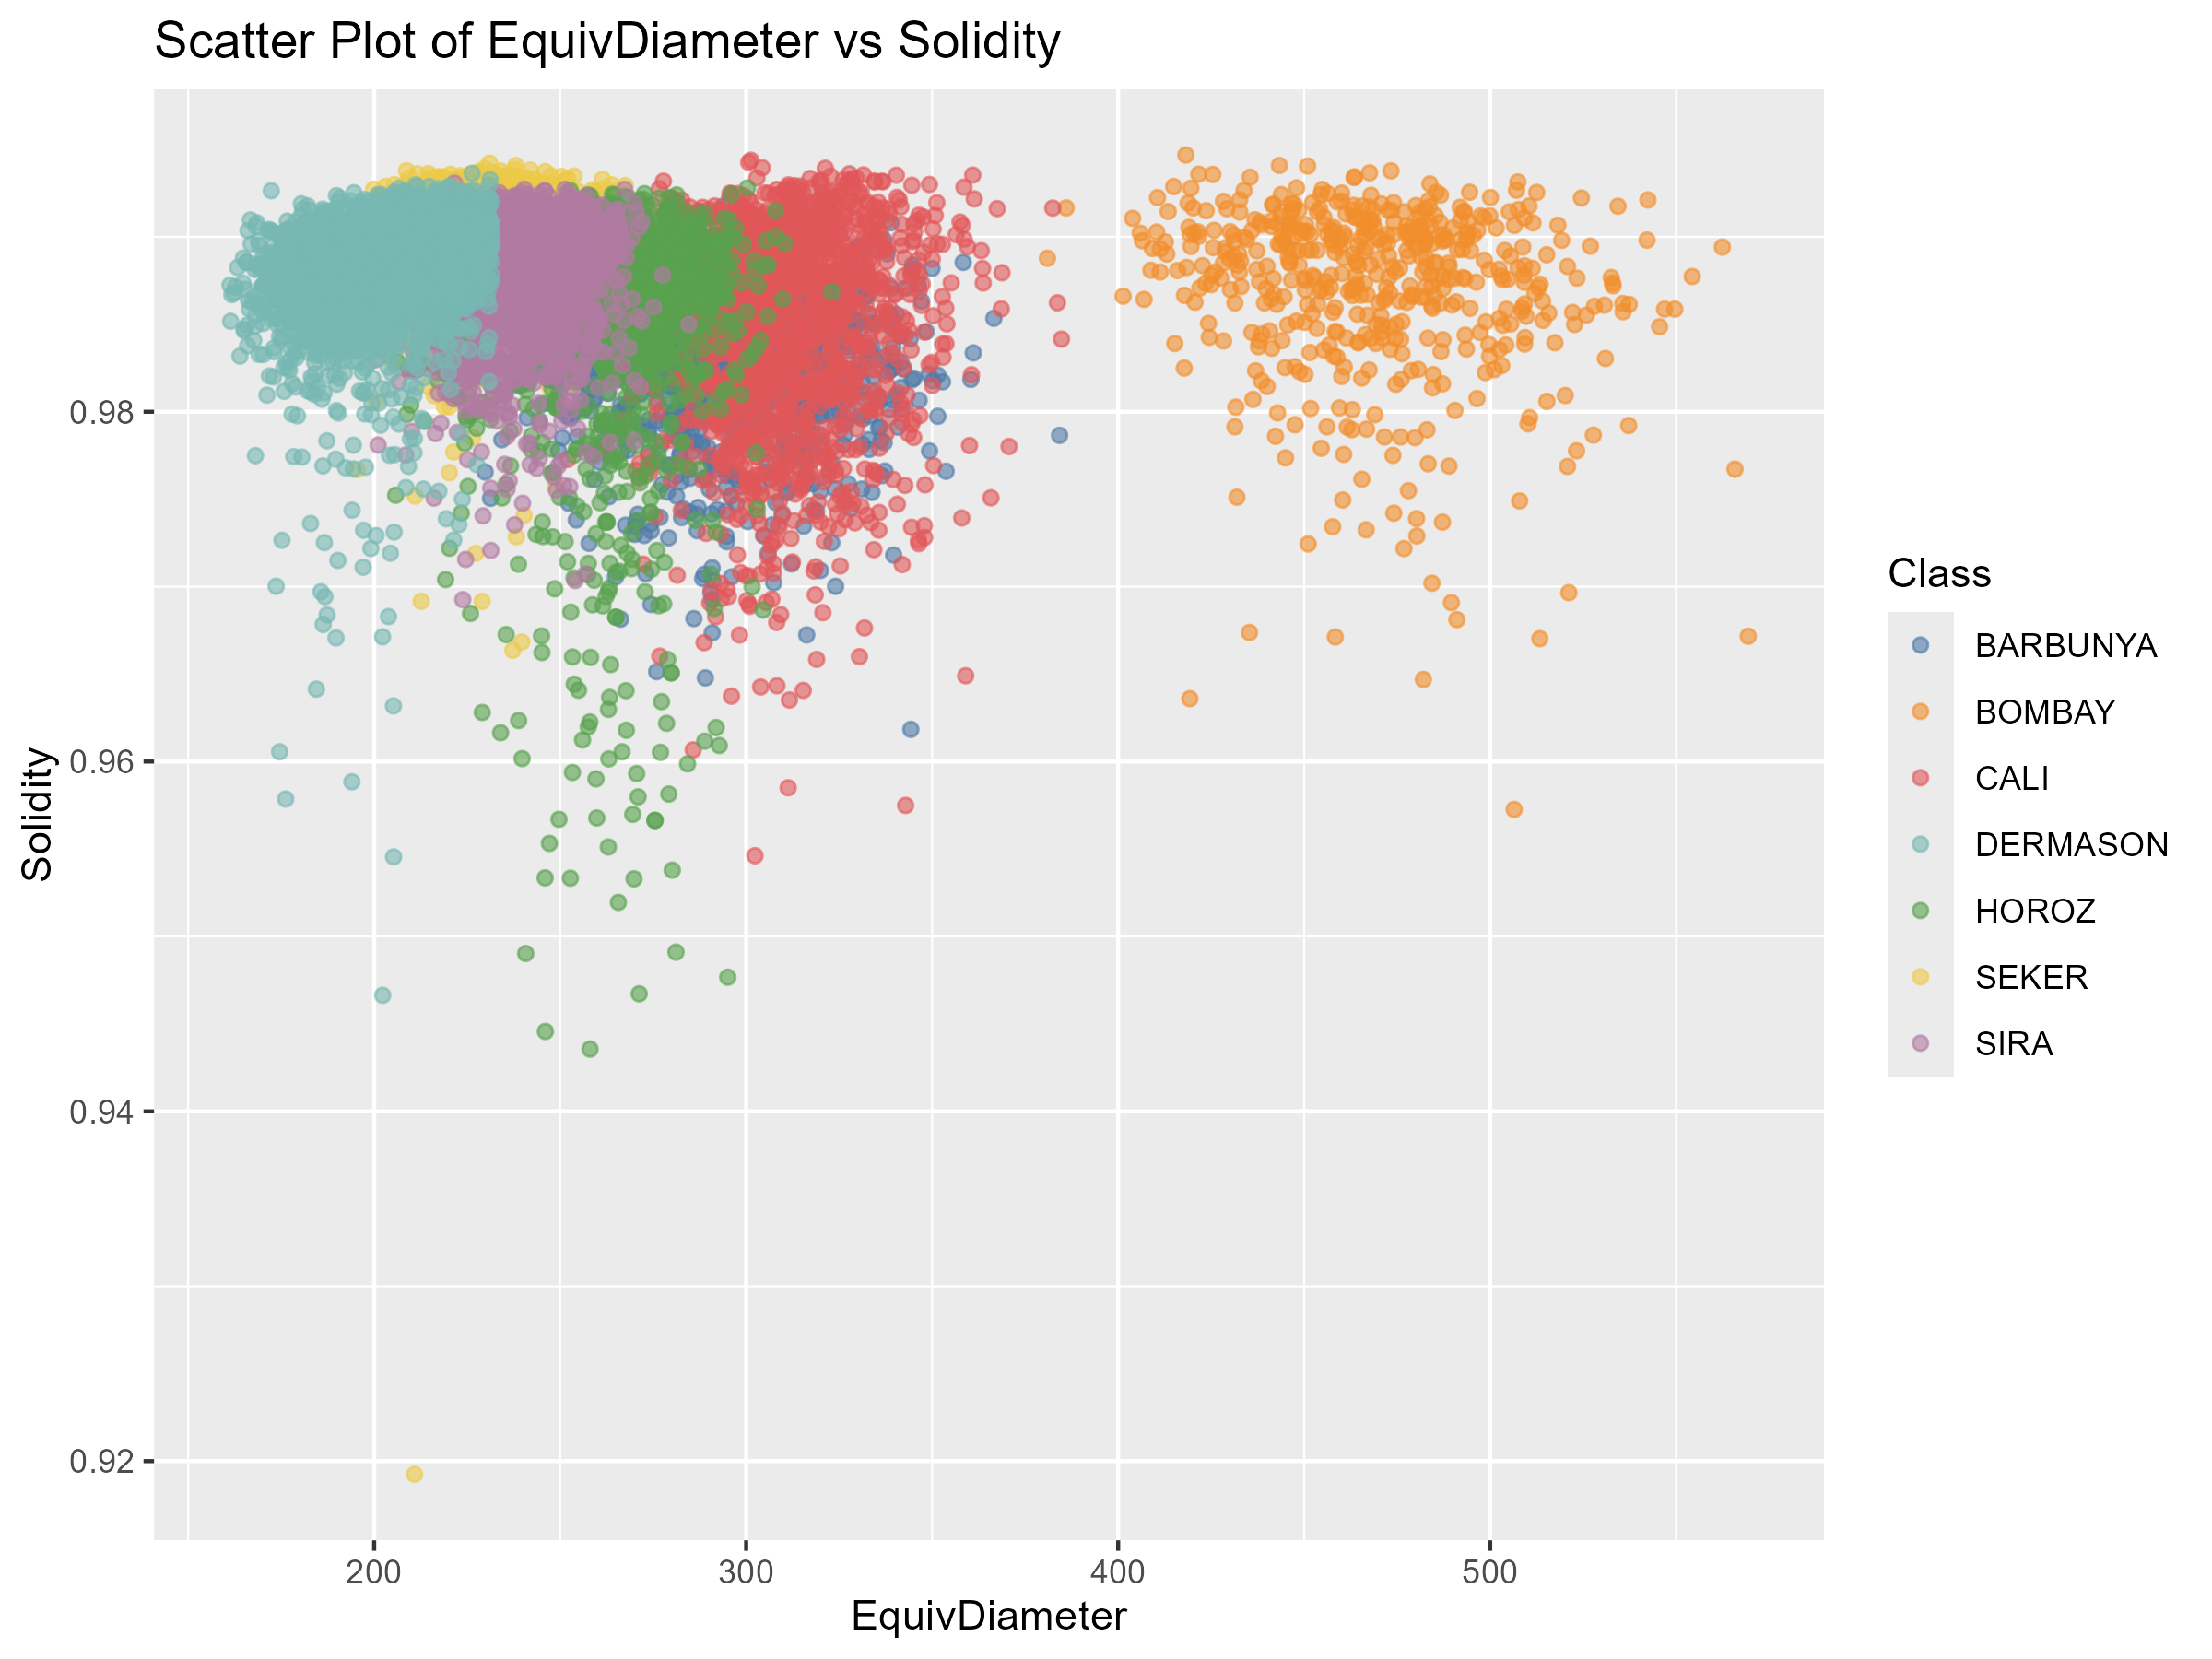
\includegraphics[width=0.8\textwidth]{graphs/scatter_equiv_solidity.png}
    \caption{Scatter Plot of EquivDiameter vs Solidity}
    \label{fig:scatter_equiv_solidity}
\end{figure}
This scatter plot shows the relationship between EquivDiameter and Solidity for different bean classes. The x-axis represents the equivalent diameter (EquivDiameter), while the y-axis shows the solidity values. Each point represents a bean instance, with colors differentiating the bean classes. Most points cluster in the range of EquivDiameter between 200 and 300, and Solidity values are generally high, ranging between 0.97 and 0.99. BOMBAY beans (orange) are spread farther along the EquivDiameter axis, having higher values compared to other classes. This plot highlights how solidity changes relative to the equivalent diameter across different bean types

\newpage

\subsection{Boxplot of Extent by Bean Class}
\noindent\textbf{Objective:} This boxplot compares the distribution of \textit{Extent} across different bean classes, answering: "How does the extent vary among the different bean types?"

\noindent\textbf{Explanation:} The plot shows the median, interquartile range, and outliers for the extent values of each bean class. Some classes exhibit higher median extent values, indicating a larger proportion of the convex hull occupied by the bean's area, while others show more variability or outliers, suggesting differences in shape compactness.

\begin{figure}[H]
    \centering
    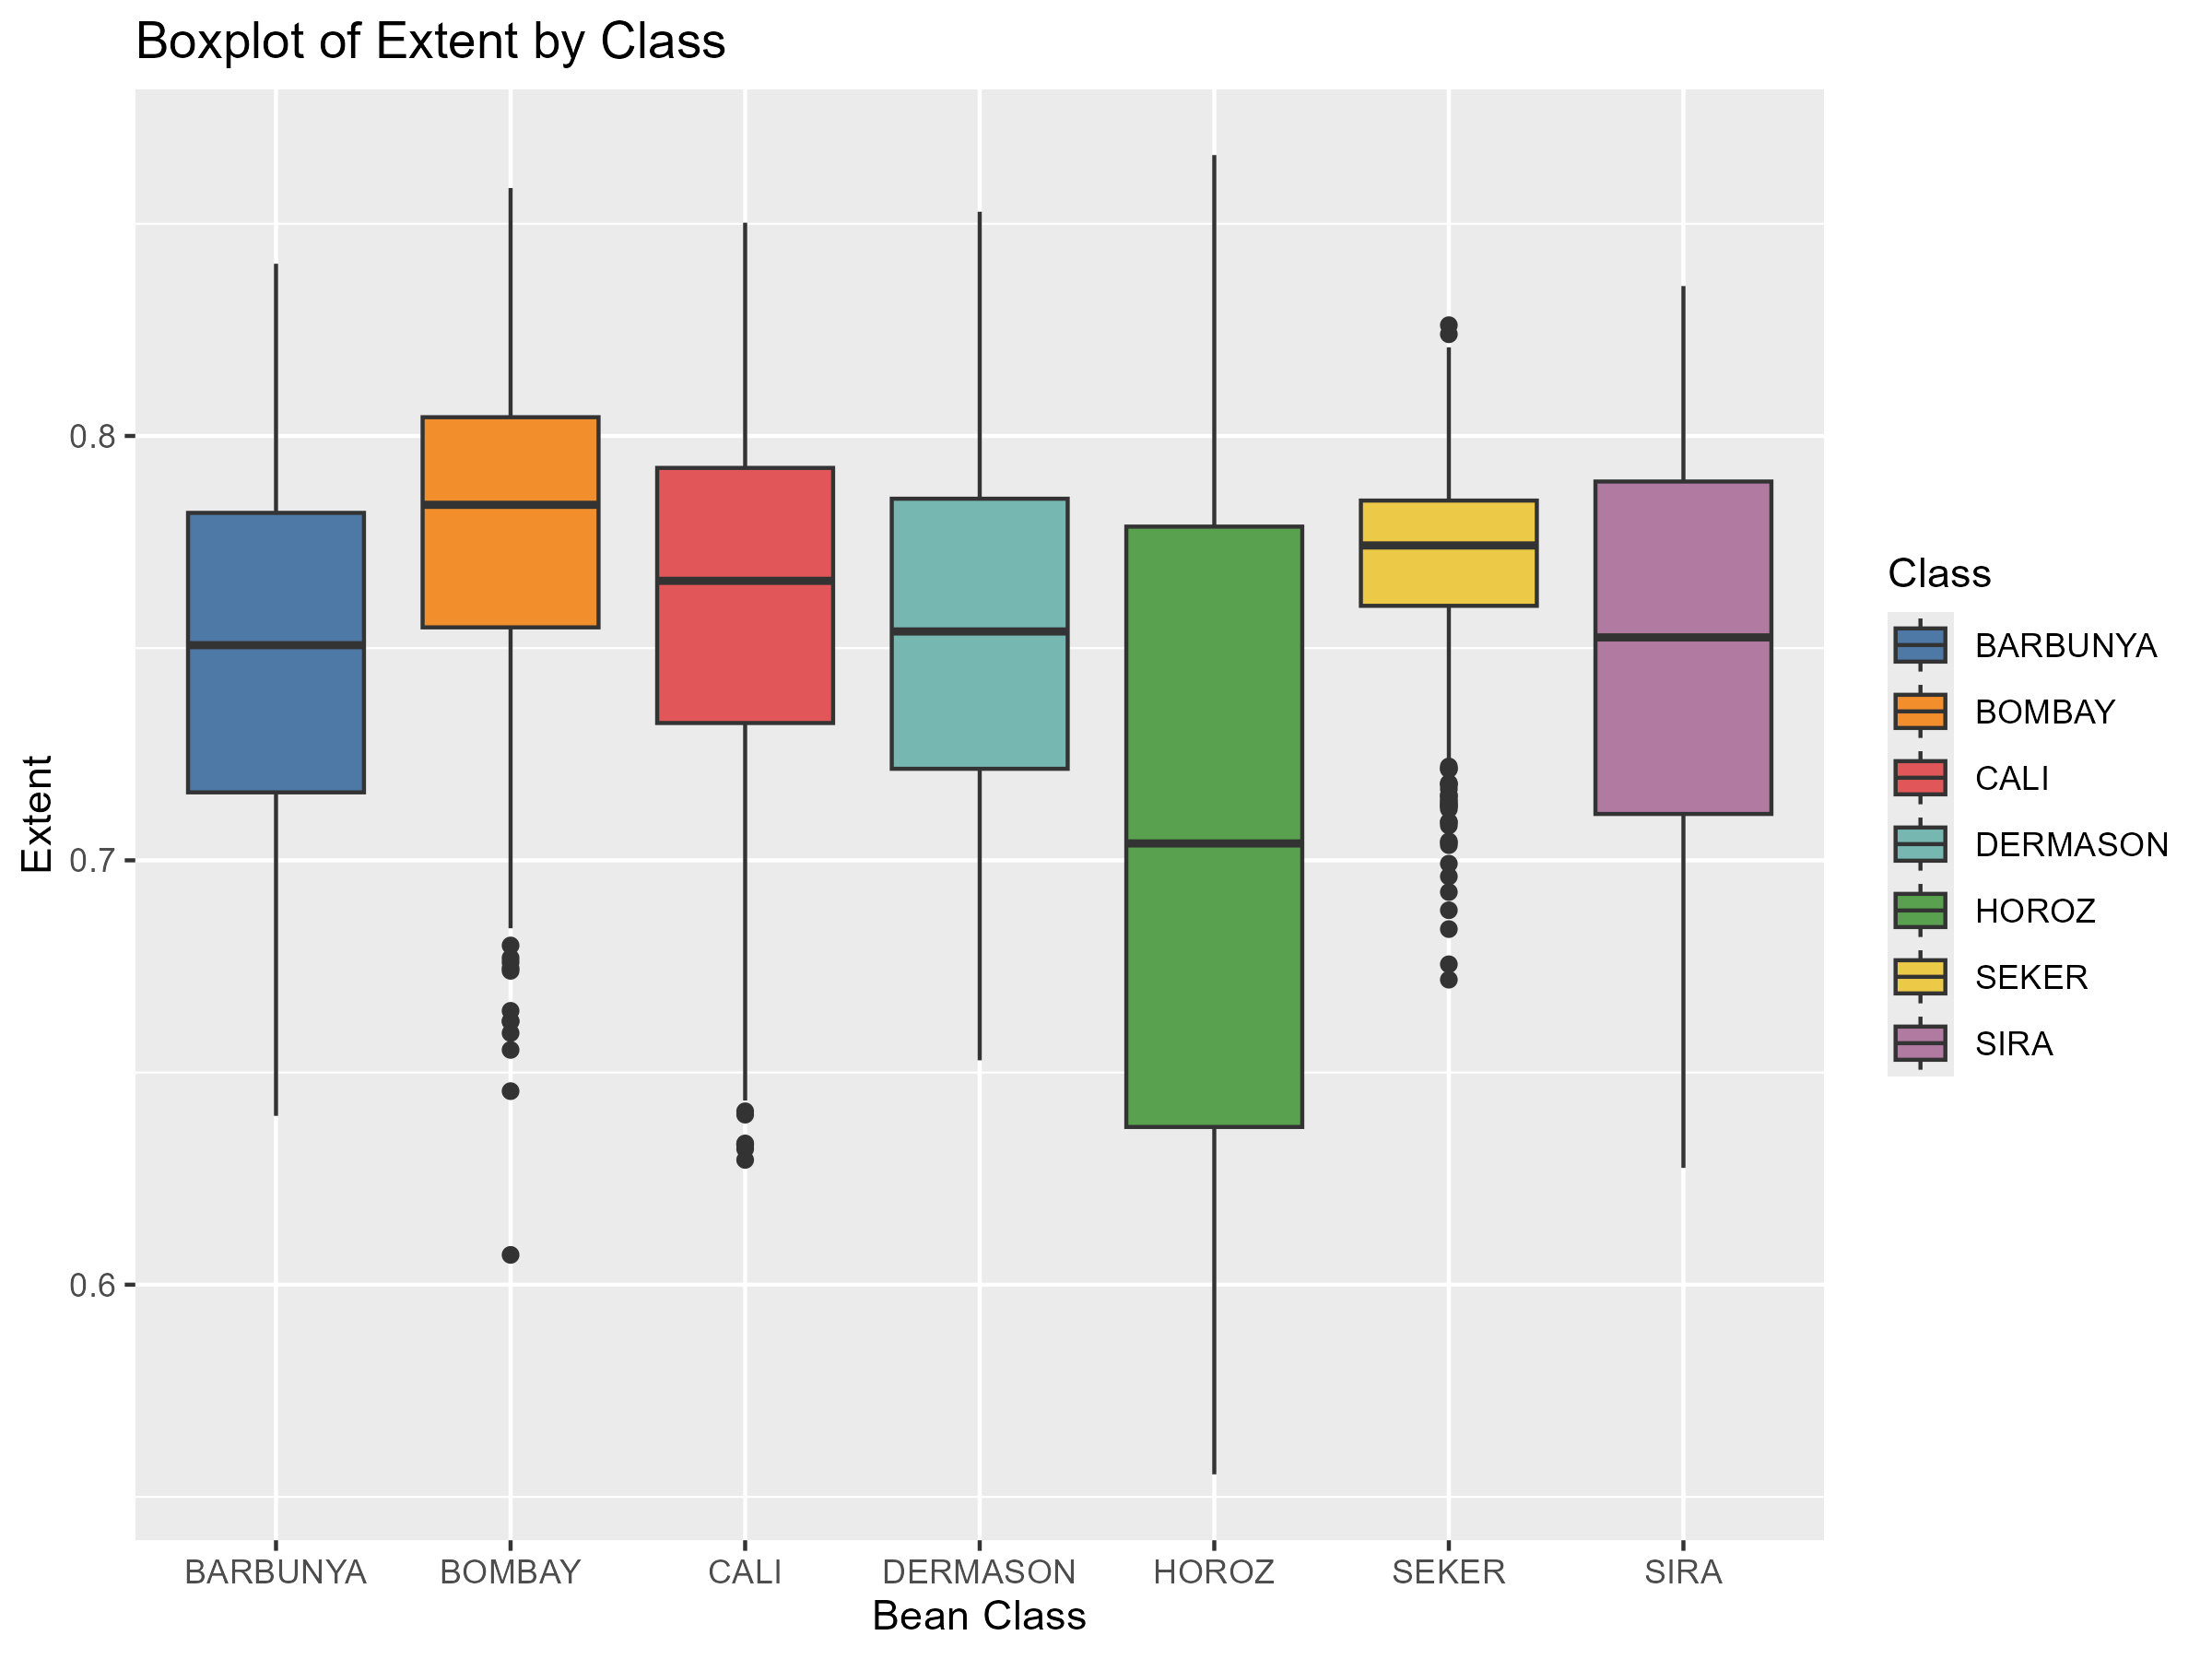
\includegraphics[width=0.8\textwidth]{graphs/boxplot_extent.png}
    \caption{Boxplot of Extent by Bean Class}
    \label{fig:boxplot_extent}
\end{figure}
This boxplot compares the distribution of Extent across different bean classes. The x-axis represents the bean classes, and the y-axis shows the extent values. The boxes indicate the interquartile range (IQR), with the middle line representing the median. HOROZ has the widest range of extent values, while other classes like BOMBAY and CALI have more compact distributions around higher values. SEKER has one outlier with a lower extent value.

\newpage

\subsection{Scatter Plot of Convex Area vs Area}
\noindent\textbf{Objective:} This scatter plot examines the relationship between \textit{Convex Area} and \textit{Area} across different bean classes, answering: "Is there a strong correlation between convex area and area?"

\noindent\textbf{Explanation:} The plot shows a positive correlation between \textit{Convex Area} and \textit{Area}, indicating that as one increases, the other tends to increase as well.

\begin{figure}[H]
    \centering
    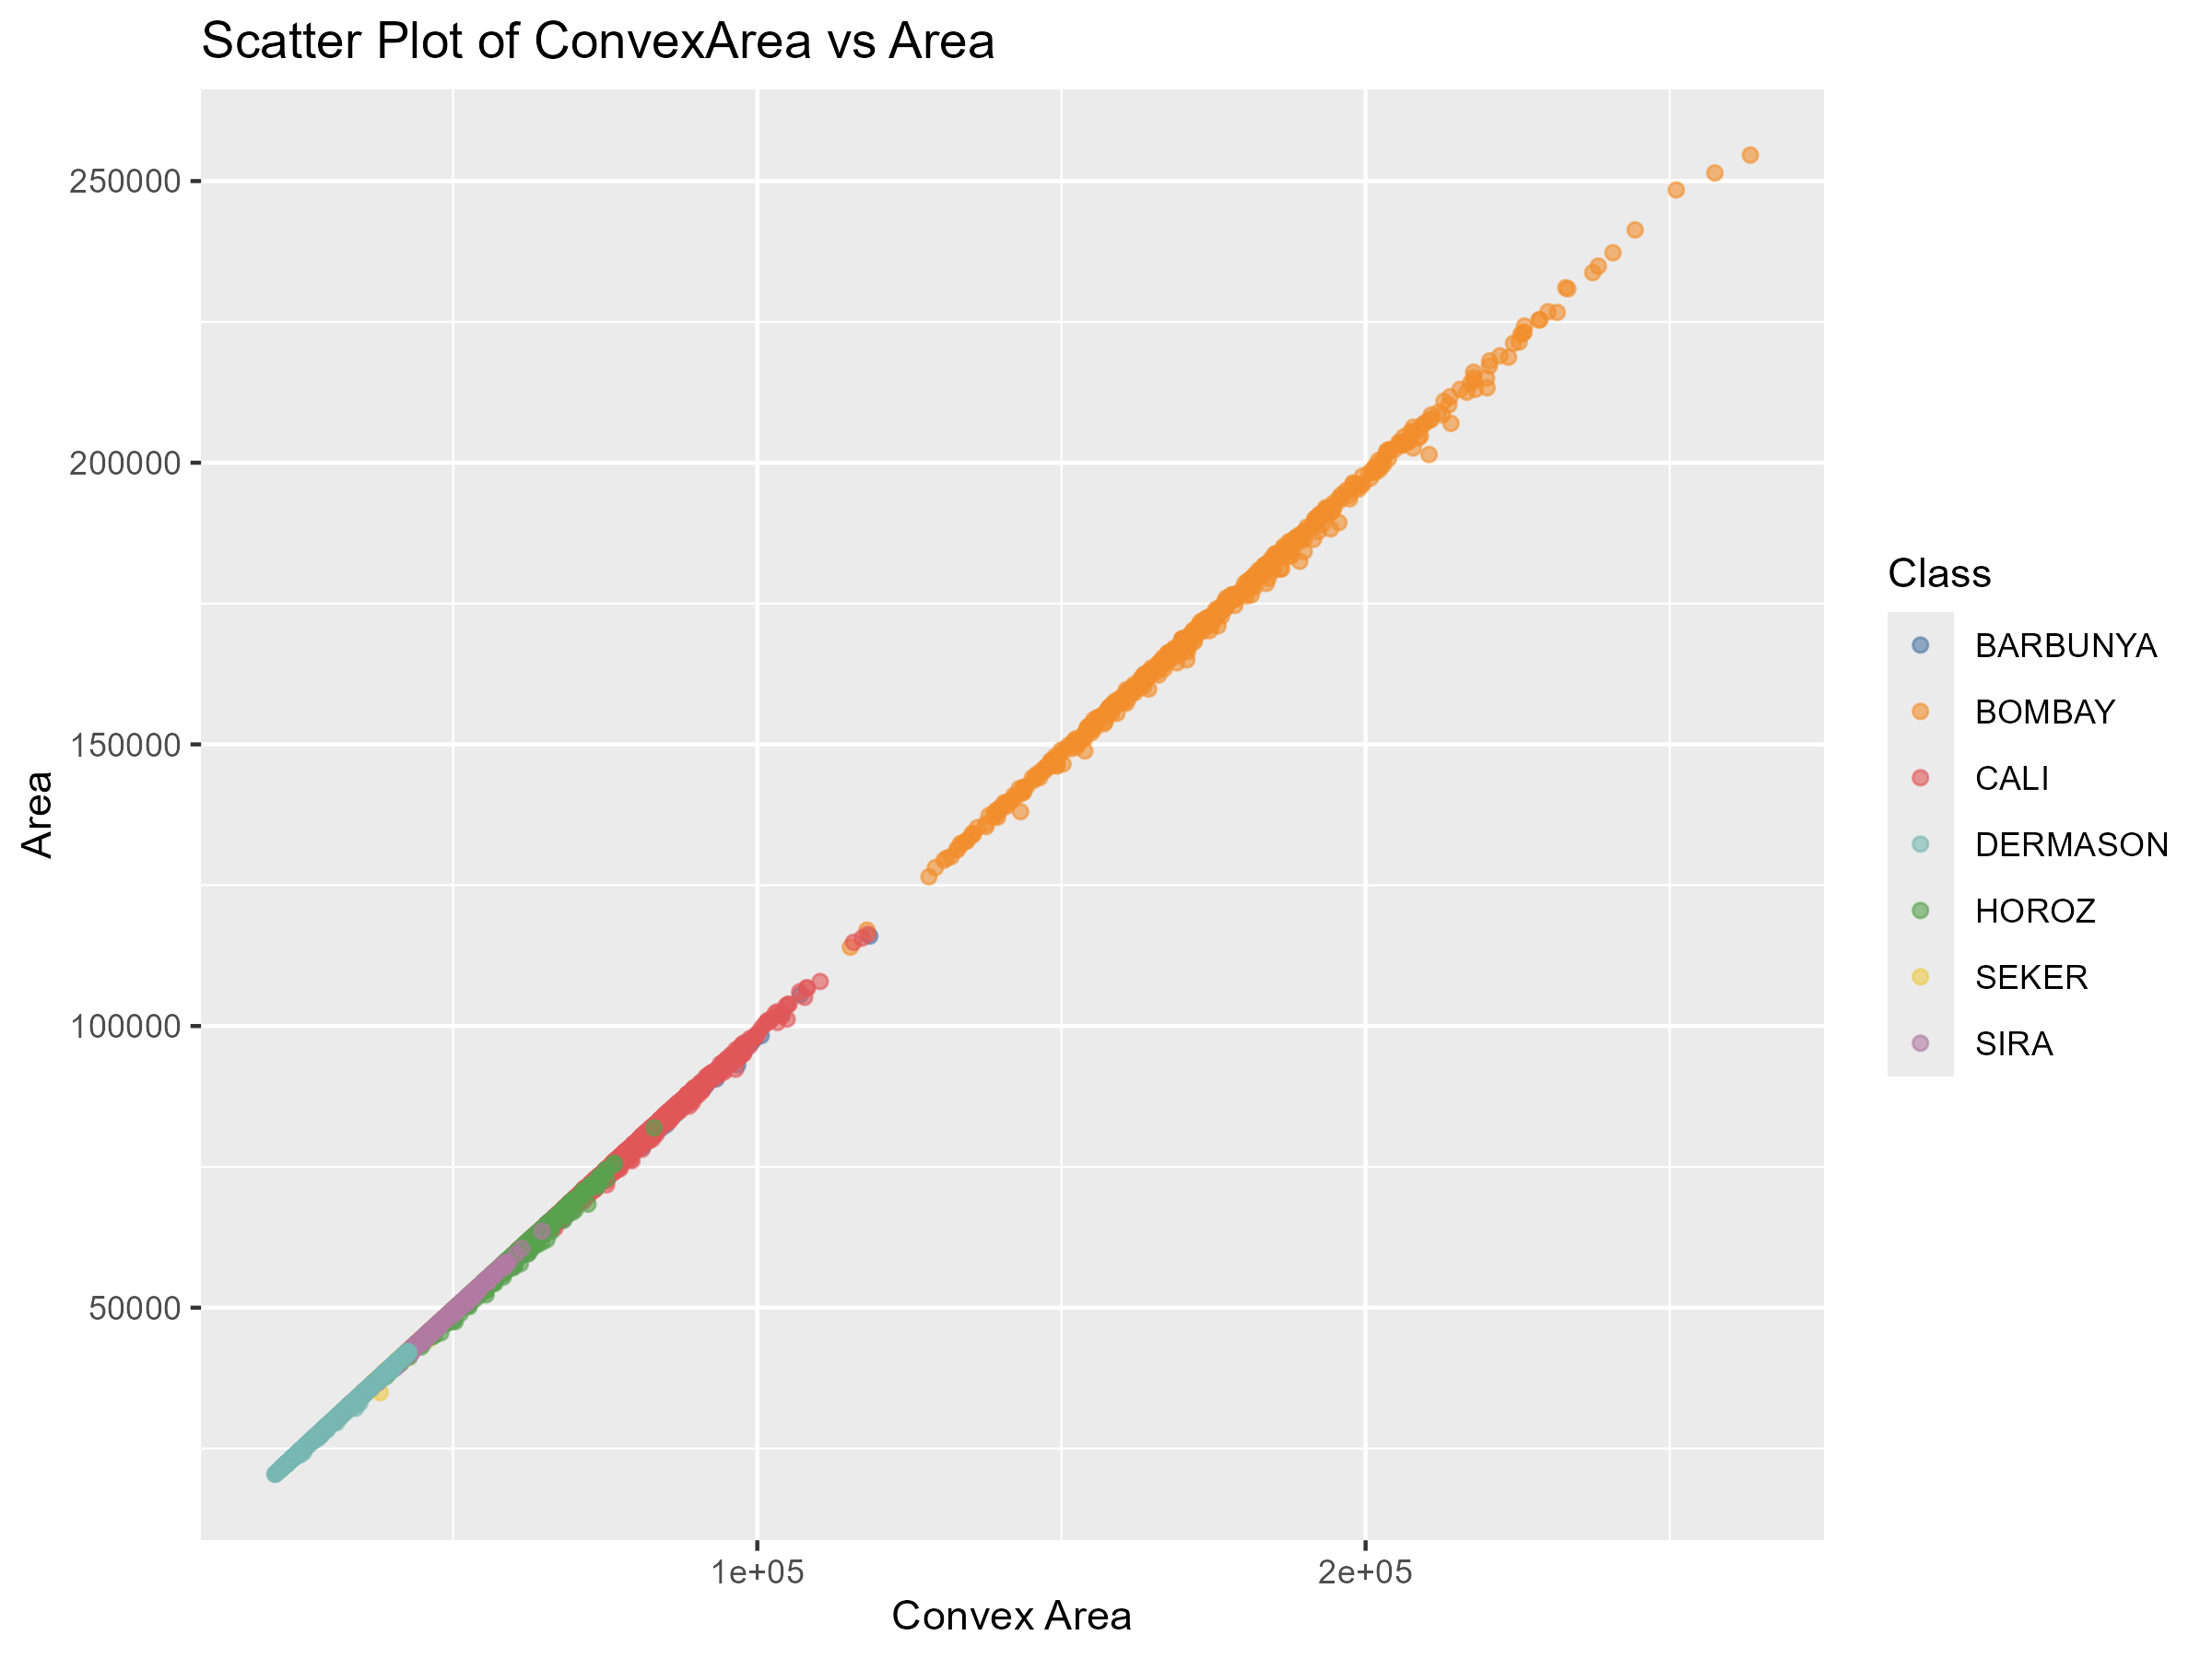
\includegraphics[width=0.8\textwidth]{graphs/scatter_convexarea_area.png}
    \caption{Scatter Plot of Convex Area vs Area}
    \label{fig:scatter_convex_area}
\end{figure}
This scatter plot shows the relationship between ConvexArea and Area for different bean classes. The x-axis represents ConvexArea, while the y-axis shows Area. Each point represents a bean instance, with colors indicating the bean class. There is a strong positive linear correlation between the two variables, meaning as the convex area increases, the regular area also increases proportionally. BOMBAY beans (orange) have higher values for both ConvexArea and Area compared to other classes, while the rest of the classes cluster together in the lower range.

\newpage

\subsection{Histogram of Eccentricity}
\noindent\textbf{Objective:} This histogram displays the distribution of \textit{Eccentricity} values in the dataset, answering: "What are the common eccentricity ranges for the beans?"

\noindent\textbf{Explanation:} The histogram shows that most beans have eccentricity values concentrated between 0.6 and 0.8, suggesting moderate elongation.

\begin{figure}[H]
    \centering
    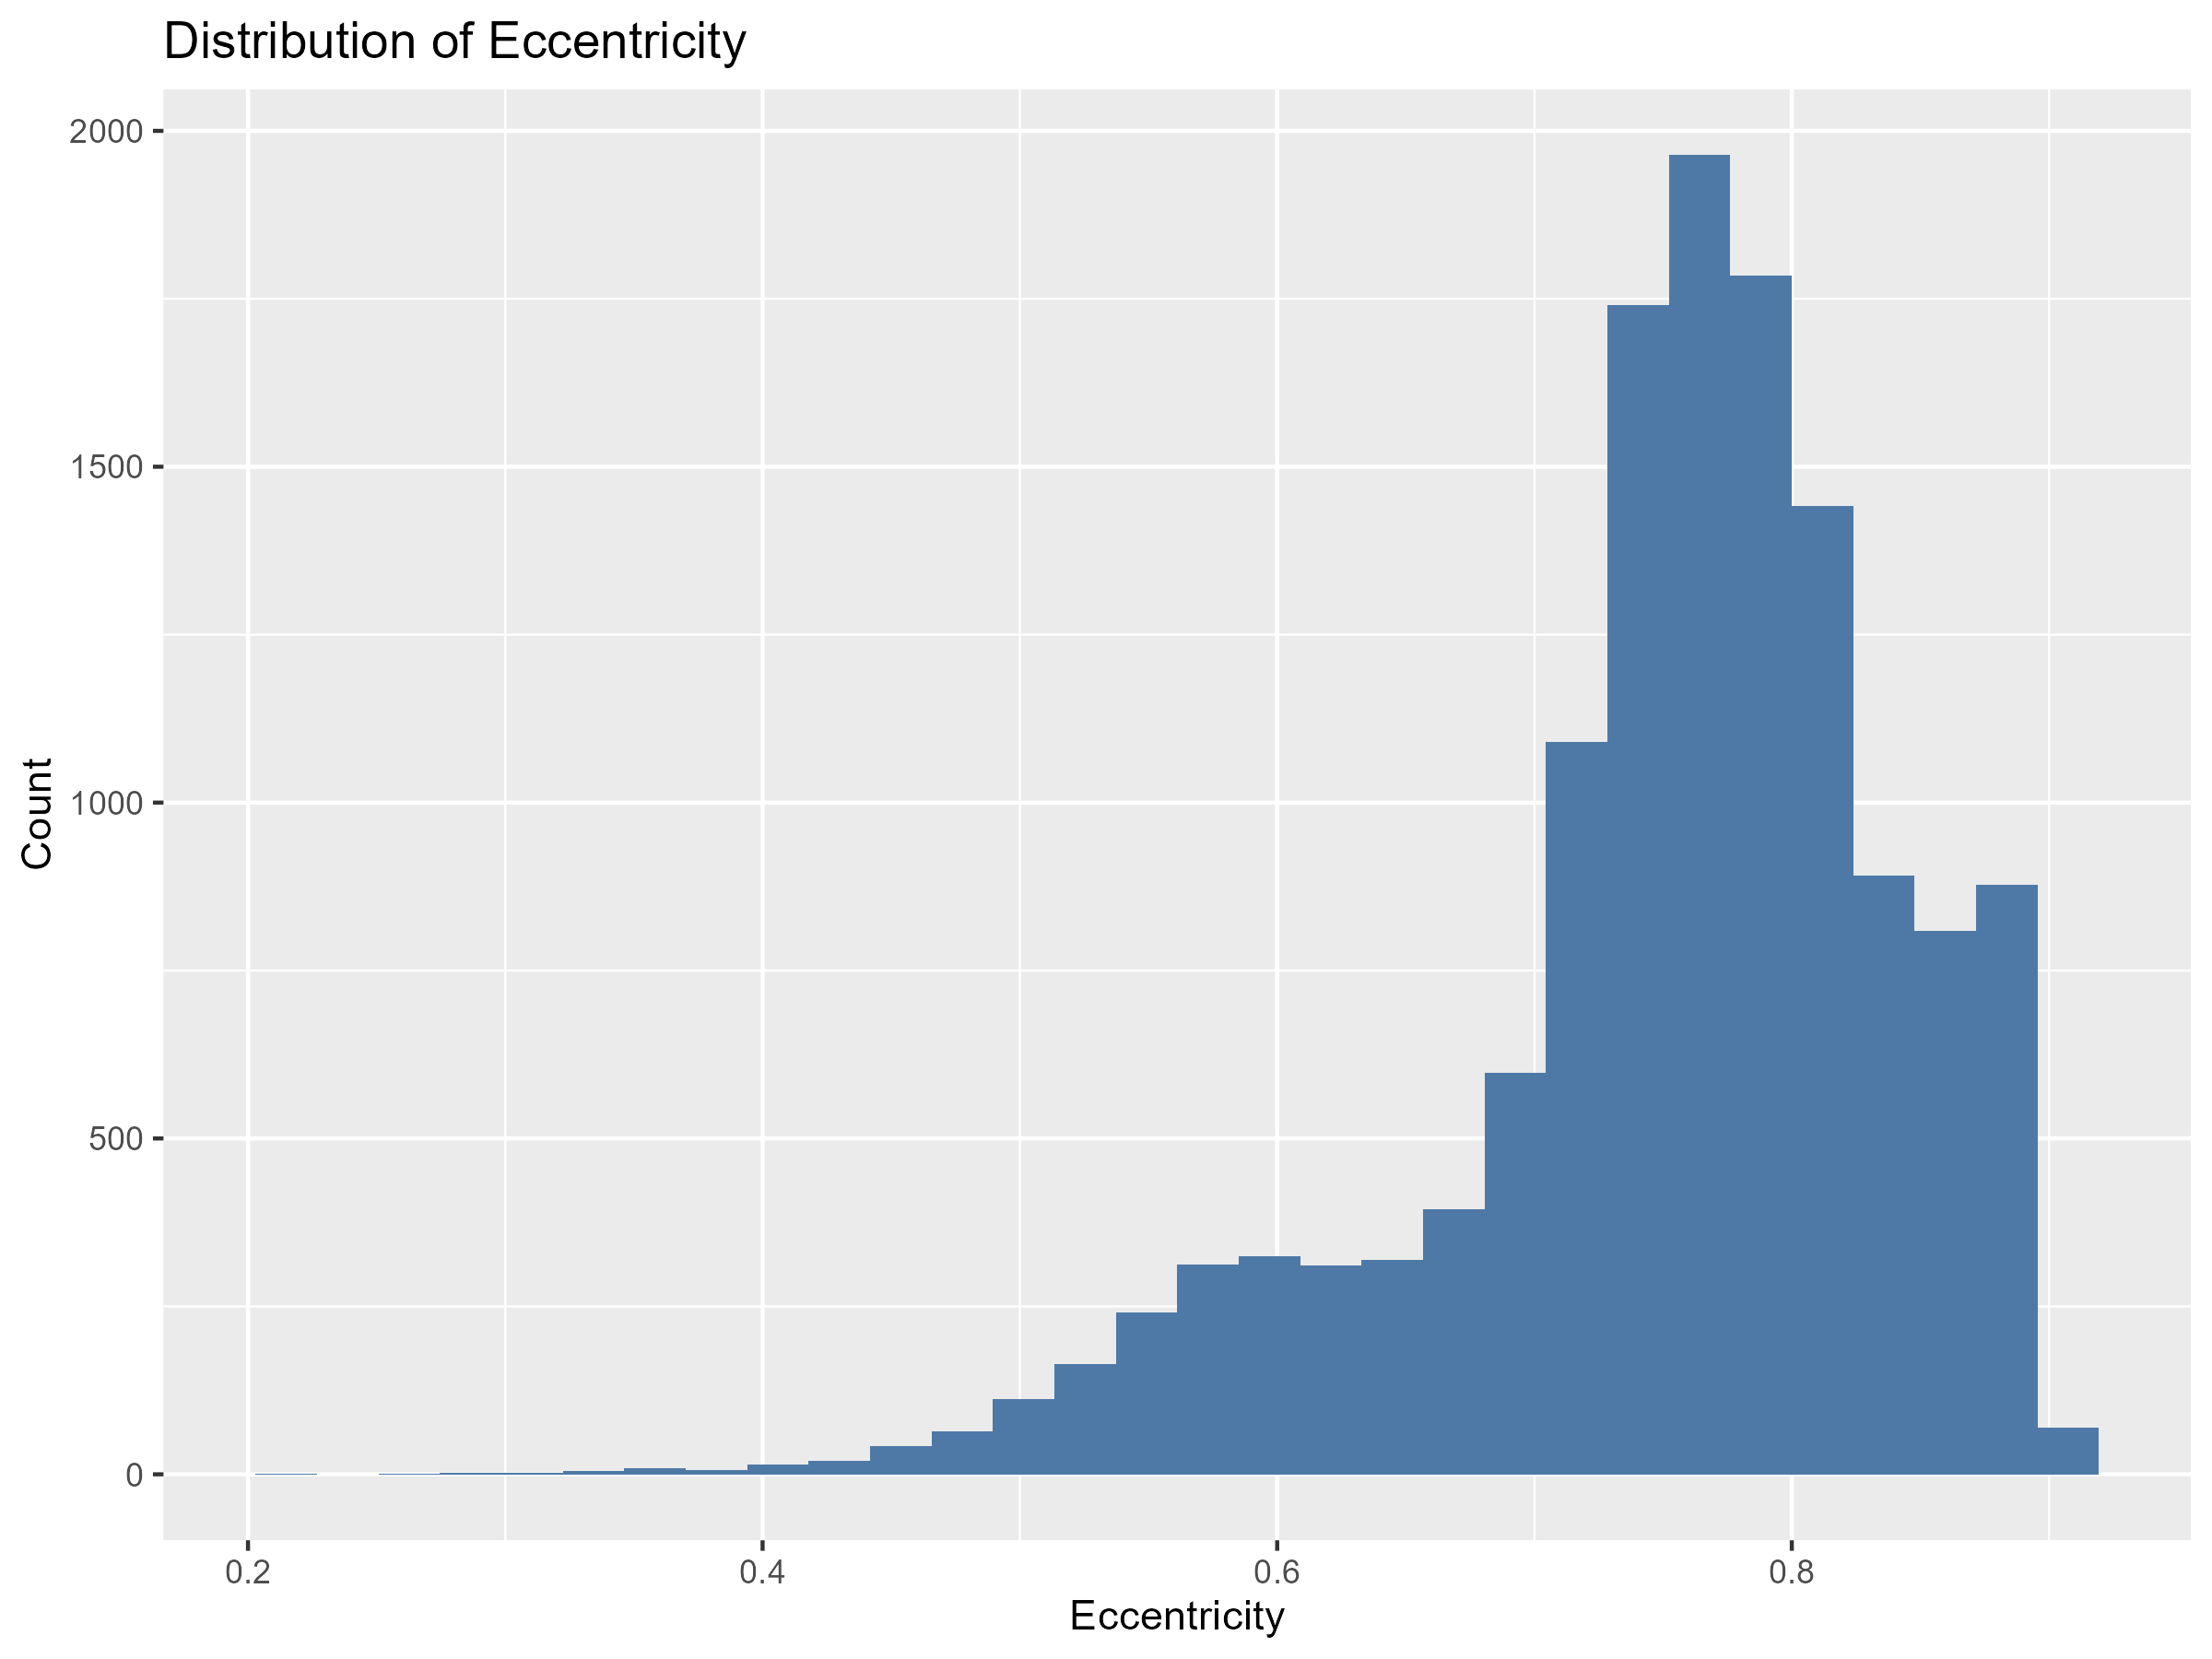
\includegraphics[width=0.8\textwidth]{graphs/histogram_eccentricity.png}
    \caption{Histogram of Eccentricity}
    \label{fig:histogram_eccentricity}
\end{figure}
This histogram displays the distribution of Eccentricity values in the dataset. The x-axis represents eccentricity values, while the y-axis shows the count of instances for each value range. Most of the data points are concentrated between 0.6 and 0.8, with the highest count occurring around 0.7. There are fewer instances at lower eccentricity values (below 0.5) and higher values (above 0.9). This plot highlights that most bean instances have moderately high eccentricity, indicating their deviation from being perfectly circular.

\newpage

\subsection{Scatter Plot of Perimeter vs Aspect Ratio}
\noindent\textbf{Objective:} This scatter plot shows the relationship between \textit{Perimeter} and \textit{Aspect Ratio}, answering: "Is there a relationship between a bean's perimeter and its aspect ratio?"

\noindent\textbf{Explanation:} The scatter plot reveals that beans with larger perimeters tend to have higher aspect ratios, indicating a possible relationship between these two features.

\begin{figure}[H]
    \centering
    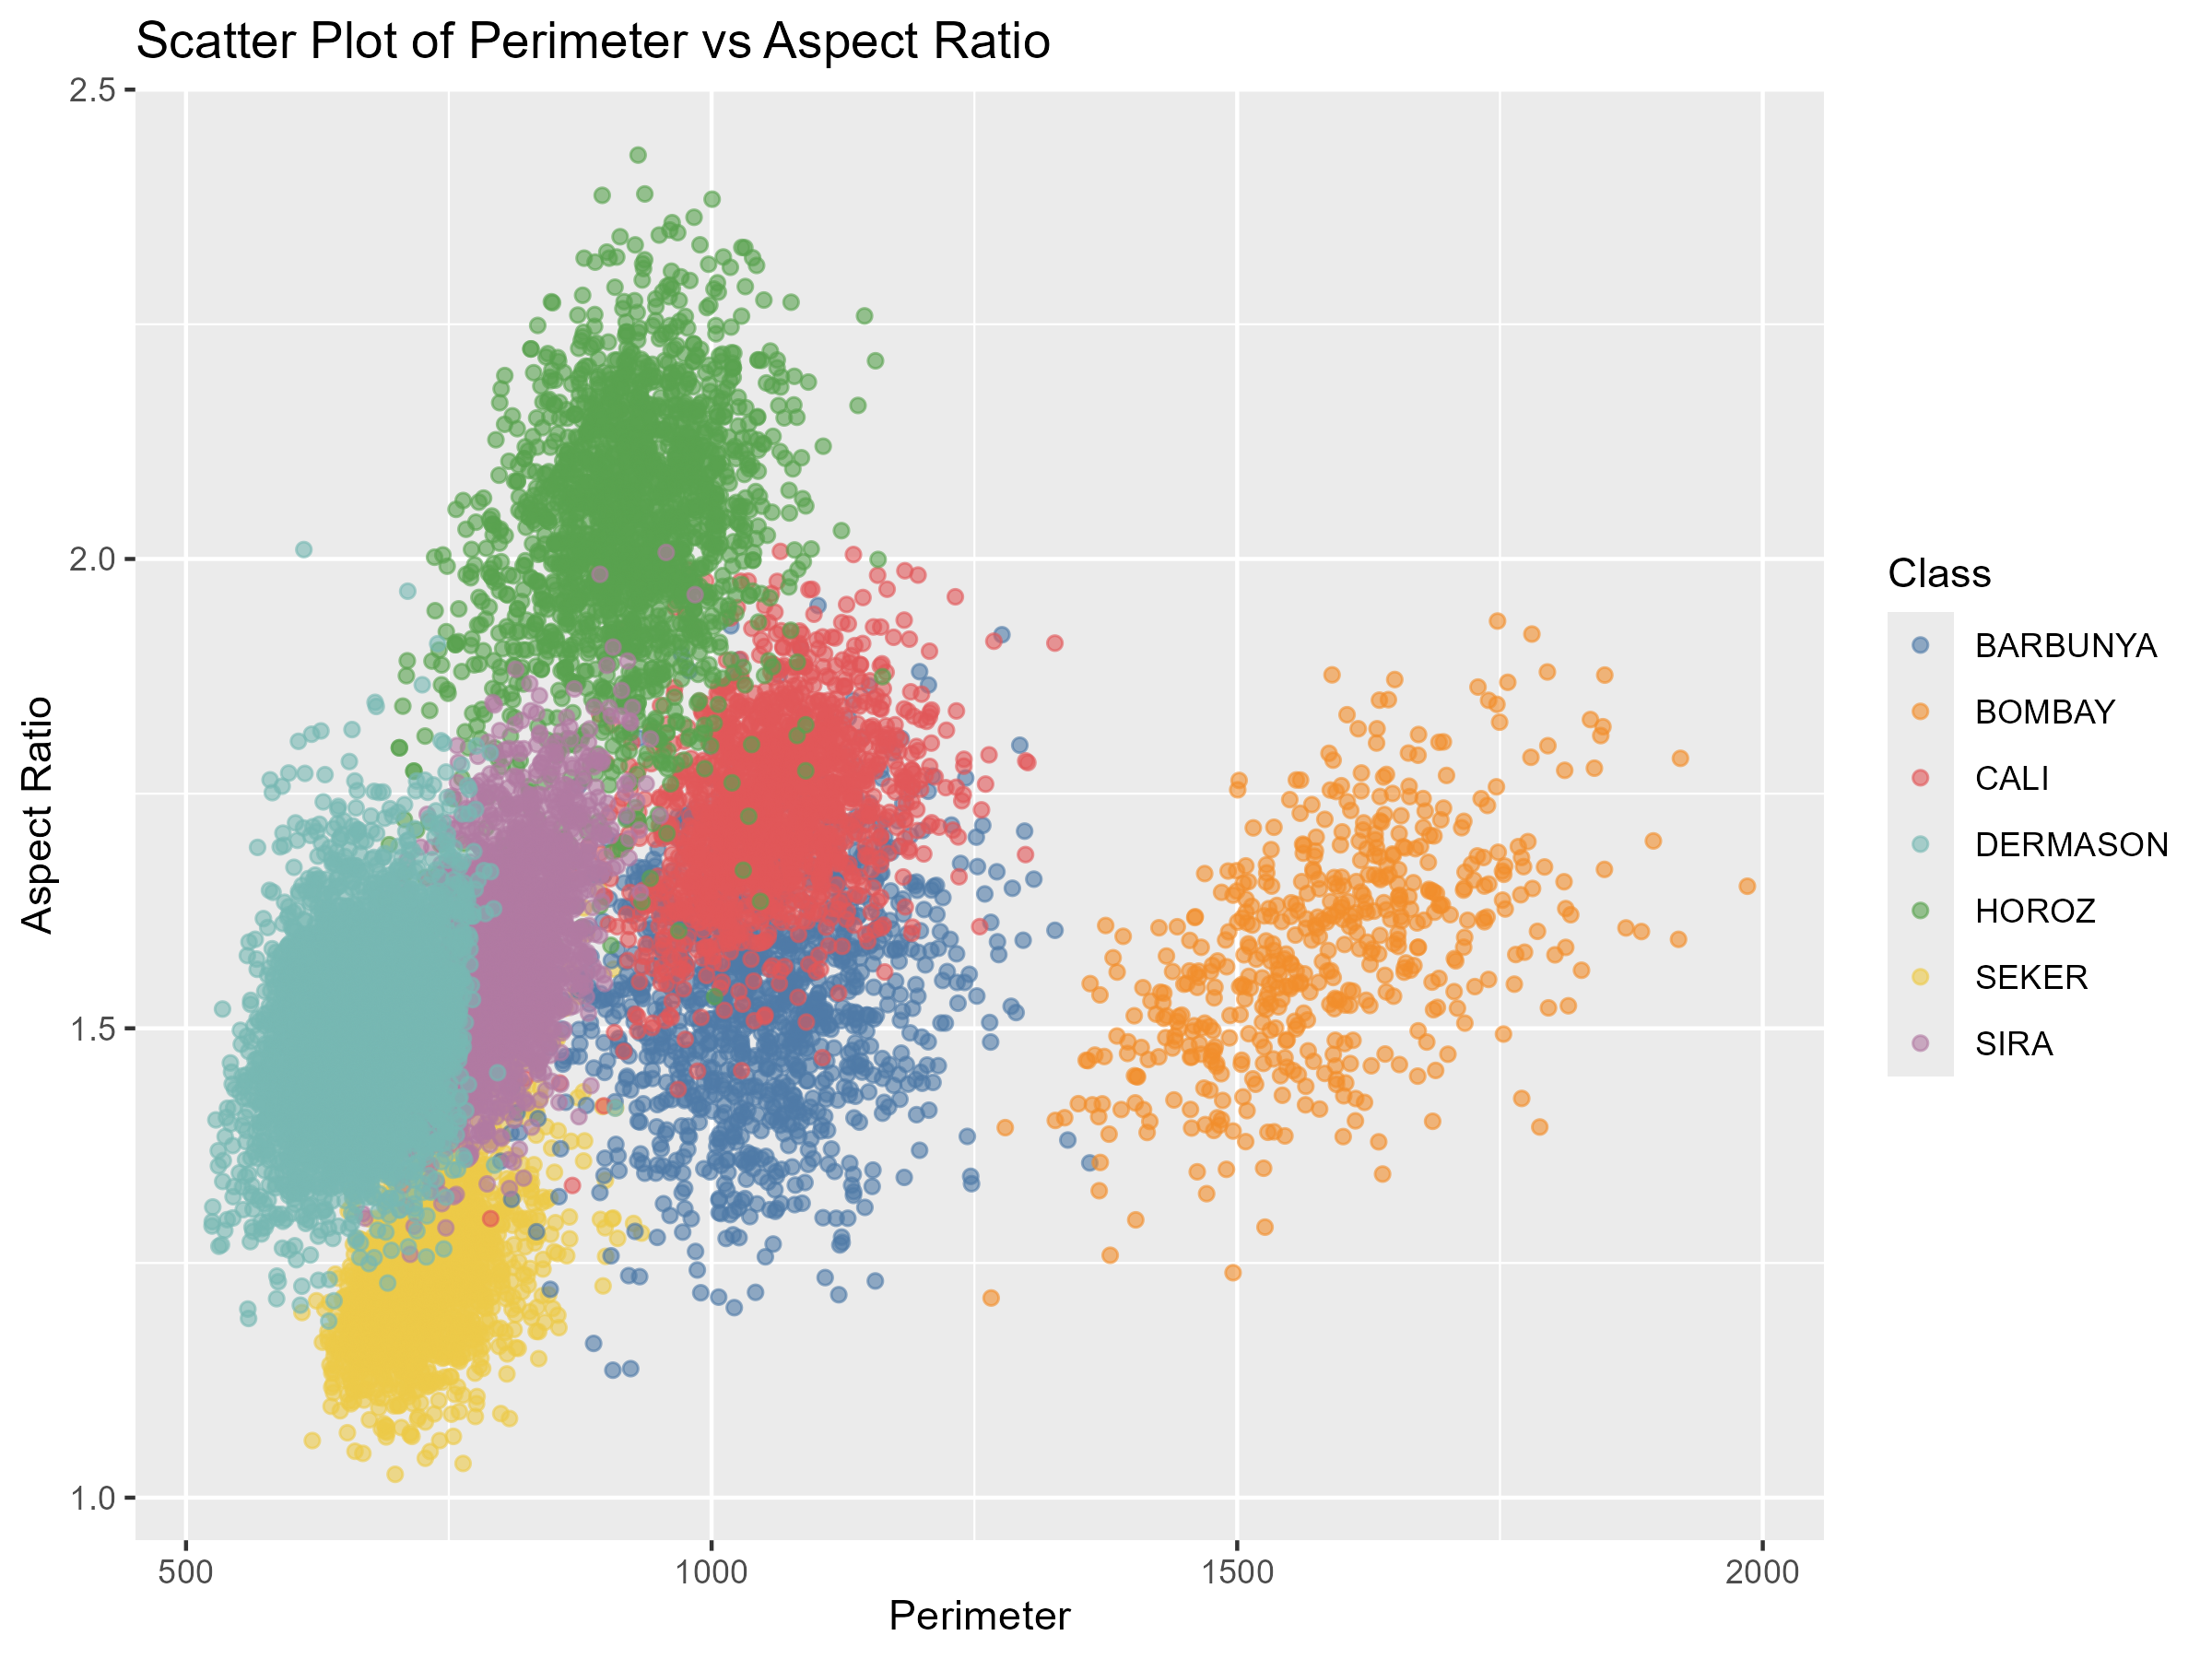
\includegraphics[width=0.8\textwidth]{graphs/scatter_perimeter_aspectratio.png}
    \caption{Scatter Plot of Perimeter vs Aspect Ratio}
    \label{fig:scatter_perimeter_aspect}
\end{figure}
This scatter plot shows the relationship between Perimeter and Aspect Ratio for different bean classes. The x-axis represents Perimeter, while the y-axis represents Aspect Ratio. The plot helps in understanding how the Perimeter of beans is related to their Aspect Ratio.

\newpage

\subsection{Boxplot of EquivDiameter by Bean Class}
\noindent\textbf{Objective:} This boxplot visualizes the distribution of \textit{EquivDiameter} across different bean classes, answering: "How does the equivalent diameter differ among bean types?"

\noindent\textbf{Explanation:} The plot shows that BOMBAY beans have a higher median equivalent diameter compared to other classes, indicating larger overall sizes.

\begin{figure}[H]
    \centering
    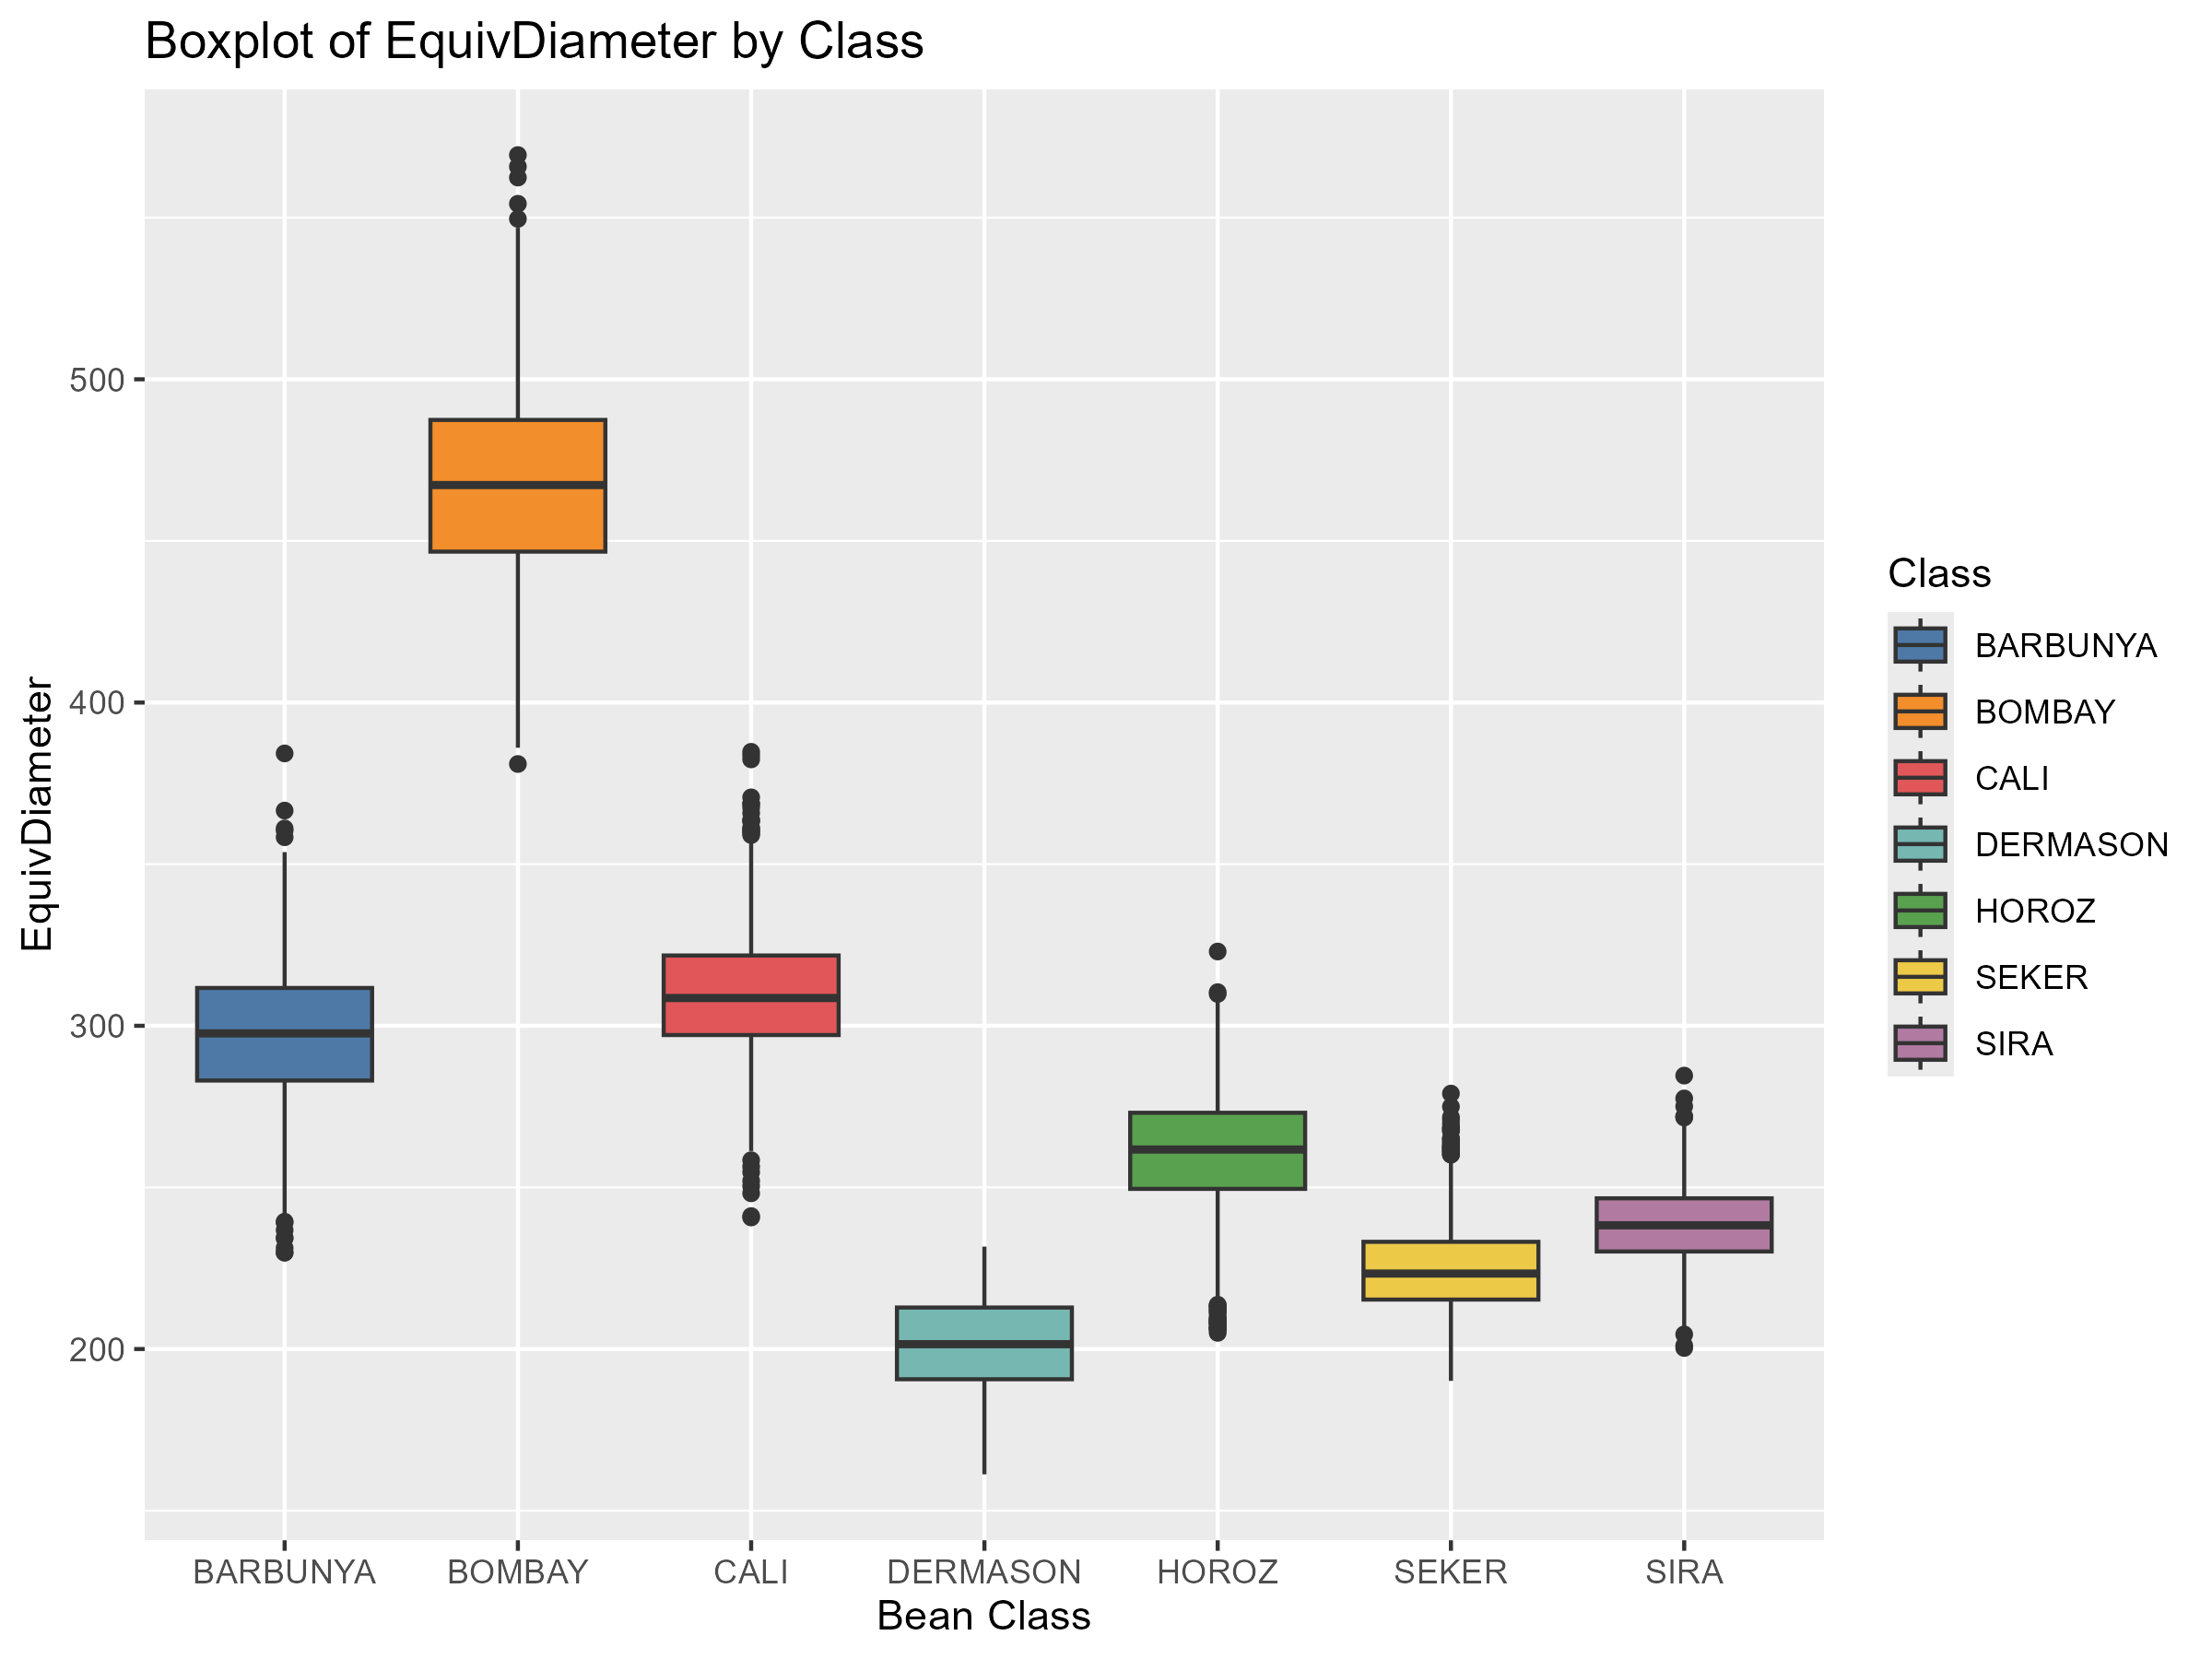
\includegraphics[width=0.8\textwidth]{graphs/boxplot_equivdiameter.png}
    \caption{Boxplot of EquivDiameter by Bean Class}
    \label{fig:boxplot_equivdiameter}
\end{figure}
This boxplot illustrates the distribution of EquivDiameter across different bean classes. The x-axis represents the bean classes, and the y-axis shows the equivalent diameter values. BOMBAY beans have the largest median EquivDiameter with a wider range, while SEKER and SIRA beans have smaller median values and tighter distributions. BARBUNYA has a few outliers on the lower end, and CALI shows more variability compared to other classes.

\newpage

\subsection{Density Plot of ShapeFactor1 by Bean Class}
\noindent\textbf{Objective:} This density plot illustrates the distribution of \textit{ShapeFactor1} across different bean classes, answering: "How does ShapeFactor1 vary among the different bean types?"

\noindent\textbf{Explanation:} The density plot shows that some bean classes have distinct peaks at certain ShapeFactor1 values, while others exhibit broader distributions. These variations can help in distinguishing the shape characteristics that are unique to different bean classes.

\begin{figure}[H]
    \centering
    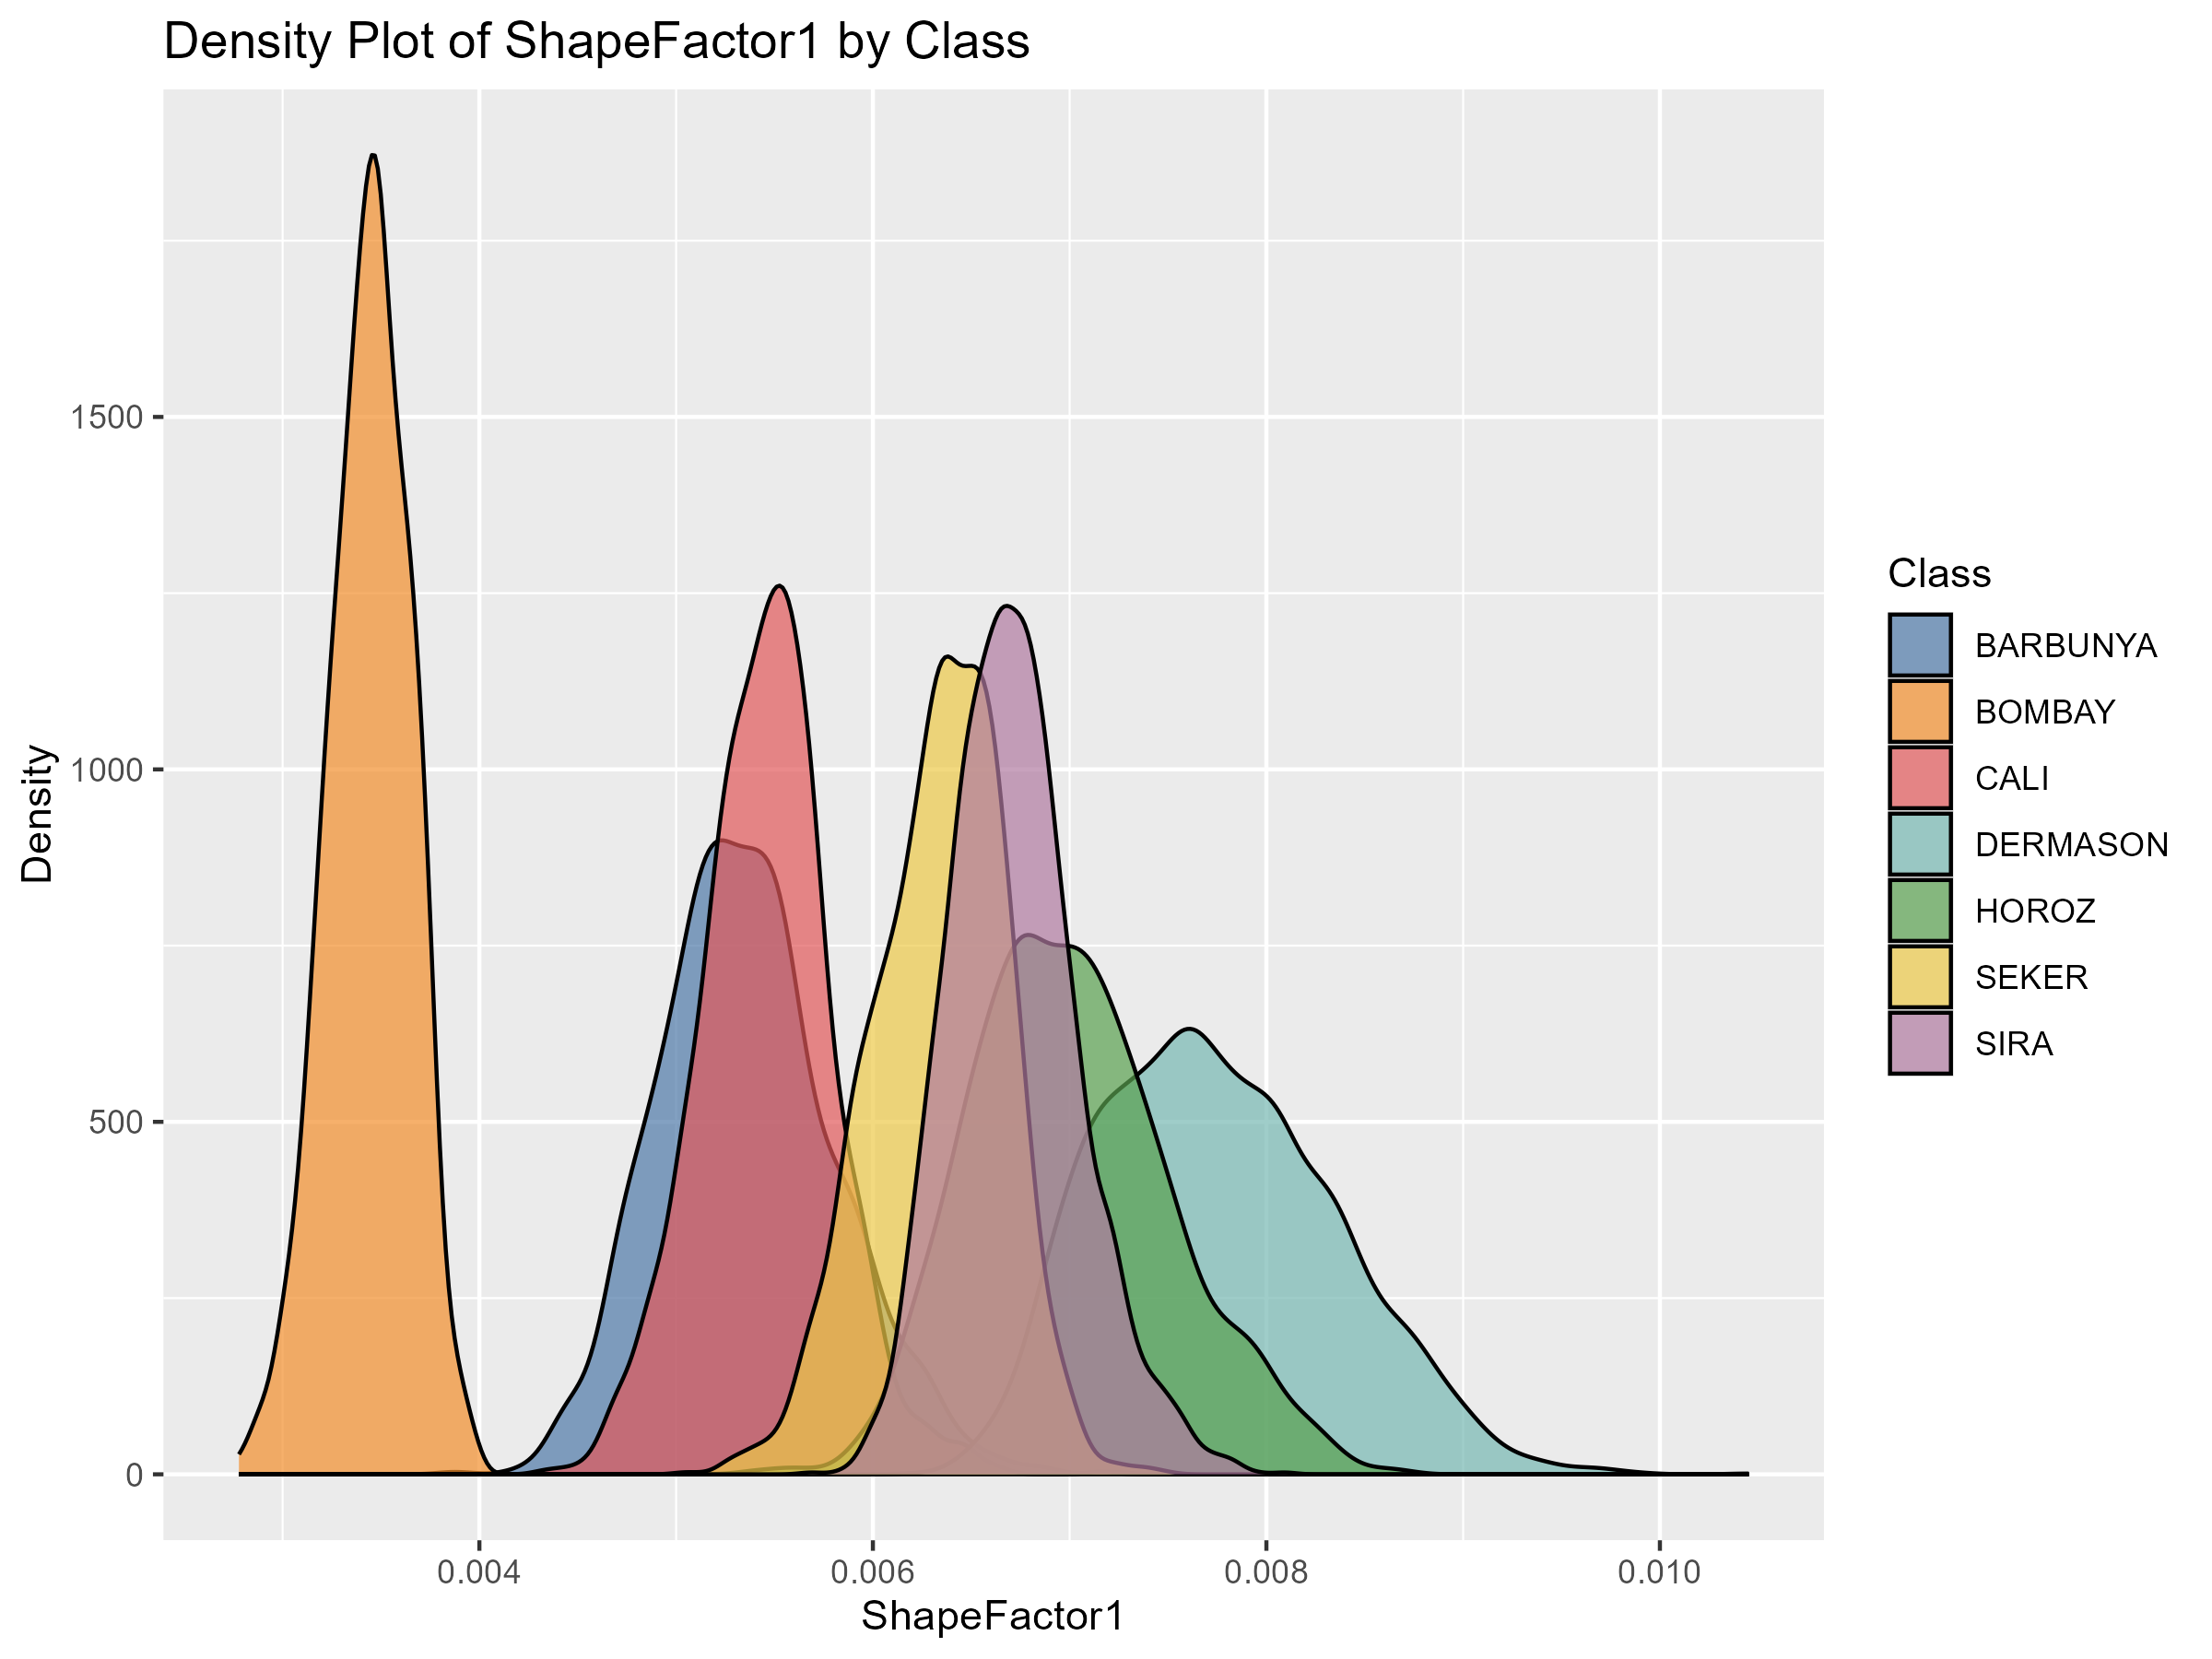
\includegraphics[width=0.8\textwidth]{graphs/density_shapefactor1.png}
    \caption{Density Plot of ShapeFactor1 by Bean Class}
    \label{fig:density_shapefactor1}
\end{figure}
This density plot shows the distribution of ShapeFactor1 for different bean classes. The x-axis represents the ShapeFactor1 values, and the y-axis indicates the density of instances for each class. BOMBAY beans (orange) have a distinct peak around 0.004, indicating most of their ShapeFactor1 values are clustered in this range. Other classes, such as CALI and SIRA, overlap around 0.005, while DERMASON and HOROZ have higher ShapeFactor1 values, peaking closer to 0.008.

\newpage

\subsection{Histogram of ShapeFactor4}
\noindent\textbf{Objective:} This histogram illustrates the distribution of \textit{ShapeFactor4} values across the dataset, answering: "What are the common ranges for ShapeFactor4 among the bean types?"

\noindent\textbf{Explanation:} The histogram shows the frequency of ShapeFactor4 values for all bean classes. The distribution reveals whether most beans fall within a narrow range or if there is significant variability, indicating differences in the geometric properties associated with ShapeFactor4 across the dataset.

\begin{figure}[H]
    \centering
    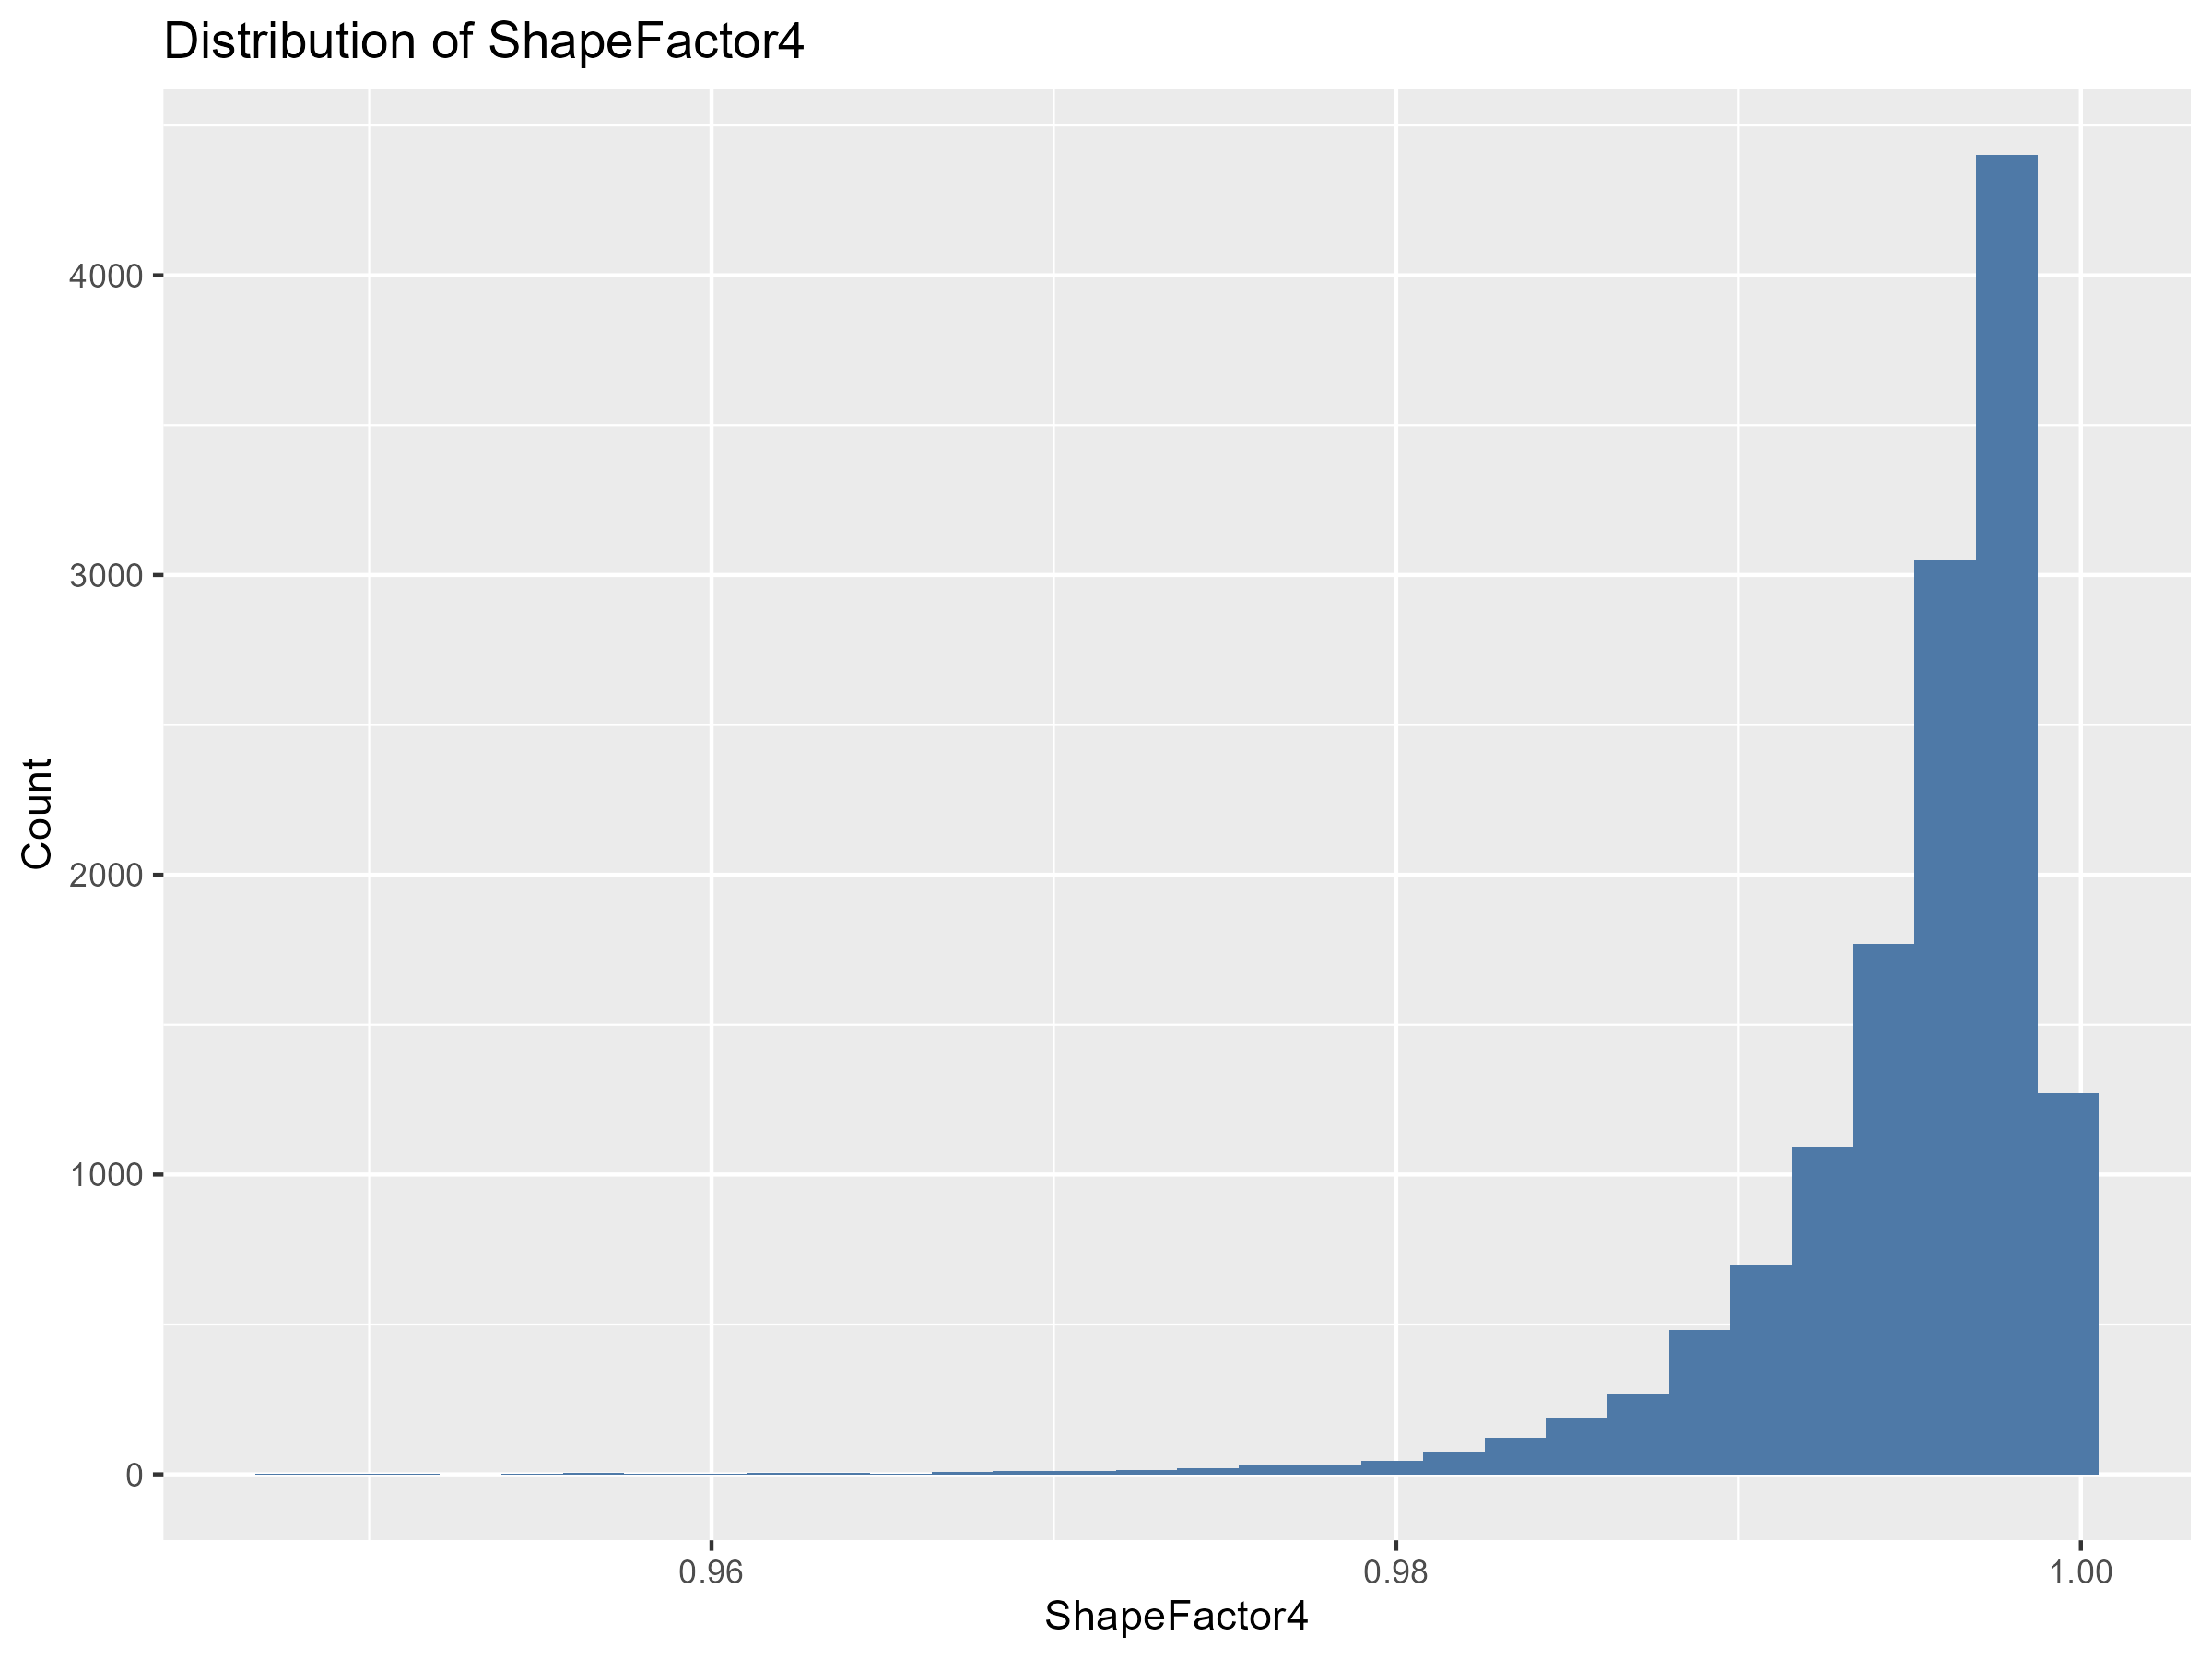
\includegraphics[width=0.8\textwidth]{graphs/histogram_shapefactor4.png}
    \caption{Histogram of ShapeFactor4}
    \label{fig:histogram_shapefactor4}
\end{figure}
This histogram illustrates the distribution of ShapeFactor4 values across the dataset. The x-axis represents the ShapeFactor4 values, while the y-axis shows the count of instances for each value range. The distribution is heavily right-skewed, with most data points concentrated near 1.0. The highest count occurs around values close to 1.0, while very few instances have ShapeFactor4 values below 0.97.

\newpage

\subsection{Bar Plot of Average Roundness by Bean Class}
\noindent\textbf{Objective:} This bar plot compares the average \textit{Roundness} for each bean class, answering: "Which bean classes exhibit higher or lower average roundness?"

\noindent\textbf{Explanation:} The bar plot shows the average roundness values for each bean class, indicating differences in shape regularity. Classes with higher average roundness values tend to have more circular shapes, while those with lower values may have more elongated or irregular shapes.

\begin{figure}[H]
    \centering
    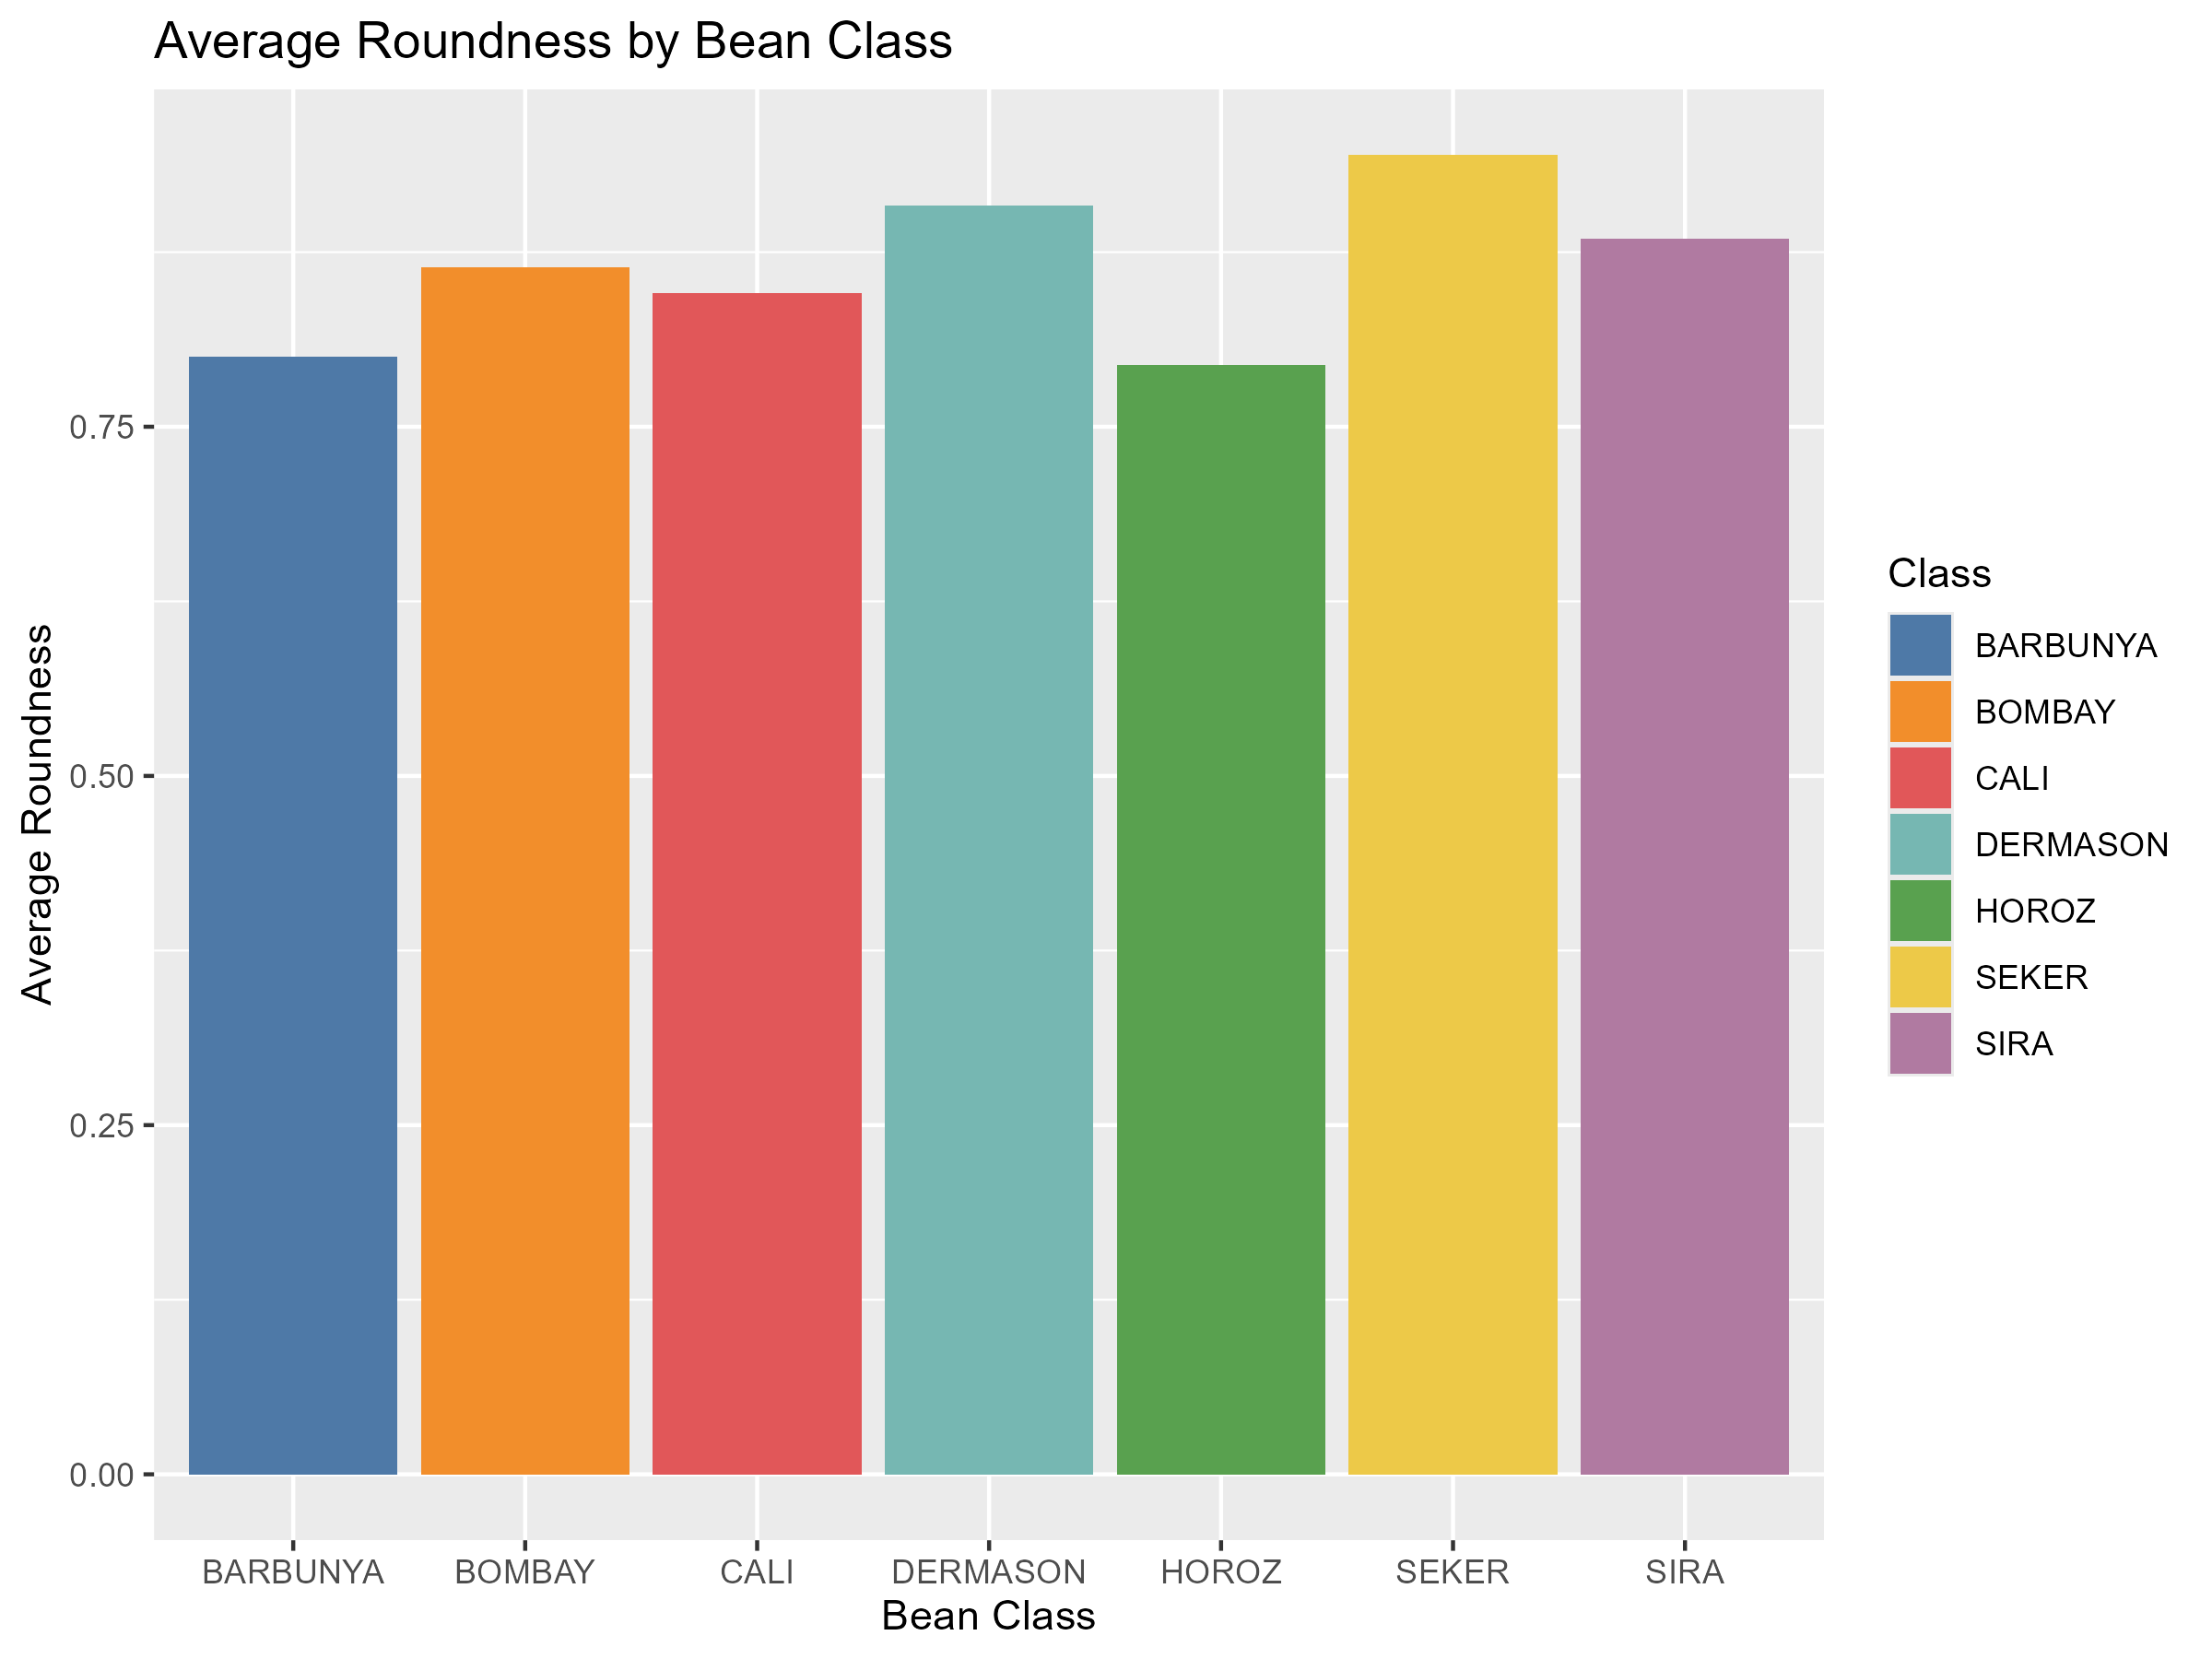
\includegraphics[width=0.8\textwidth]{graphs/barplot_roundness.png}
    \caption{Bar Plot of Average Roundness by Bean Class}
    \label{fig:barplot_roundness}
\end{figure}
This bar plot shows the average Roundness values for each bean class. The x-axis lists the different bean classes, while the y-axis represents their average roundness, ranging from 0 to 1. All classes have roundness values close to 0.75, with minor differences among them. DERMASON and SEKER have slightly higher average roundness, while HOROZ has the lowest..

\newpage

\subsection{Boxplot of Compactness by Bean Class}
\noindent\textbf{Objective:} This boxplot compares the distribution of \textit{Compactness} across different bean classes, answering: "How does compactness vary among the different bean types?"

\noindent\textbf{Explanation:} The boxplot displays the median, interquartile range, and any outliers for compactness values across bean classes. Classes with higher median compactness values are more likely to have more regular, circular shapes, while those with lower median values may have more irregular shapes. The spread and presence of outliers indicate variability within each class.

\begin{figure}[H]
    \centering
    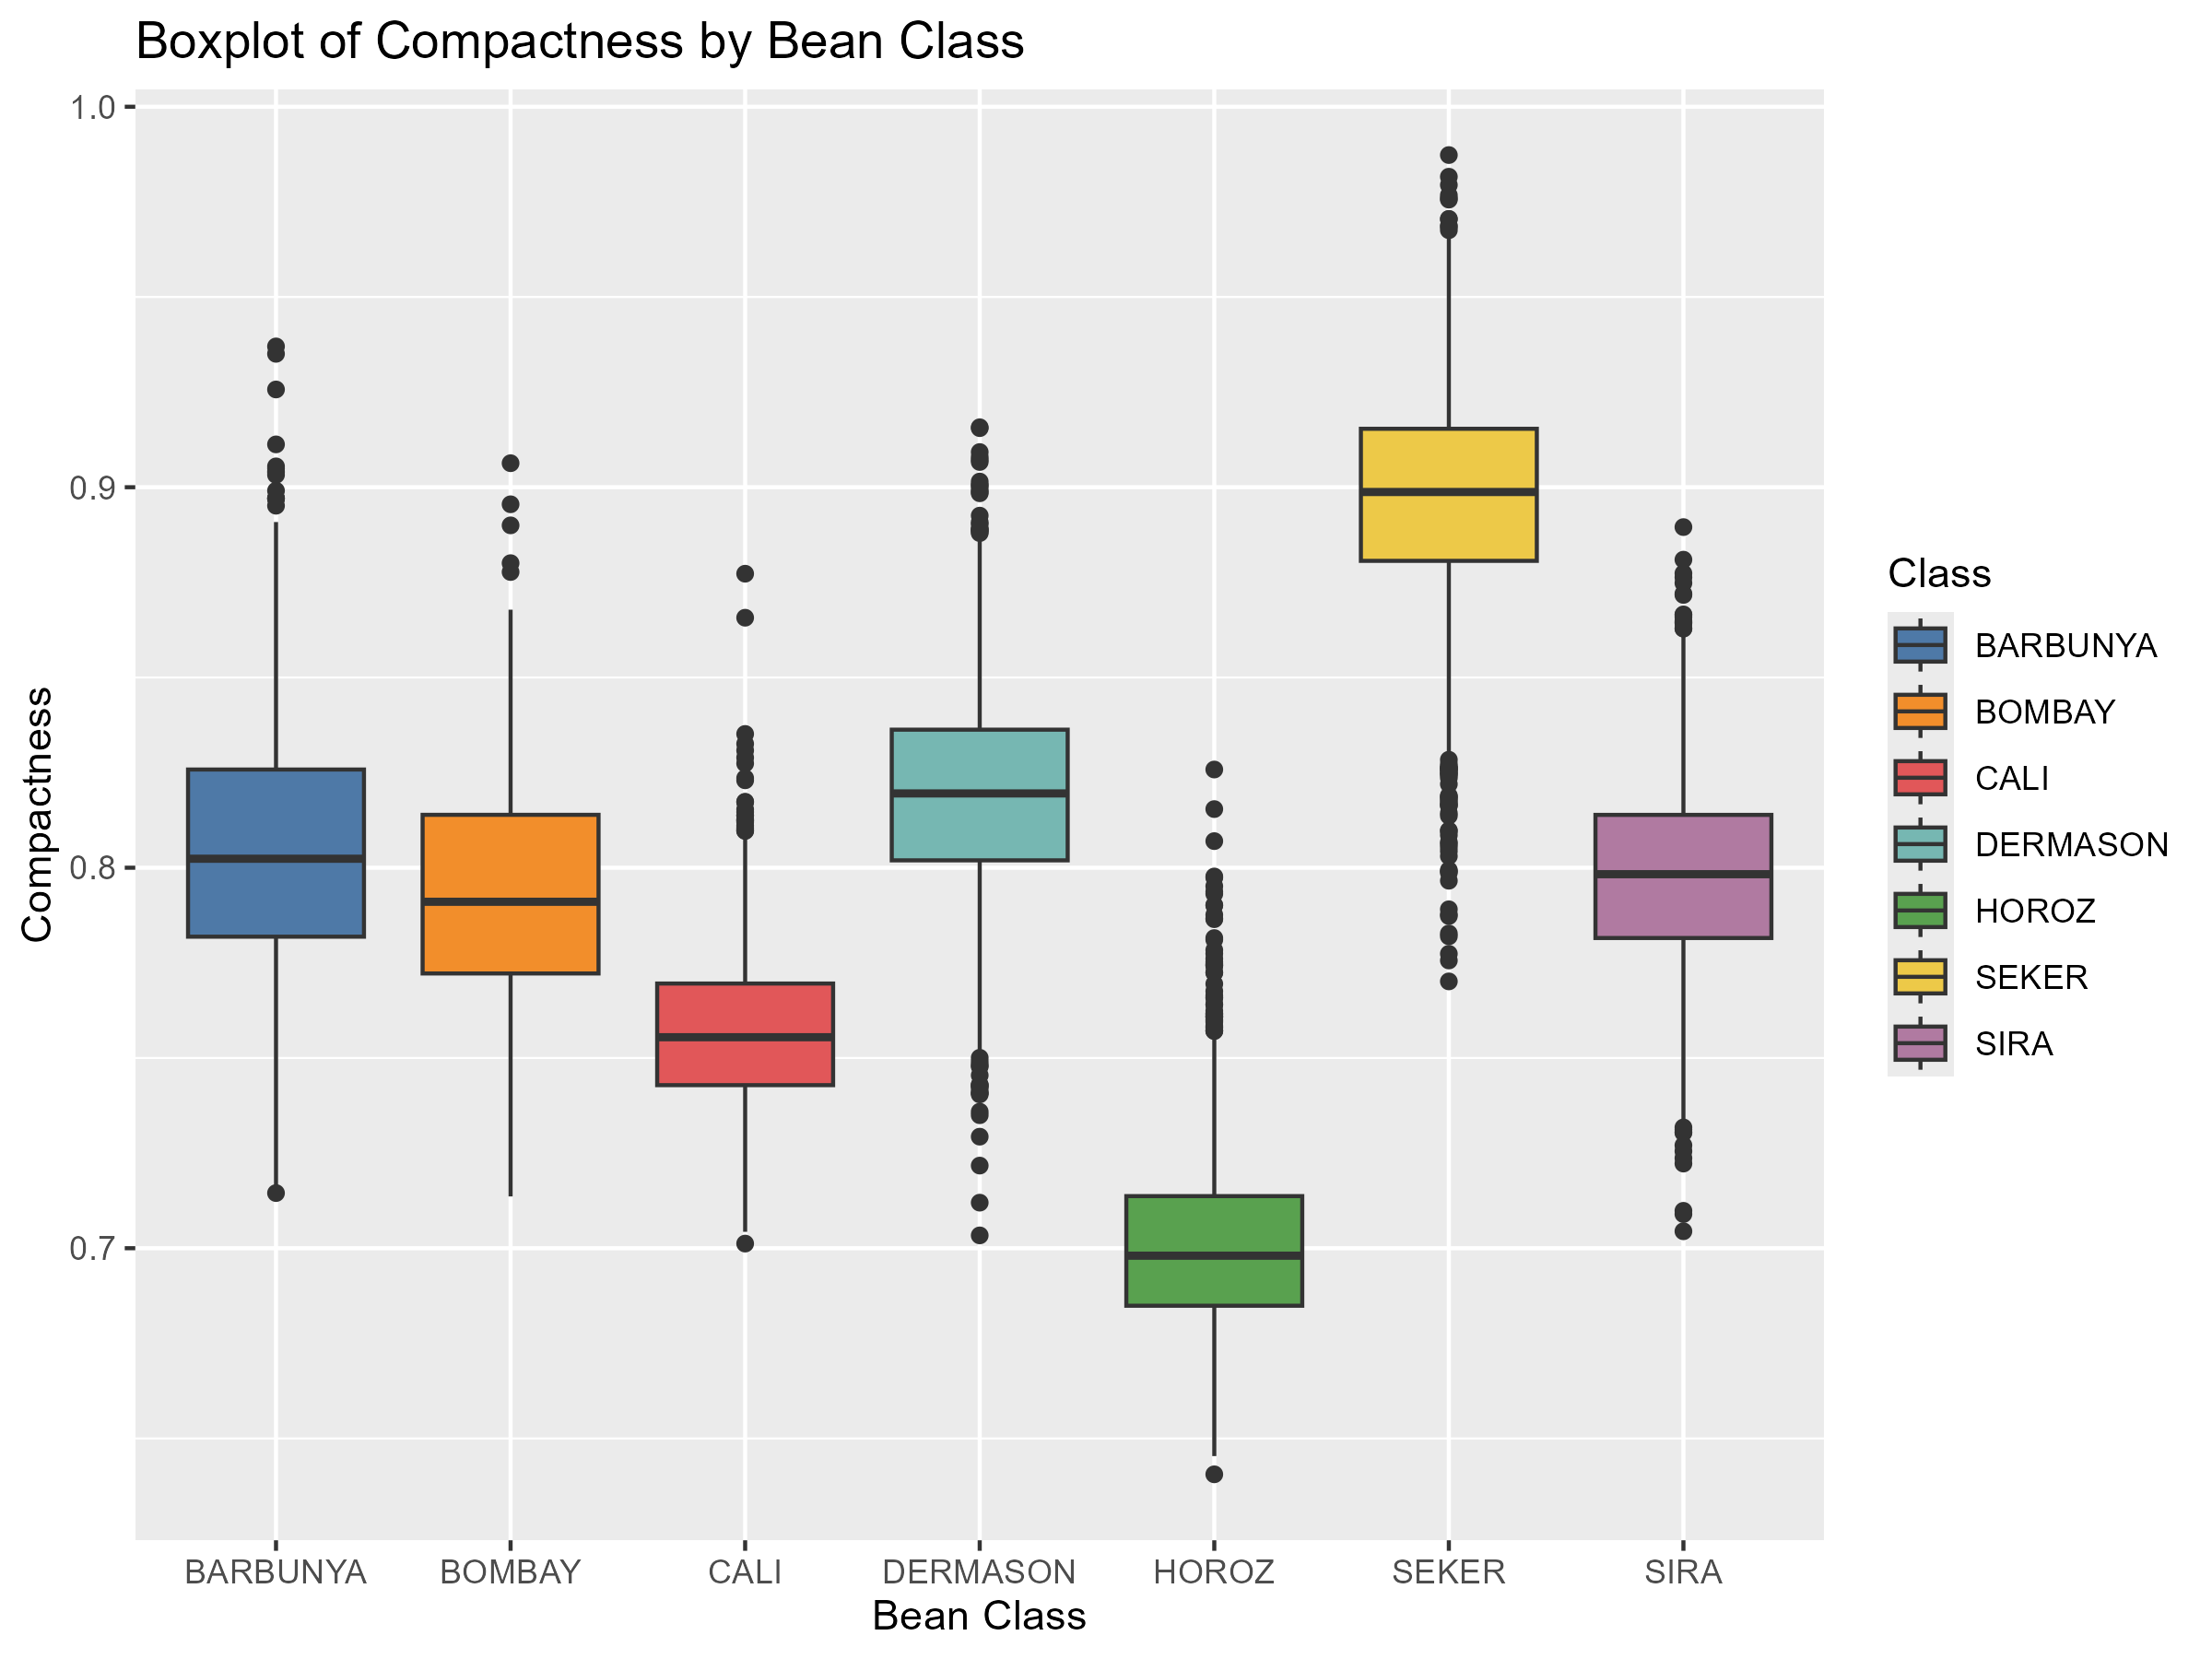
\includegraphics[width=0.8\textwidth]{graphs/boxplot_compactness.png}
    \caption{Boxplot of Compactness by Bean Class}
    \label{fig:boxplot_compactness}
\end{figure}
This boxplot displays the distribution of Compactness for different bean classes. The x-axis represents the bean classes, while the y-axis shows the compactness values. Each box shows the interquartile range (IQR), with the line inside indicating the median. DERMASON and SEKER have the highest compactness medians, while HOROZ and CALI show lower compactness values. Outliers, represented by dots, are present in classes like SEKER and HOROZ, indicating beans with unusually high or low compactness values compared to others.

\newpage

\section{Summary and Conclusion}
The analysis of the Dry Bean Dataset provided valuable insights into the physical features of different bean types. Key conclusions include:
\begin{itemize}
    \item \textbf{Feature Correlations}: Strong correlations were found between features like Area, Perimeter, and Major Axis Length, indicating their usefulness for classification.
    
    \item \textbf{Class Variability}: Variations in features such as Area and Compactness among bean classes highlight their importance in distinguishing classes and improving classification.
    
    \item \textbf{Feature Utility}: Features like Compactness and Roundness, combined with metrics like Aspect Ratio, provide a reliable profile for each bean class.
    
    \item \textbf{Implications for Agriculture}: Insights from this analysis can help automate sorting and quality control of dry beans, ensuring consistent quality and reducing manual labor \cite{sandeep2022modern}.
\end{itemize}

Overall, the analysis highlights the importance of both size and shape features in distinguishing bean types, providing a basis for using machine learning models for accurate classification with practical applications in agriculture.
\newpage

\subsection{Non-trivial Questions and Answers}
\begin{itemize}
    \item \textbf{Q1: What is the most significant correlation observed in the dataset?}\\
    \textbf{Reason:} This is a non-trivial question because understanding which features have strong correlations helps in feature selection for machine learning models. Highly correlated features may not add new information to the model, so identifying these can guide dimensionality reduction techniques.\\
    \textbf{Ans:} From the correlation heatmap (\autoref{fig:correlation_heatmap}), it is evident that 'Major Axis Length' and 'Perimeter' are highly correlated, indicating that larger beans tend to have longer perimeters.

    \item \textbf{Q2: Which feature exhibits the greatest variance across bean classes?}\\
    \textbf{Reason:} This is a non-trivial question because identifying features with high variance is crucial in classification tasks, as these features are more likely to differentiate between classes effectively. Low-variance features might contribute little to the model's ability to distinguish classes.\\
    \textbf{Ans:} The 'Area' feature shows the greatest variance across bean classes, as shown in the density plot (\autoref{fig:density_area}). This suggests that 'Area' could be a distinguishing feature for classification.

    \item \textbf{Q3: What relationship between compactness and roundness is observed?}\\
    \textbf{Reason:} This is a non-trivial question because exploring the relationship between shape features like compactness and roundness helps in understanding the geometric properties that can be used to classify different bean types, which may not be apparent from size-related features alone.\\
    \textbf{Ans:} There is a noticeable trend that as the 'Compactness' of a bean increases, its 'Roundness' also increases. This relationship is more pronounced in certain bean classes, as seen in the scatter plot (\autoref{fig:scatter_roundness_compactness}).

    \item \textbf{Q4: How do the different bean classes overlap in terms of shape factors, and what implications does this have for classification?}\\
    \textbf{Reason:} This is a non-trivial question because overlapping distributions indicate potential challenges in classifying bean types based solely on these features, requiring more complex models or combinations of features for accurate classification.\\
    \textbf{Ans:} There is noticeable overlap among bean classes in `ShapeFactor1` and `ShapeFactor3` (\autoref{fig:density_shapefactor1} and \autoref{fig:density_shapefactor3}). This suggests that some classes share similar geometric properties, making classification challenging. Combining multiple features and using advanced techniques like dimensionality reduction could help improve class separation and model accuracy.

    \item \textbf{Q5: What effect does the variability in aspect ratio have on distinguishing bean types?}\\
    \textbf{Reason:} This is a non-trivial question because aspect ratio provides information on elongation, which can differentiate classes. However, its effectiveness is limited when distributions overlap, requiring a multi-feature approach to improve classification.\\
    \textbf{Ans:} The variability in aspect ratio, as seen in the violin plot (\autoref{fig:violin_aspect_ratio}), indicates it can help distinguish elongated beans like HOROZ from more compact ones. However, due to overlap between classes, aspect ratio alone isn't sufficient and should be combined with features like compactness for better classification.

    \item \textbf{Q6: Which features show the least correlation, and how might these features contribute to the classification?}\\
    \textbf{Reason:} This is a non-trivial question because features with low correlation may still add valuable information for classification because they provide independent characteristics not captured by other features. Understanding this can improve model performance by including diverse feature types.\\
    \textbf{Ans:} Features like \textit{Solidity} and \textit{ShapeFactor2} show weaker correlations (\autoref{fig:correlation_heatmap}), but they capture unique shape details that more correlated features miss. Including them can enhance model robustness by adding diverse information for classification.

    \item \textbf{Q7: How does the distribution of convex area compare across bean types?}\\
    \textbf{Reason:} This is a non-trivial question because evaluating the distribution of features like convex area can reveal important class-specific characteristics that may not be obvious in other plots, assisting in feature selection for classification models.\\
    \textbf{Ans:} The histogram of convex area (\autoref{fig:histogram_convex_area}) shows a right-skewed distribution, with most beans having lower convex area values. BOMBAY beans tend to have larger convex areas, which may help differentiate them from other types.

    \item \textbf{Q8: What insights can be drawn from the scatter plot of convex area vs area?}\\
    \textbf{Reason:} This is a non-trivial question because understanding the correlation between area-related features helps in feature engineering and selection, potentially revealing redundant or complementary features for classification models.\\
    \textbf{Ans:} The scatter plot (\autoref{fig:scatter_convex_area}) shows a strong positive correlation between convex area and area, indicating that larger beans also have larger convex areas. BOMBAY beans tend to have higher values for both, suggesting they are consistently larger in size.

    \item \textbf{Q9: How do beans' eccentricity values relate to their classification?}\\
    \textbf{Reason:} This is a non-trivial question because eccentricity provides insight into the shape and orientation of beans, which are key factors in classification. Recognizing which classes tend to have higher or lower eccentricity can improve model accuracy.\\
    \textbf{Ans:} Beans like HOROZ and SIRA have higher median eccentricity values, indicating they are more elongated compared to other classes (\autoref{fig:boxplot_eccentricity}). This characteristic can be used to distinguish elongated beans from more rounded ones.

\end{itemize}




\newpage

\section{Future Enhancements}
The current analysis lays the foundation for future research on classification models for the Dry Bean Dataset. Future enhancements could include:
\begin{itemize}
    \item \textbf{Feature Engineering}: Deriving new metrics from existing features to enhance classification accuracy and employing feature selection to improve model efficiency.
    
    \item \textbf{Advanced Visualization Techniques}: Using 3D plots and dimensionality reduction techniques like t-SNE or PCA to better represent high-dimensional data and reveal patterns among bean classes.

    \item \textbf{Machine Learning Models}: Implementing advanced classification algorithms such as SVM, Random Forests, Gradient Boosting, or deep learning to improve accuracy \cite{khan2023comparison}. Techniques like hyperparameter tuning and model ensembling can further enhance model performance.

    \item \textbf{Interactive Dashboards}: Developing an advanced Shiny dashboard with real-time data analysis, user-friendly controls, and model predictions to provide an interactive exploration of the dataset.

    \item \textbf{Deployment and Integration}: Deploying the classification model through an API and building a user-friendly interface for practical applications in agriculture, automating quality control processes.
\end{itemize}

These enhancements aim to utilize sophisticated techniques and interactivity to improve classification accuracy and the practical usability of the developed models.

\newpage
\bibliographystyle{agsm}
\bibliography{cite}

\end{document}
